\chapter{Theory of External Optical Feedback in a Polymer-based DBR Laser}\label{ch:Theory}
In this chapter, the modelling of external feedback in the hybrid polymer-based DBR laser considered in this work, is presented. This model is set as a starting point to discuss the effects of optical feedback with regards to linewidth, modulation bandwidth and chirp.

\section{Model of External Optical Feedback in a Polymer-based DBR Laser}\label{sec:model_laser}
The effect of the external feedback in semiconductor lasers is defined by parameters of feedback coefficent $C$, coupling coefficient $\kappa_{ext}$ and chirp reduction factor $F$ \cite{kazarinov1987relation, petermann2012laser}. They are extracted by a three-mirror laser model and its equivalent two-mirror Fabry-Perot cavity as shown in \autoref{fig:laser_cavity_model} in order to correctly consider the feedback effect in the polymer-based tunable DBR laser.

\begin{figure}[ht]
    \centering
    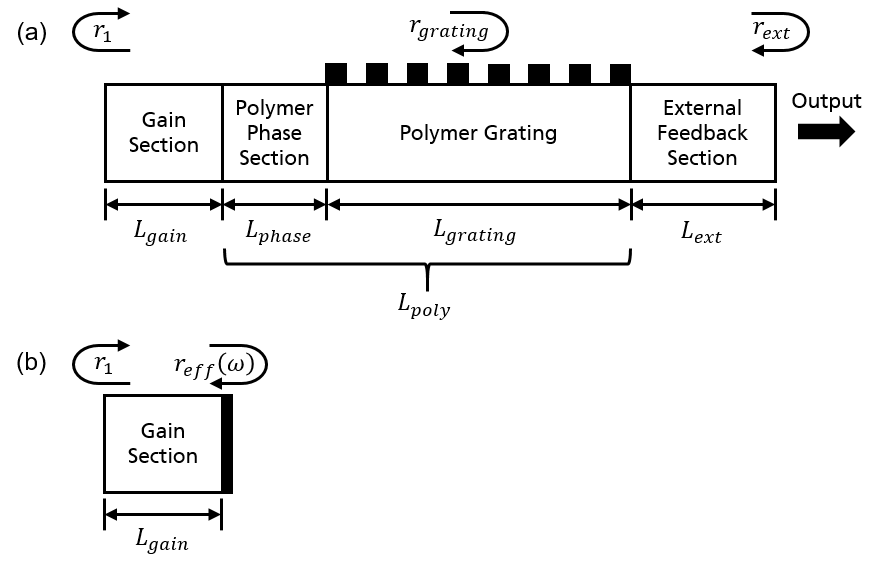
\includegraphics[width=.9\linewidth]{figures/laser_cavity_model.png}
    \caption{(a) Polymer-based tunable DBR laser with external feeback section and (b) its equivalent cavity with effective mirror to model the feedback effect.}
    \label{fig:laser_cavity_model}
\end{figure}

The InP gain section in \autoref{fig:laser_cavity_model} possesses a length of $L_{gain}$ and comprises a High Reflection (HR) coating with reflectance $r_1$ at one of its facets and an Anti-Reflection (AR) coating against polymer at the other facet. The polymer part consists a phase and a grating section with a total length of $L_{poly}$ and the external feedback section with a length of $L_{ext}$ after the grating. $r_1$, $r_{grating}$ and $r_{ext}$ are amplitude reflectance of the gain section front facet, grating and external reflector respectively.

There are two ways to describe the feedback effect by the chirp reduction factor $F$, first one is mainly concerning the feedback coefficent $C$ parameter, which characterizes the level of feedback in relation to how it affects the mode behavior of the laser and is defined as \cite{petermann2012laser}
\begin{equation}
    C=\frac{\tau_{ext}}{\tau_{gain}+\tau_{poly}}\kappa_{ext}\sqrt{1+\alpha^2}
    \label{eq:C}
\end{equation}
with
\begin{equation}
    \kappa_{ext}=\frac{r_{ext}}{r_{grating}}\qty(1-\abs{r_{grating}}^2)
    \label{eq:kappa_ext}
\end{equation}
where $\tau=2nL/c$ is the roud-trip time in the corresponding section, $\kappa_{ext}$ is the coupling coefficient from the grating reflector to the external cavity, and $\alpha$ is the linewidth enhancement factor \cite{henry1982theory}. Note that here the grating reflectivity $r_{grating}$ is considered as a constant value as shown in \autoref{fig:L_grating_eff}, which leads to effective grating length $L_{eff}=tanh(\kappa L_{grating})/2\kappa$ shorter than the real grating length $L_{grating}$ \cite{kuznetsov1988theory}. The $L_{eff}$ is then contained in the laser cavity and the rest of the grating is included in the external feedback section.

\begin{figure}[ht]
    \centering
    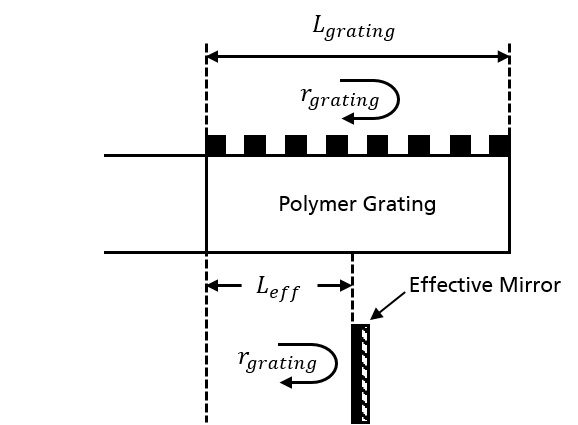
\includegraphics[width=.6\linewidth]{figures/L_grating_eff.png}
    \caption{Definition of an effective mirror for a grating reflector \cite{coldren2012diode}.}
    \label{fig:L_grating_eff}
\end{figure}

The $C$ parameter indicates that the laser stability under feedback is affected both by external reflector $r_{ext}$ and external round-trip time $\tau_{ext}$. When $C<1$, which implies weak feedback \cite{petermann2012laser,ohtsubo2012semiconductor}, the laser operates in a single mode lasing region and is phase dependent to the external feedback \cite{petermann2012laser, ohtsubo2012semiconductor}. When $C>1$, which implies medium to strong feedback \cite{petermann2012laser,ohtsubo2012semiconductor}, over one stable mode will appear and the laser will undergo a route-to-chaos behavior until it reaches coherence-collapse \cite{lenstra1985coherence} region. After the coherence-collapse region, if the feedback strength is even higher and the laser will operates in stable single mode again lasing with the compound cavity mode \cite{donati2013diagram}.

For the weak feedback region when $C<1$, chirp reduction factor $F$ is defined as \cite{petermann2012laser,coldren2012diode}
\begin{equation}
    F=1+C\cos(\phi_{ext}+\arctan\alpha)
    \label{eq:F_weak_feedback}
\end{equation}
where $\phi_{ext}=2\beta_{poly}L_{ext}$ is the round-trip phase of the external cavity.

For the case of strong feedback, which is more interesting and stable for the practical implementation, the factor $F$ becomes \cite{ishii2017narrow}
\begin{equation}
    F=1+R_{ext}\frac{\tau_{ext}}{\tau_{gain}+\tau_{poly}}.
    \label{eq:F_strong_feedback}
\end{equation}
where $R_{ext}=r_{ext}^2$ is the power reflectivity of the external reflector.
% with
% \begin{equation}
%     f_{ext}=\eta_{couple}R_{ext}
%     \label{eq:F_f_ext}
% \end{equation}
% where $\eta_{couple}$ is the coupling coefficient between the normal cavity and external cavity. This parameter is included because for the design presented in \autoref{sec:design_and_characterization}, the feedback from the external cavity is not totally coupled back to the laser cavity. However, in the case discussed above $\eta_{couple}=1$.
% Rate equation models of the field and phase including the time delay of the feedback field reveal unstable solutions and chaotic behavior at these high feedback levels \cite{tkach1986regimes}. The collapse begins at the transition to regime IV, where the normally small satellite peaks created by noise-induced relaxation oscillations (depicted in Fig. 5.23) grow larger and larger, eventually becoming comparable to the central peak and broadening the linewidth dramatically \cite{coldren2012diode}.
% \subsection{Chirp Reduction Factor $F$ for weak feedback condition}
% There are two ways to define the chirp reduction factor $F$, 

% \subsection{Chirp Reduction Factor $F$ for weak feedback condition}
% The other is suitable for all the conditions, both will be discussed here.

Seconde way to define the chirp reduction factor $F$ is not only relate to round-trip time in each section but also to the frequency dependence of the reflection coefficient of the reflector \cite{petermann2012laser}. In this work it is done by considering the equivalent two-mirror cavity and replacing the external feedback part with an effective mirror reflectivity $r_{eff}(\omega)$ as shown in \autoref{fig:laser_cavity_model} (b), $r_{eff}(\omega)$ is modifed according to \cite{kazarinov1987relation, coldren2012diode, komljenovic2015widely}
\begin{equation}
    r_{eff}(\omega)=r(\omega)exp\qty(-i\varphi_{eff}(\omega))=\frac{r_{grating}(\omega)+r_{ext}W_1}{1+r_{grating}(\omega)r_{ext}W_1}W_2
    \label{eq:effective_reflectivity}
\end{equation}
\begin{equation}
    W_1=e^{-\alpha_{poly}L_{ext}}e^{-2i\beta_{poly}L_{ext}}
    \label{eq:propogation_external_cavity}
\end{equation}
\begin{equation}
    W_2=e^{-\alpha_{poly}L_{phase}}e^{-2i\beta_{poly}L_{phase}}
    \label{eq:propogation_polymer_wg}
\end{equation}
where $\alpha_{poly}$ is the polymer waveguide propagation modal loss and $\beta_{poly}=2\pi n_{poly}/\lambda$ is the effective propagation constant for the lasing mode, $r_{grating}(\omega)$ is the frequency-dependent complex amplitude reflectance of the grating reflector \cite{yariv1977periodic}.
The chirp reduction factor $F$ is then defined as \cite{kazarinov1987relation, petermann2012laser}
\begin{equation}
    F=1+A+B
    \label{eq:F_factor}
\end{equation}
with
\begin{equation}
    A=\frac{1}{\tau_{gain}}\qty(\dv{\omega}\varphi_{eff}(\omega))
    \label{eq:F_factor_A}
\end{equation}
\begin{equation}
    B=\frac{\alpha}{\tau_{gain}}\qty(\dv{\omega}\ln{r_{eff}(\omega)})
    \label{eq:F_factor_B}
\end{equation}
where $\alpha$ is the linewidth enhancement factor \cite{henry1982theory}, the parameter $A$ is related to the freqeuncy derivative of the phase $\varphi_{eff}(\omega)$ in \autoref{eq:effective_reflectivity}, which denotes the ratio of the external cavity path length to the gain section path length. It can be interperated as the ratio of the photon numbers outside to inside the gain medium, which remains nearly constant once the laser cavity is formed \cite{choi2015evaluation}. By designing a cavity with a long external cavity, a large $A$ can be achieved. On the other hand, the parameter $B$ accounts for the wavelength dependence of the spectral reflectivity. It is changed if the lasing mode is detuned away from the Bragg wavelength under detuned loading conditions \cite{feiste1998optimization, kjebon1997two, chacinski2010impact} which will be discussed further in \autoref{sec:bandwidth_enhancement}. Additional reduction occurs only at the rising slope of the grating response which generates a positive $B$ value.


\section{Chirp Reduction}\label{sec:chirp_reduction}
Light chirping can be defined as the instantaneous change of the central wavelength or optical frequency in response to variations in the optical power \cite{villafranca2007precise}. Two main contributions of the frequency chirp are distinguished, one is an adiabatic chirp, producing a frequency shift proportional to the instantaneous optical power, and is defined by parameter $\alpha_{adiabatic}$, which is associated to the nonlinear gain \cite{villafranca2007precise, harder1983measurement}. Another one is a transient chirp component that evolve with the time deriative of the optical power, and is defined by $\alpha_{transient}$, normally named as linewidth enhancement factor \cite{henry1982theory} and dominates when dealing with semiconductor lasers \cite{choi2015evaluation}. 
% Here only the transient chirp $\alpha$ is considered and is defined as \cite{henry1982theory, soriano2013complex}
% \begin{equation}
%     \alpha=-\frac{\dv*{\chi_r(n)}{n}}{\dv*{\chi_i(n)}{n}}
% \end{equation}
% with $\chi_r$ and $\chi_i$ are the real and imaginary parts of the carrier-dependent susceptibility of the semiconductor material.

% Since the linewidth enhancement factor $\alpha$ is highly phase dependent, two measurement methods are performed to get the right characterization for DBR laser with feedback.

% i.e. a residual frequency modulation of an amplitude modulated optical wave
% the $\alpha$ parameter is defined as 

The chirp reduction for laser coupled with a passive cavity is related to $F$ and is defined as \cite{choi2015evaluation,kazarinov1987relation, petermann2012laser}
\begin{equation}
    \alpha_{adiabatic}\approx\frac{\alpha}{1+A+B}
    \label{eq:chirp_reduction_adiabatic}
\end{equation}
\begin{equation}
    \alpha_{transient}\approx\frac{\alpha(1+A-B/\alpha^2)}{1+A+B}.
    \label{eq:chirp_reduction_transient}
\end{equation}
Note that adiabatic chirp is usually frequency-independent and dominant at low modulation frequency, but for the semiconductor laser operating at large modulation frequency over $10 \ Gb/s$, it is sufficient to consider only the transient chirp \cite{choi2015evaluation}, which will be the one discussed in this thesis. 

\section{Linewidth Reduction}\label{sec:linewidth_reduction}
Linewidth reduction for laser coupled with a passive cavity is related to $F$ and is defined as \cite{kazarinov1987relation, petermann2012laser}
\begin{equation}
    \Delta\nu=\frac{\Delta\nu_0}{F^2}
    \label{eq:linewidth_reduction}
\end{equation}
where $\Delta\nu$ and $\Delta\nu_0$ are the linewidth with and without feedback respectively. 

For the weak feedback case, \autoref{eq:F_weak_feedback} shows that the linewidth can either be narrowed $\Delta\nu_0/(1+C)^2$ or broadened $\Delta\nu_0/(1-C)^2$ depending on the feedback phase. Apart from that, \autoref{eq:F_factor} shows further linewidth reduction can be achieved by considering the wavelength dependence of the spectral reflectivity introduced with parameter $B$.
% If $\Delta\omega_0$ is denoted as the adiabatic chirp in the absence of feedback, then the chirp with external cavity $\Delta\omega$ is obtained as \cite{kazarinov1987relation}
% \begin{equation}
%     \Delta\omega=\frac{\Delta\omega_0}{F}
%     \label{eq:chirp_reduction}
% \end{equation}
% if the spectral linewidth without external feedback is denoted by $\Delta\nu_0$, the spectral linewidth with the external cavity $\Delta\nu$ is simply obtianed as \cite{}
% \begin{equation}
%     \Delta\nu=\frac{\Delta\nu_0}{F^2}
%     \label{eq:linewidth_reduction}
% \end{equation}

With \autoref{eq:F_weak_feedback} and \autoref{eq:F_strong_feedback} the linewidth reduction factor $F^2$ versus the external cavity length can be calculated and is shown in \autoref{fig:F_reduction_factor}. Vertical dashed line $L_c$ indicates more modes may starts to appear where the $C$ parameter reaches 1 \cite{petermann2012laser}. \autoref{fig:F_reduction_factor} is caculated under the assumption that the feedback comes from the output waveguide facet, which is formed by a polymer/air interface and leads to $R_{ext}=0.035$. The parameters used for calculation is shown in \autoref{tab:F_reduction_factor}.

\begin{table}[ht]
    \centering
    \caption{Parameters used for the calculation of the linewidth reduction factor $F^2$.}
    \begin{tabular}{@{}lll@{}}
    \toprule
    Symbol        & Description                  & Value           \\ \midrule
    $L_{gain}$    & Active section length        & 300 $\mu m$     \\
    $L_{phase}$   & Phase section length         & 525 $\mu m$     \\
    $L_{grating}$ & Grating section length       & 699.84 $\mu m$  \\
    $n_{gain}$    & Active section refractive index  & 3.2         \\
    $n_{poly}$    & Polymer refractive index     & 1.46            \\
    $\alpha$      & Linewidth redcution factor   & -3              \\
    $R_{grating}$ & Grating reflectivity         & 0.3             \\
    $R_{ext}$     & External cavity reflectivity & 0.035           \\ \bottomrule
    \end{tabular}
    \label{tab:F_reduction_factor}
\end{table}

\begin{figure}[ht]
    \centering
    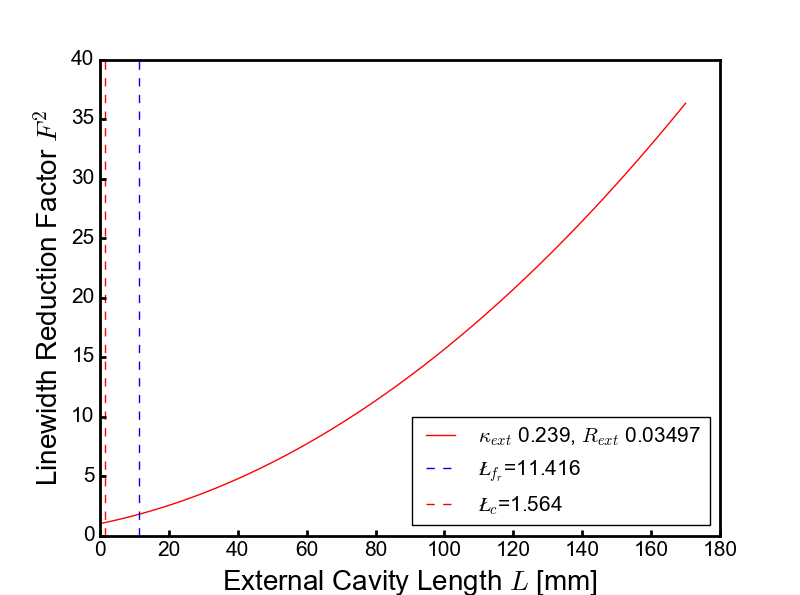
\includegraphics[width=.7\linewidth]{figures/F_reduction_factor.png}
    \caption{Calculated linewidth reduction factor $F^2$ assuming the feedback comes from the polymer/air interface. Dashed vertical line $L_c$ indicates the length where the $C$ parameter reaches 1 and more modes start to appear.}
    \label{fig:F_reduction_factor}
\end{figure}

\section{Bandwidth Enhancement}\label{sec:bandwidth_enhancement}
The maximum bit rate achieved by direct modulated lasers is typically limited by the well known resonance between carriers and photons, which is usually named as the carrier-photon resonance or the relaxation oscillation \cite{coldren2012diode}. Three approaches to achieve broader bandwidth are explored in detail here. 

\subsection{Detuned Loading Condition}\label{subsec:detuned_loading}
The first mechanism used to extend the modulation bandwidth of a semiconductor laser is the detuned loading effect, which is due to the frequency dependence of the reflection coefficient introduced by a distributed mirror (e.g. DBR \cite{feiste1998optimization, kjebon1997two, chacinski2010impact}). It can be achieved without any external feedback. 

The operation principle of the detuned loading condition can be illustrated by the calculated round-trip gain $G$ curve, which is based on the effective laser cavity model presented in \autoref{sec:model_laser} and is definied as \cite{petermann2012laser, vallone2011enhanced}
\begin{equation}
    G=r_1e^{-2i\tilde{\beta}_{gain}L_{gain}}r_{eff}(\omega)=\abs{G}e^{i\varphi(\omega)}
    \label{eq:RTG_RTP}
\end{equation}
with \cite{coldren2012diode}
\begin{equation}
    \tilde{\beta}_{gain}=\beta+i\beta_{i}=\beta+\frac{i}{2}(g-\alpha_{in})
    \label{eq:beta_gain}
\end{equation}
where the real part $\beta=2\pi n_{gain}/\lambda$ is the propagration constant inside the gain medium, and the imaginary part consists of the modal gain $g$ and the internal modal loss $\alpha_{in}$ in the gain medium \cite{coldren2012diode}. Cavity modes are obtianed when roud-trip gain in \autoref{eq:RTG_RTP} equals to 1 and the phase fulfulls the integer values of $\varphi/2\pi$, e.g. for the lasing mode $m$ at threshold one get \cite{vallone2011enhanced}
\begin{equation}
    \abs{G(\lambda_m)}=G_m=1,\ \varphi_m=2m\pi
    \label{eq:lasing_condition}
\end{equation}
these two conditions allow to numerically find the lasing mode wavelength $\lambda_m$.

Parameters given in \autoref{tab:detuned_loading} were used to calculate the round-trip gain in a DBR laser cavity without feedback and the result is shown in \autoref{fig:detuned_loading_principle}.

\begin{table}[ht]
    \centering
    \caption{Parameters used for the calculation for the round-trip gain curve in a three-section DBR laser cavity.}
    \label{tab:detuned_loading}
    \begin{tabular}{@{}lll@{}}
    \toprule
    Symbol        & Description                         & Value            \\ \midrule
    $L_{gain}$    & Active section length               & $300 \ \mu m$    \\
    $L_{phase}$   & Phase section length                & $525 \ \mu m$    \\
    $L_{grating}$ & Grating section length              & $700.644\ \mu m$ \\
    $\kappa$      & Grating coupling coefficient        & 9.80 $cm^{-1}$   \\
    $n_{gain}$      & Active section refractive index  & 3.2               \\
    $n_{poly}$    & Polymer refractive index            & 1.46             \\
    $r_1$         & Gain section  reflectivity          & 0.99             \\ \bottomrule
    \end{tabular}
\end{table}

\begin{figure}[H]
    \centering
    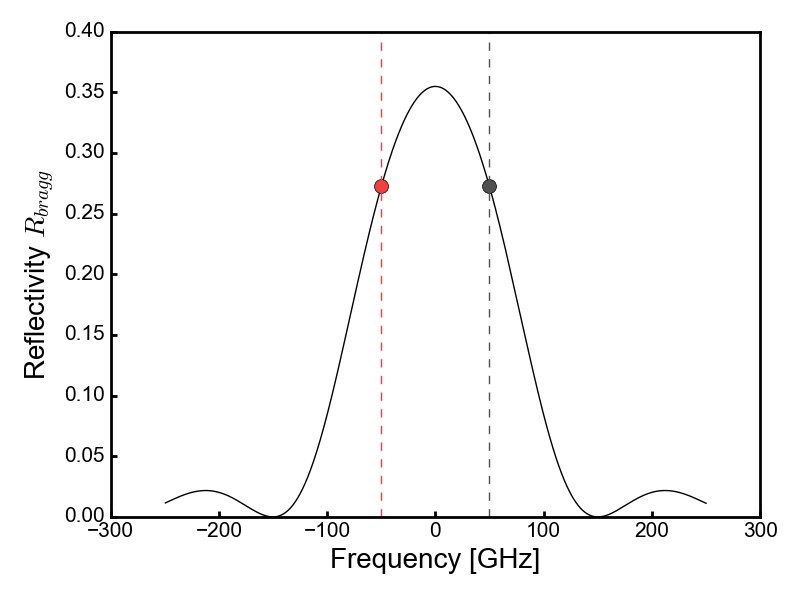
\includegraphics[width=.7\linewidth]{figures/detuned_loading_principle.png}
    \caption{Detuned loading condition with respect to the round-trip gain. The red and grey markers correspond to the lasing mode detuend to the longer and shorter wavelength sides.}
    \label{fig:detuned_loading_principle}
\end{figure}

Detuned loading condition can be achieved by positioning the lasing mode at a slightly higher wavelength respect to the Bragg wavelength, as the red marker in \autoref{fig:detuned_loading_principle}. It is reported that when the laser is operating at the longer wavelength side, an enhancement of modulation speed, reduction of phase noise (linewidth), and suppression of FM modulation (chirping) can be achieved \cite{vahala1984detuned}. 

The enhancement of the relaxation oscillation by detuned loading condition follows the same parameters $A$ and $B$ as defined in \autoref{eq:F_factor_A} and \autoref{eq:F_factor_B}, which is given by \cite{agrawal1988modulation}
\begin{equation}
    \frac{f_r^2}{f_{0}^2}=\frac{1+A+B}{(1+A)^2+(B/\alpha)^2}
    \label{eq:RO_frequency}
\end{equation}
\begin{equation}
    \frac{\gamma_r}{\gamma_{0}^2}=\frac{1+A}{(1+A)^2+(B/\alpha)^2}
    \label{eq:RO_damping}
\end{equation}
where $f_r$ and $\gamma_r$ are the frequency and the damping rate of the relaxation oscillation, $f_{0}$ and $\gamma_0$ are the value for the solitary laser. As the parameter $B$ indicates the slope of the grating response, by tuning towards the longer wavelength side, a positive $B$ value can be achieved, thus an increase in the relaxation oscillation and lower damping value can be achieved according to \autoref{eq:RO_frequency} and \autoref{eq:RO_damping}.

% The detuned loading of the laser cavity increases the interaction between the photons and the free carriers in the laser cavity which will both increase the modulation bandwidth and reduce the variation of the carrier density during modulation \cite{kjebon2002experimental}. This is because, in the longer wavelength region, the increase in carrier density increases the material gain while reducing the mirror loss (i.e. increase the reflection from the grating). As a result, the effective differential gain is increased, which, in turn, reduces the effective linewidth enhancement factor \cite{vahala1984detuned, chacinski2010impact}.




% \begin{figure}[!htb]
%   \begin{minipage}{0.48\textwidth}
%      \centering
%      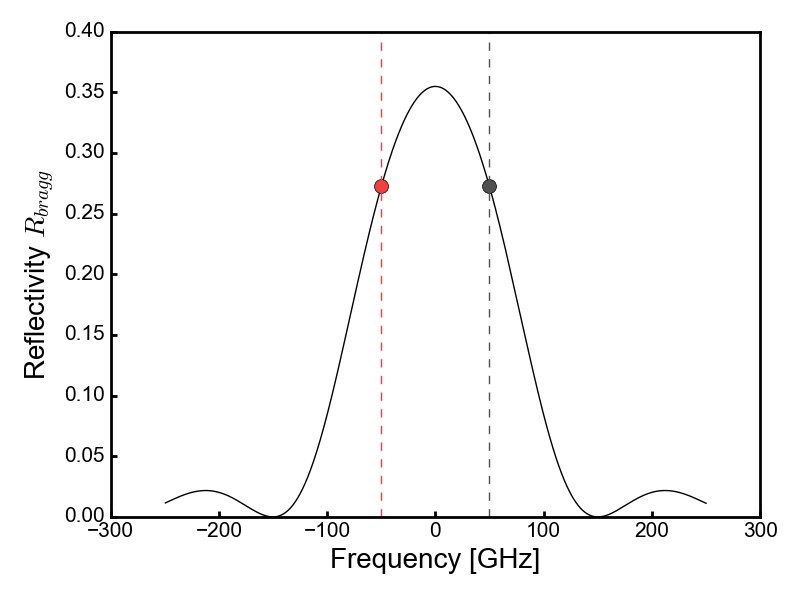
\includegraphics[width=.7\linewidth]{figures/detuned_loading_principle.png}
%      \caption{Detuned loading operation principle}
%      \label{fig:detuned_loading_principle}
%   \end{minipage}\hfill
%   \begin{minipage}{0.48\textwidth}
%      \centering
%      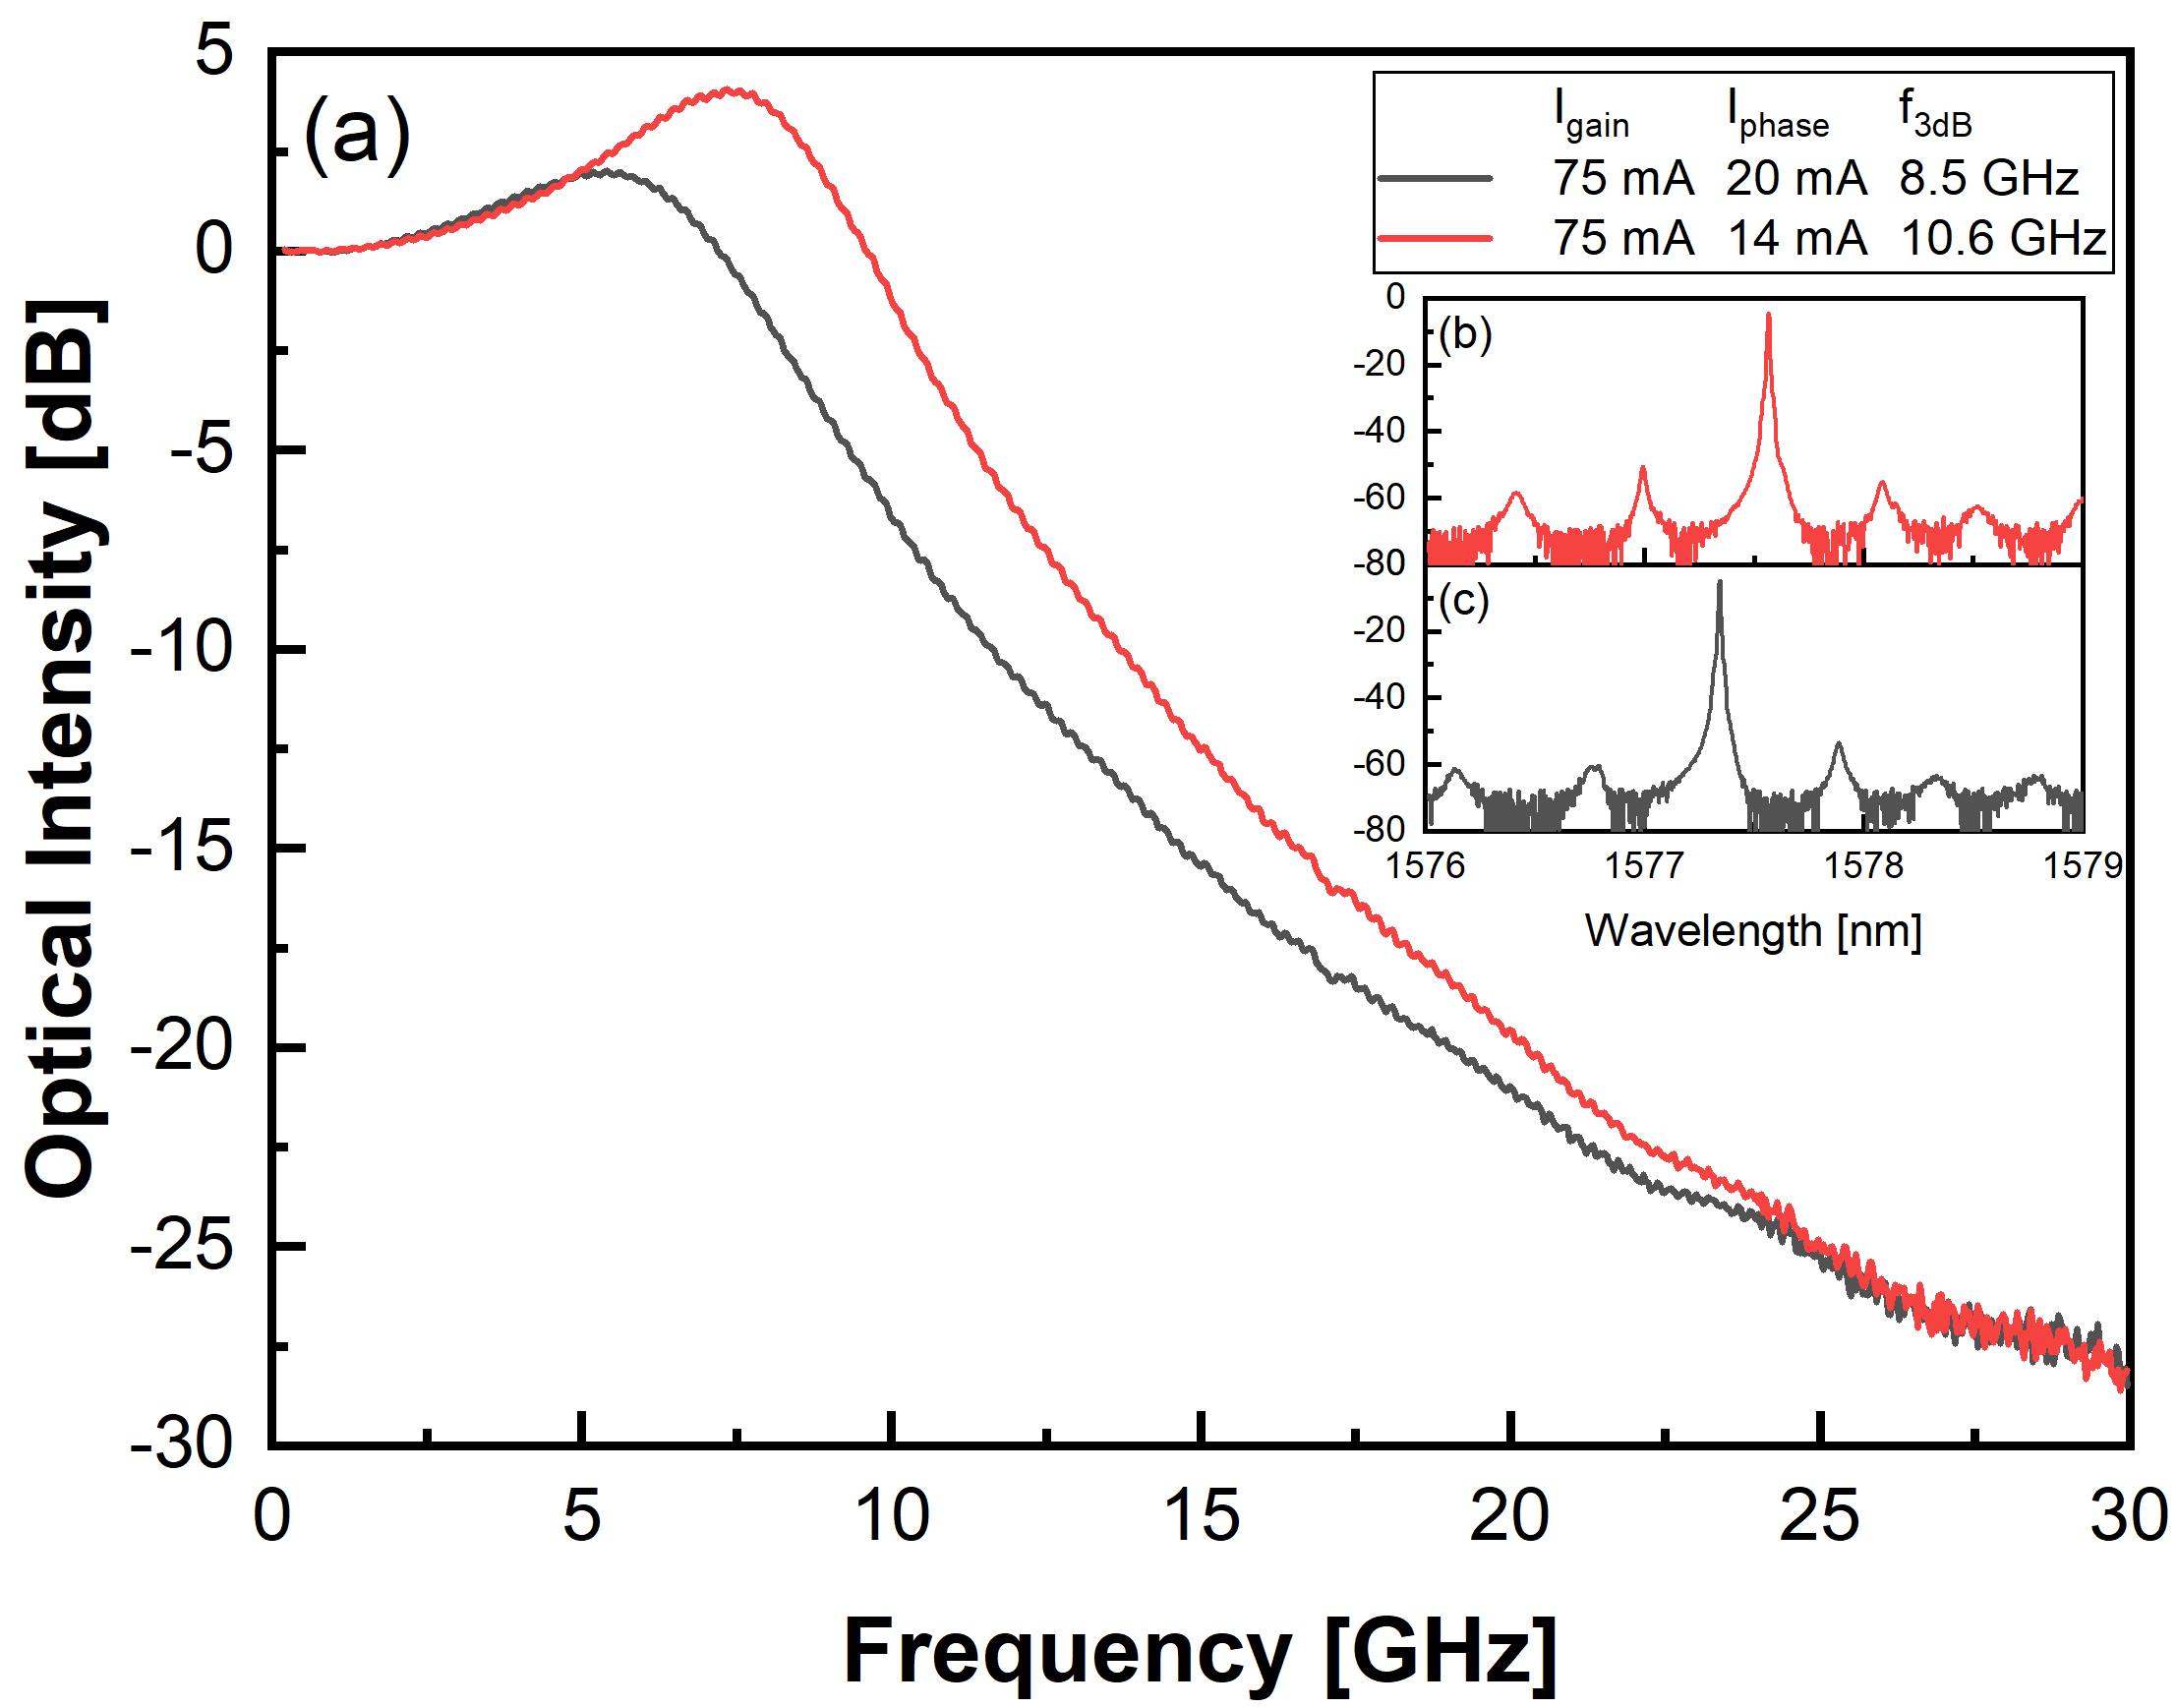
\includegraphics[width=.7\linewidth]{figures/detuned_loading.png}
%      \caption{Laser under detuned loading condition}
%      \label{fig:detuned_loading}
%   \end{minipage}
% \end{figure}

\subsection{Feedback Introduced Detuned Loading}\label{subsec:feedback_introduced_detuned_loading}
Feedback introduced by a passive cavity can also contribute to the detuned loading effect \cite{vahala1984detuned, vahala1985observation}, it alters the frequency response of the effective reflector $r_{eff}(\omega)$ so that different $A$ and $B$ parmaerters can be utilised to further enhance the bandwidth. It has been reported that relaxation oscillation frequency $f_r$ can be nearly doubled for external resonator lasers with an appropriate choice of the parameters $A$ and $B$ \cite{ vahala1984detuned, agrawal1988modulation, vahala1985observation}. Feedback altered round-trip gain for such laser can be illustrated by using previously defined $r_{eff}(\omega)$ in \autoref{eq:effective_reflectivity} and round-trip gain condition in \autoref{eq:lasing_condition}.

Parameters given in \autoref{tab:detuned_loading_feedback} were used to calculate the round-trip gain in a DBR laser cavity with external feedback coming from the output waveguide facet, which is formed by a polymer/air interface, the result is shown in \autoref{fig:feedback_introduced_detuned_loading_principle}.

\begin{table}[ht]
    \centering
    \caption{Parameters used for the calculation for the round-trip gain curve in a DBR laser cavity with feedback from a polymer/air interface.}
    \label{tab:detuned_loading_feedback}
    \begin{tabular}{@{}lll@{}}
    \toprule
    Symbol          & Description                      & Value             \\ \midrule
    $L_{gain}$      & Active section length            & $300 \ \mu m$     \\
    $L_{phase}$     & Phase section length             & $525 \ \mu m$     \\
    $L_{grating}$   & Grating section length           & $700.644\ \mu m$  \\
    $L_{ext}$       & External feedback section length & $1473.363\ \mu m$ \\
    $\kappa$        & Grating coupling coefficient     & $9.80 \ cm^{-1}$  \\
    $n_{gain}$      & Active section refractive index  & 3.2               \\
    $n_{poly}$      & Polymer refractive index         & 1.46              \\
    $r_1$           & Gain section reflectivity        & 0.99              \\
    $r_{ext}$       & External reflector reflectivity  & 0.187             \\ \bottomrule
    \end{tabular}
\end{table}

\begin{figure}[H]
    \centering
    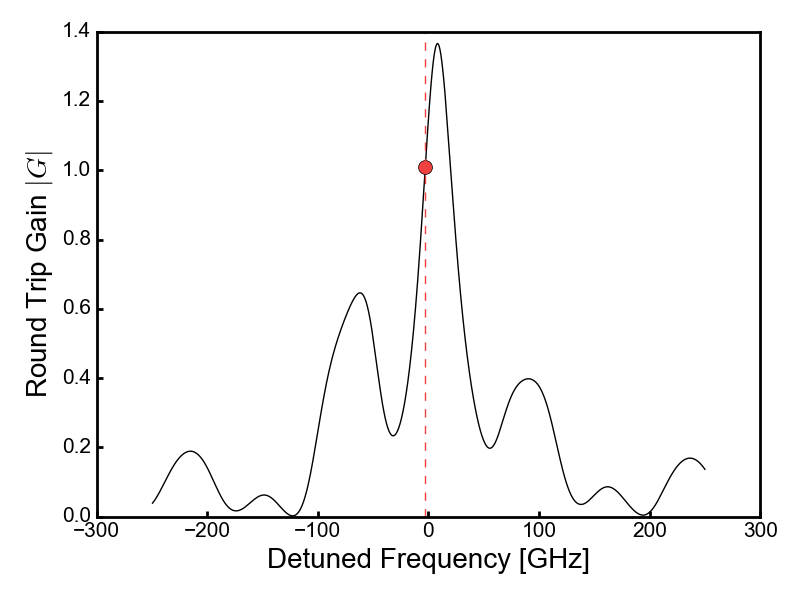
\includegraphics[width=.7\linewidth]{figures/feedback_introduced_detuned_loading_principle.png}
    \caption{Feedback introduced detuned loading condition with respect to the altered round-trip gain. The red marker corresponds to the lasing mode detuend to the longer wavelength side.}
    \label{fig:feedback_introduced_detuned_loading_principle}
\end{figure}

Compare to the round-trip gain without feedback shown in \autoref{fig:detuned_loading_principle}, the detuning at the longer wavelength side shows a deeper slope which permits a larger $B$ parameter, so that an further increase of relaxation oscillation can be achieved according to \autoref{eq:RO_frequency}. 


% Since the incoming feedback acts like a perturbation for the normal laser which introduces the amplitude modulation, the undamped RO can also be called as self-modulation and self-pulsation. The mechanism of self-pulsation is analysed and discussed in \cite{bandelow1993theory} as "dispersive Q-switching". In order to explain the self-pulsations one usually assumes some kind of Q-switching process, where the term Q-switching denotes a switching of the quality-factor of the laser cavity. If an increase of optical power yields a decrease of optical loss (or an increase of optical gain) within the laser, the round trip gain may become larger than unity, yielding an exponential increase of optical power, corresponding to the rising edge of a developing pulse. On the other hand an increased power yields an increasing consumption of carriers untile finally the carrier density is too low to maintain a unity round trip gain and therefore the optical power collapses. A recovery time is required in order to increase the carrier density again until the next pulse develops. The repetition frequency for these pulses is of the same order as the relaxation resonance frequency \cite{petermann2012laser}. The bandwidth enhancement by the self-pulsation effect has beed reported as a clear undamping of the relaxation peak which in some cases ultimately led to self-pulsations at the relaxation frequency is observed in the small signal modulation response of the laser. The increased relaxation frequency and the undamping of the relaxation peak can be utilised in order to achieve higher bandwidth \cite{schatz1996enhanced}.

\subsection{Photon-Photon Resonance}\label{subsec:pp_resonance}
Another approach used to extend the bandwidth takes advantage of the interaction between the lasing mode and an adjacent longitudinal cavity mode. If these two modes can be properly separated and interact due to the applied modulation signal at the gain section, it will introduces a resonance in the direct modulation response at the frequency corresponding to the mode separation \cite{montrosset2014laser}. This resonance is frequently called Photon-Photon resonance (PPR), to distinguish this interaction mechanism respect to the Carrier-Photon resonance (CPR) or Relaxation Oscillation (RO) \cite{montrosset2014laser}. The occurence of the PPR should not be too far away from the relaxation oscillation frequency so that the dip between two peaks will not reach the -3 dB limitation in the modulation response as shown in \autoref{fig:PP_resonance_in_modulation_response}.

\begin{figure}[H]
    \centering
    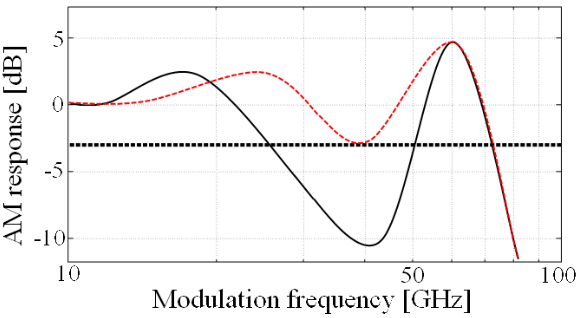
\includegraphics[width=.6\linewidth]{figures/PP_resonance_in_modulation_response.png}
    \caption{Example of modulation responses obtained in a cavity exploiting the PPR effect. The black line indicates a case in which the CPR and the PPR peaks are too far whereas in the case indicated by the red line the modulation bandwidth extension is achieved \cite{montrosset2014laser}.}
    \label{fig:PP_resonance_in_modulation_response}
\end{figure}

The occurence of the adjacent cavity mode has been observed to be closely related to the behavior of the cavity Round-Trip Phase (RTP) function \cite{reithmaier2005modulation}, which refers to the phase factor $\varphi(\omega)$ in \autoref{eq:RTG_RTP}. Calculation for a simplified DBR laser structure is done to illustrate the operation principle of the PPR. By assuming the DBR laser only contains a gain section and grating as in \cite{montrosset2014laser}. Parameters used for this calculation are shown in \autoref{tab:PP_resonance_operation_principle}.

The caculated result is shown in \autoref{fig:PP_resonance_operation_principle},where $f_0$, $f_1$ and $f_B$ denote the frequency of the lasing mode, PPR mode and the freqeuncy corresponding to the Bragg wavelength. The most favorable operation condition is when the lasing mode at $f_0$ operates in the detuned loaidng condition $f_0<f_B$, and a mode with frequency $f_1$ on the same side with respect to the Bragg wavelength is placed on the the longer wavelength side of the Round Trip Gain (RTG) curve. In this mode configuration, the PPR effect can arise due to the coupling between the lasing mode and its adjacent mode \cite{montrosset2014laser}, the corresponding PPR frequency is then the difference between these two modes. In order to generate an adjacent longitudinal cavity mode under feedback, a strong feedback condition is required \cite{mieda2016ultra,ahmed2013enhancing, morthier2000extended,bornholdt200840}, which will form compound cavity modes with the Free Spectral Range (FSR) of the whole cavity considering the laser cavity plus the external feedback section as defined in \autoref{eq:mode_spacing_FSR} \cite{coldren2012diode}
\begin{equation}
    \Delta\nu=\frac{c}{2\qty(n_{gain}L_{gain}+n_{poly}\qty(L_{phase}+L_{grating}+L_{ext}))}
    \label{eq:mode_spacing_FSR}
\end{equation}
this equation is also used as the design guideline in \autoref{sec:design_and_characterization}.

\begin{table}[ht]
    \centering
    \caption{Parameters used for calculating the RTG and RTP for a simplified two-section DBR laser cavity without feedback \cite{montrosset2014laser}.}
    \label{tab:PP_resonance_operation_principle}
    \begin{tabular}{@{}lll@{}}
    \toprule
    Symbol    & Description                  & Value        \\ \midrule
    $L_A$     & Active region length         & 140 $\mu m$  \\
    $L_G$     & Grating region length        & 780 $\mu m$  \\
    $\kappa$  & Grating coupling coefficient & 20 $cm^{-1}$ \\
    $n_{eff}$ & Effective refractive index   & 3.7          \\
    $R_R$     & Right side reflectivity      & 0            \\
    $R_L$     & Left side reflectivity       & 0.32         \\ \bottomrule
    \end{tabular}
\end{table}

\begin{figure}[ht]
    \centering
    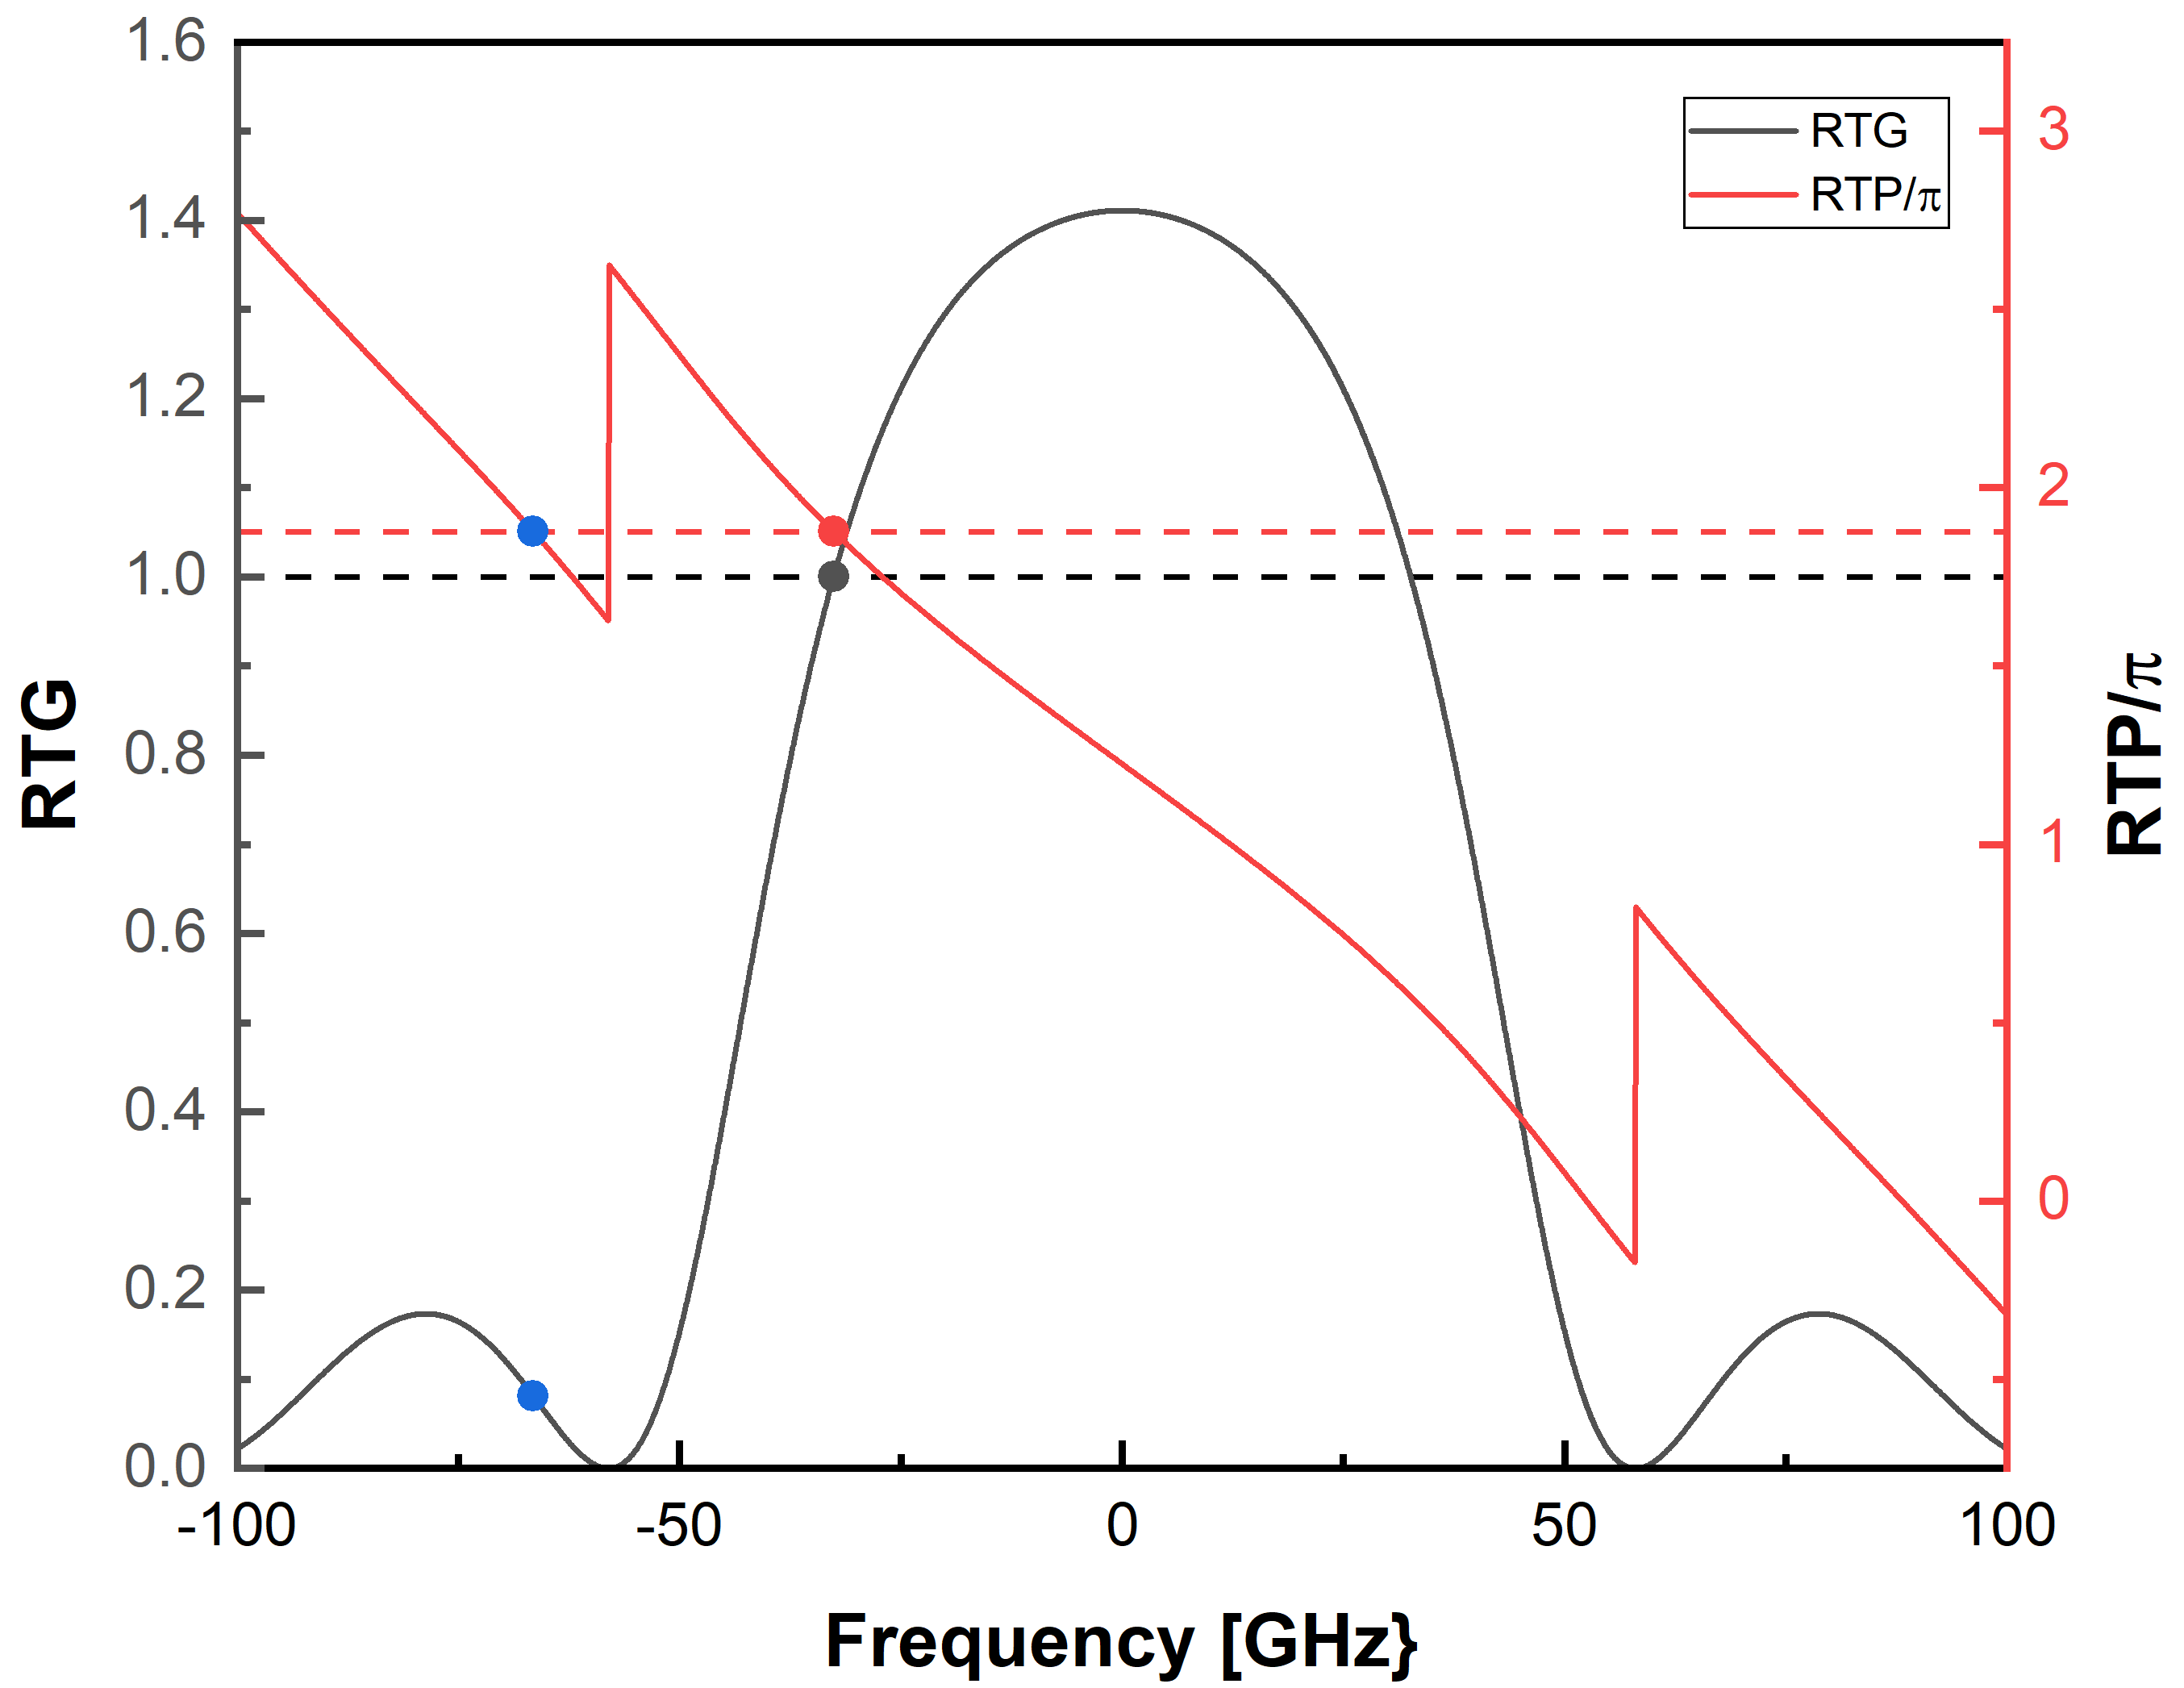
\includegraphics[width=.7\linewidth]{figures/PP_resonance_operation_principle.png}
    \caption{Round trip gain (RTG, grey curve) and phase (RTP, red curve) functions calculated for a simplified two-section DBR laser without feedback. The grey and red marker represent the lasing mode at frequency $f_0$ on the corresponding RTG and RTP curve, the blue marker indicates the PPR mode at freqeuncy $f_1$.}
    \label{fig:PP_resonance_operation_principle}
\end{figure}

\chapter{Tunable Laser with Feedback from the Output Waveguide Facet}\label{ch:Laser_with_feedback_from_facet}
Characterization of the hybrid polymer-based tunbale DBR laser linewidth, bandwidth and $\alpha$ parameter are measured with and without feedback from the output facet. This has been done by measuring with a cleaved fiber and using index-matching oil (case without optical feedback), and with a lensed fiber at the output and without index matching oil (case with feedback from the output waveguide facet), the two measurement configurations are shown in \autoref{fig:coupling}. Principle of each measurement will be introduced and the results will be compared in the following sections.

\begin{figure}[ht]
    \centering
    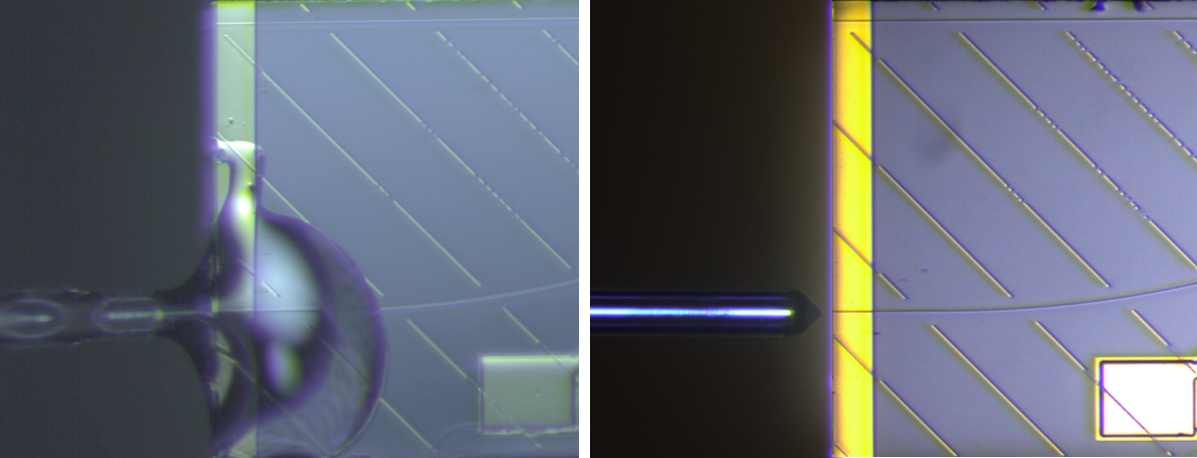
\includegraphics[width=\linewidth]{figures/coupling.png}
    \caption{(a) Measuring with cleaved fiber and using index-matching oil (case without optical feedback), (b) measuring with lensed fiber at the output and without index matching oil (case with feedback from the output waveguide facet).}
    \label{fig:coupling}
\end{figure}

\section{Effect of Feedback in the Lasing Spectrum}\label{sec:feedback_influenced_lasing_spectral_behavior}
With the effect of feedback, modes formed in the external feedback section between the grating reflector and the external reflector appear along with the modes in the laser cavity, they have different mode spacing because of their different section length, which is given by \cite{coldren2012diode}
\begin{equation}
    \Delta\nu_{cavity}=\frac{c}{2(n_{gain}L_{gain}+n_{poly}L_{poly})}
    \label{eq:mode_spacing_laser_cavity}
\end{equation}
\begin{equation}
    \Delta\nu_{ext}=\frac{c}{2n_{poly}L_{ext}}
    \label{eq:mode_spacing_external}
\end{equation}
where $L_{poly}$ and $L_{ext}$ follow the definition in \autoref{sec:model_laser}.

The spacing betwee the laser cavity mode and the mode formed in the external feedback section will change by tuning the phase through the increasing current, which in turn shifts the laser cavity modes towards the shorter wavelength side. The mode have the lowest cavity loss (highest intensiy) overlaping with the grating response will become the lasing mode. The principle of wavelength tuning is presented in \autoref{fig:cavity_modes_and_ext_modes_model}.

\begin{figure}[ht]
    \centering
    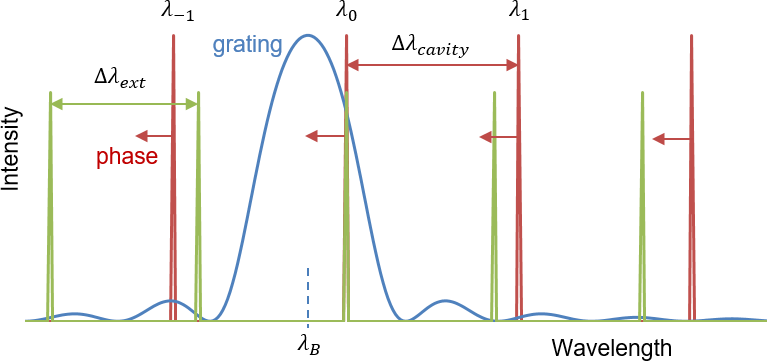
\includegraphics[width=.7\linewidth]{figures/cavity_modes_and_ext_modes_model.png}
    \caption{Principle of phase tuning in tunable DBR laser. Red and green curves represent the mode of the laser cavity and external feedback section respectively, and the blue curve is the grating response. }
    \label{fig:cavity_modes_and_ext_modes_model}
\end{figure}

The red and green curves in \autoref{fig:cavity_modes_and_ext_modes_model} represent the laser cavity mode and the mode in the external feedback section, and the blue curve is the grating response. The different intensity considers that the feedback power is less than the output power. $\lambda_0$ is the lasing mode, $\lambda_{-1}$ and $\lambda_{1}$ are its adjacent modes. $\lambda_B$ is the Bragg wavelength which indicates the center of the grating response. $\Delta\lambda_{cavity}$ and $\Delta\lambda_{ext}$ are the mode spacing of the laser cavity and the external feedback section. The red arrow indicates the phase shifts the cavity modes toward the shorter wavelength through the increasing phase current. Besides the lasing mode, the interaction between the laser cavity mode and the mode formed in the external cavity is expected to appear at the grating side bands which will alter the lasing spectrum.

Examing the lasing spectrum for laser with feedback was done by measuring the central wavelength and Side-Mode-Suppression-Ratio (SMSR) simultaneously and then compared with the same measurement for laser without feedback. The measurements were done by fixing the gain section current at $I_{gain}=80 \ mA$, grating section current at $I_{grating}=15 \ mA$ and scanning the phase section from $4.5 \ mA$ to $30 \ mA$ with the step of $0.5 \ mA$, the results are shown in \autoref{fig:OSA_and_SMSR} and examples of spetra are shown in \autoref{fig:spectra_lensed_4621}. 
% Due to the hysteresis effect the laser wavelength has a little shift under these two configurations, e.g. the mode hopping point in \autoref{fig:OSA_and_SMSR} a) appears at index 51 and the corresponding point in \autoref{fig:OSA_and_SMSR} (b) is at index 48.

\begin{figure}[ht]
    \centering
    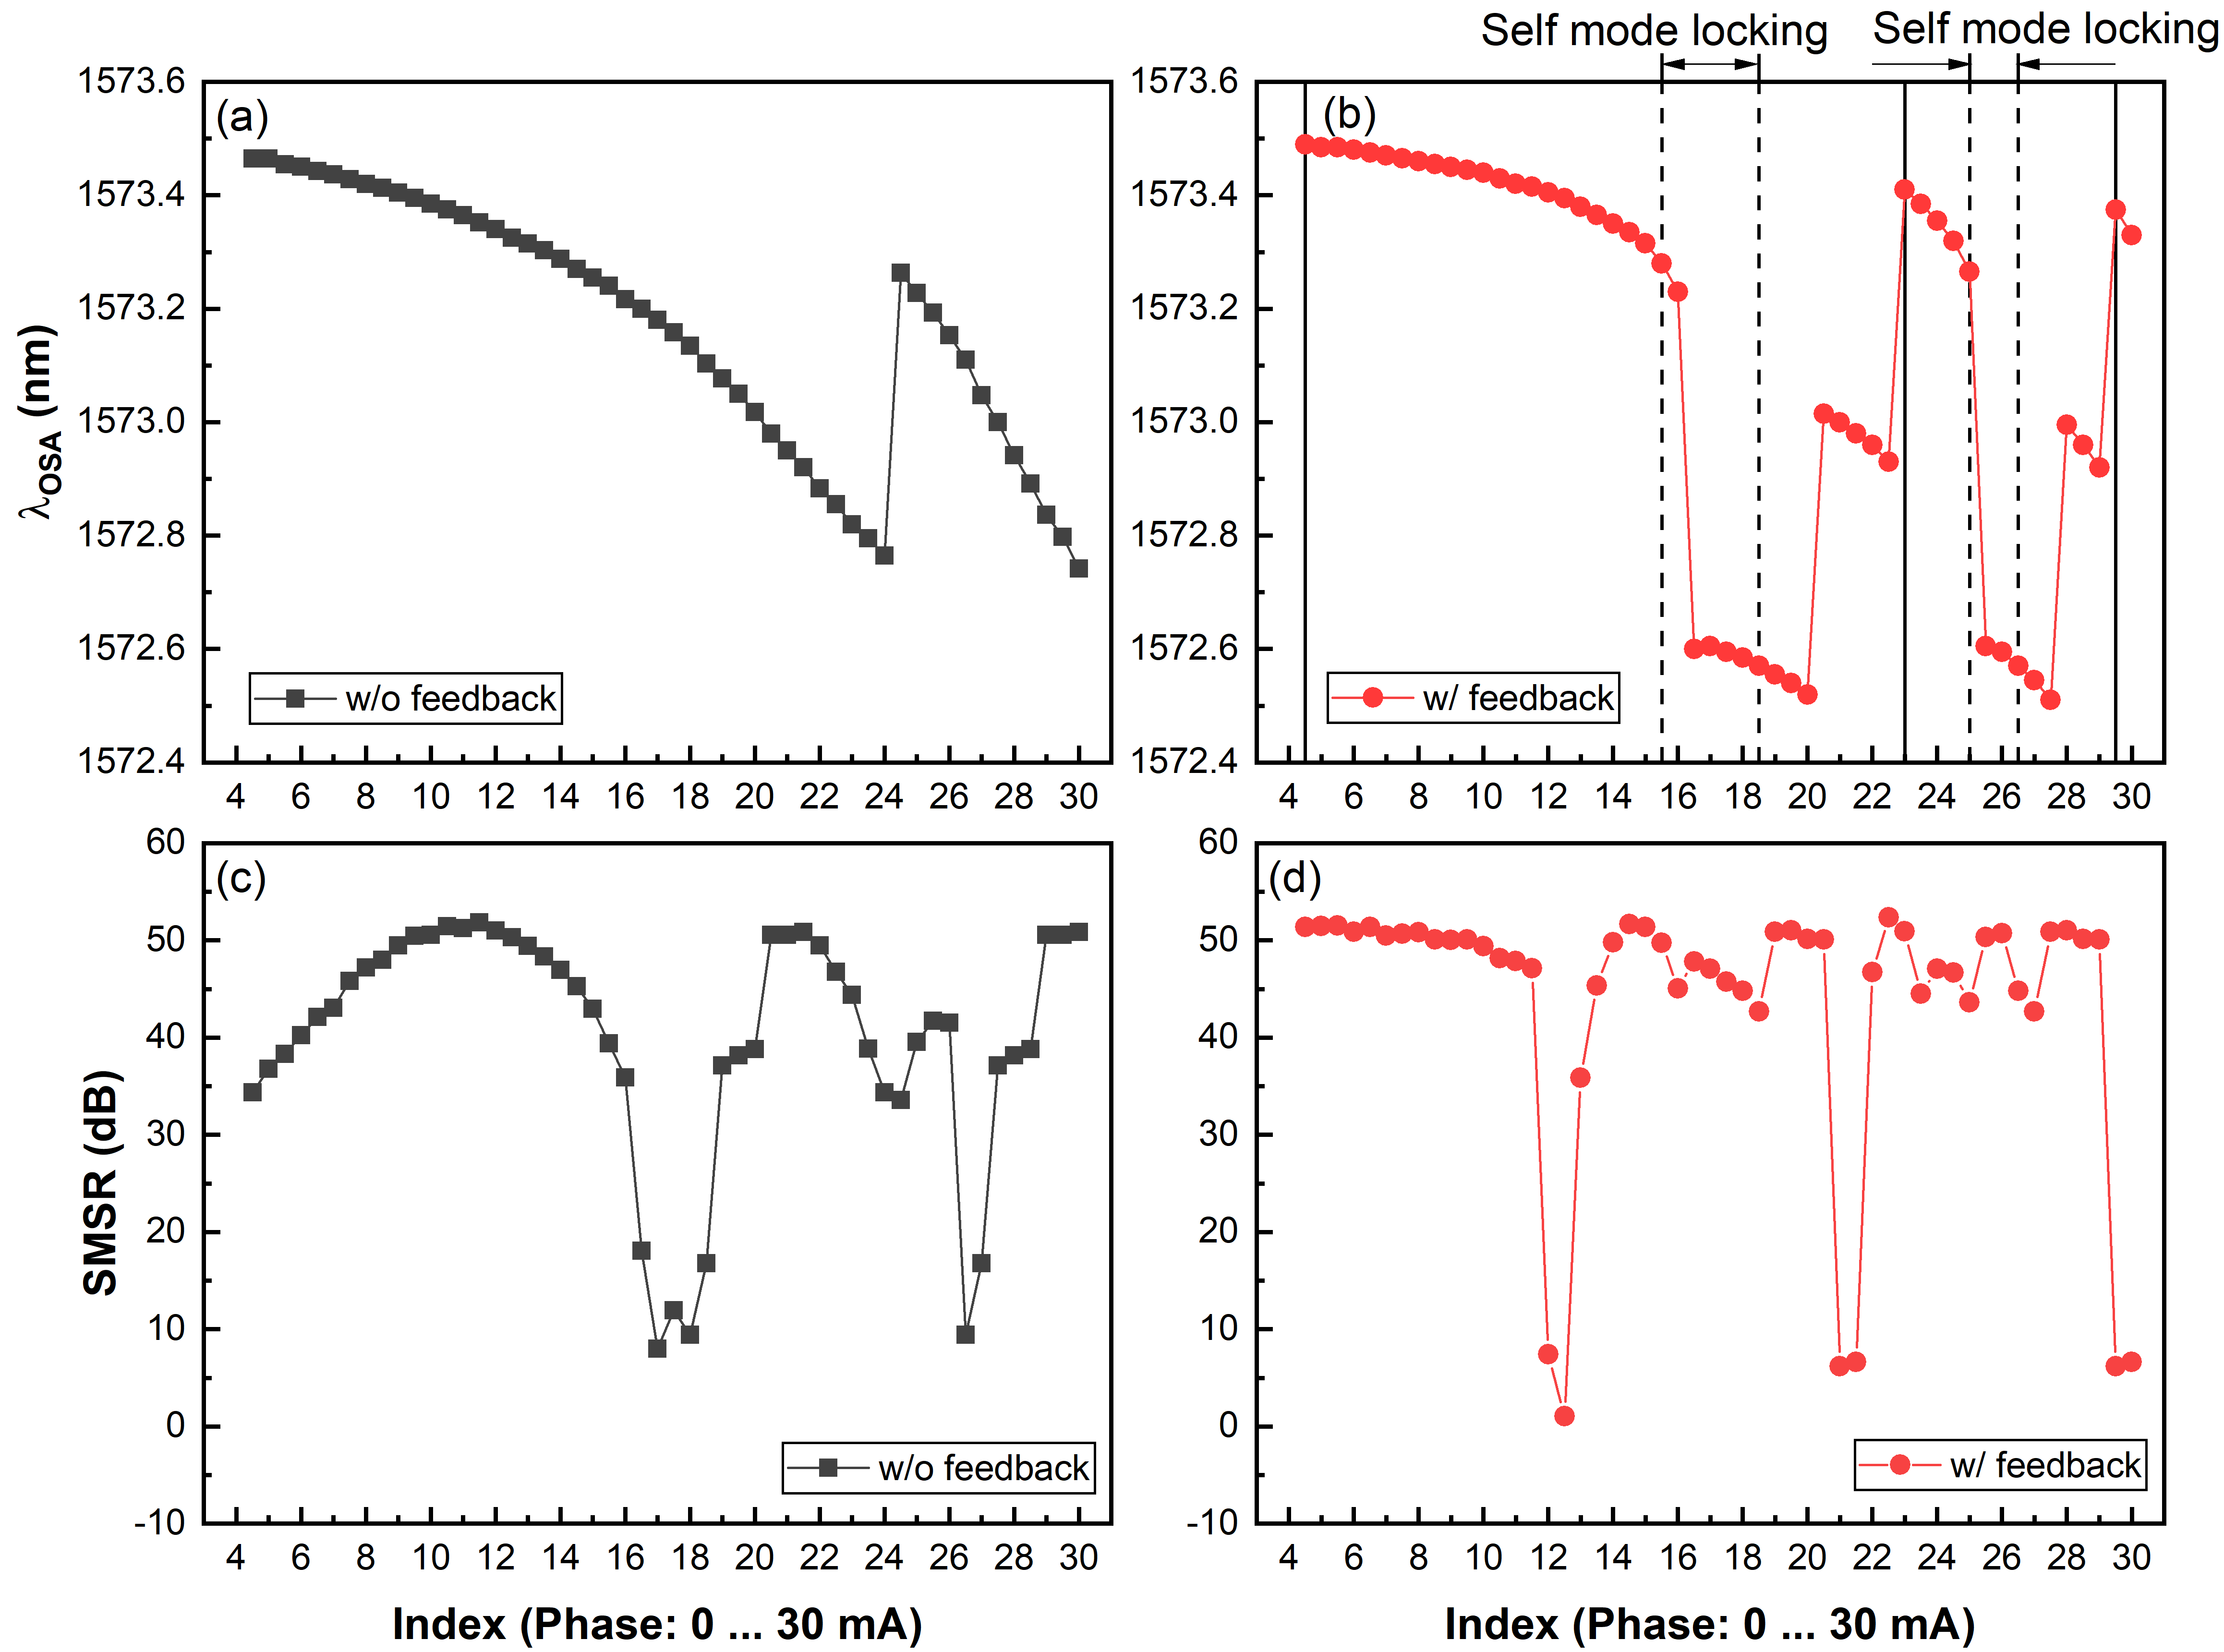
\includegraphics[width=\linewidth]{figures/OSA_and_SMSR.png}
    \caption{Comparison of wavelength scanning (a), (b) and SMSR (c), (d) for tunbale DBR laser with feedback (red circled curve) and without feedback (black squared curve).}
    \label{fig:OSA_and_SMSR}
\end{figure}

\begin{figure}[H]
    \centering
    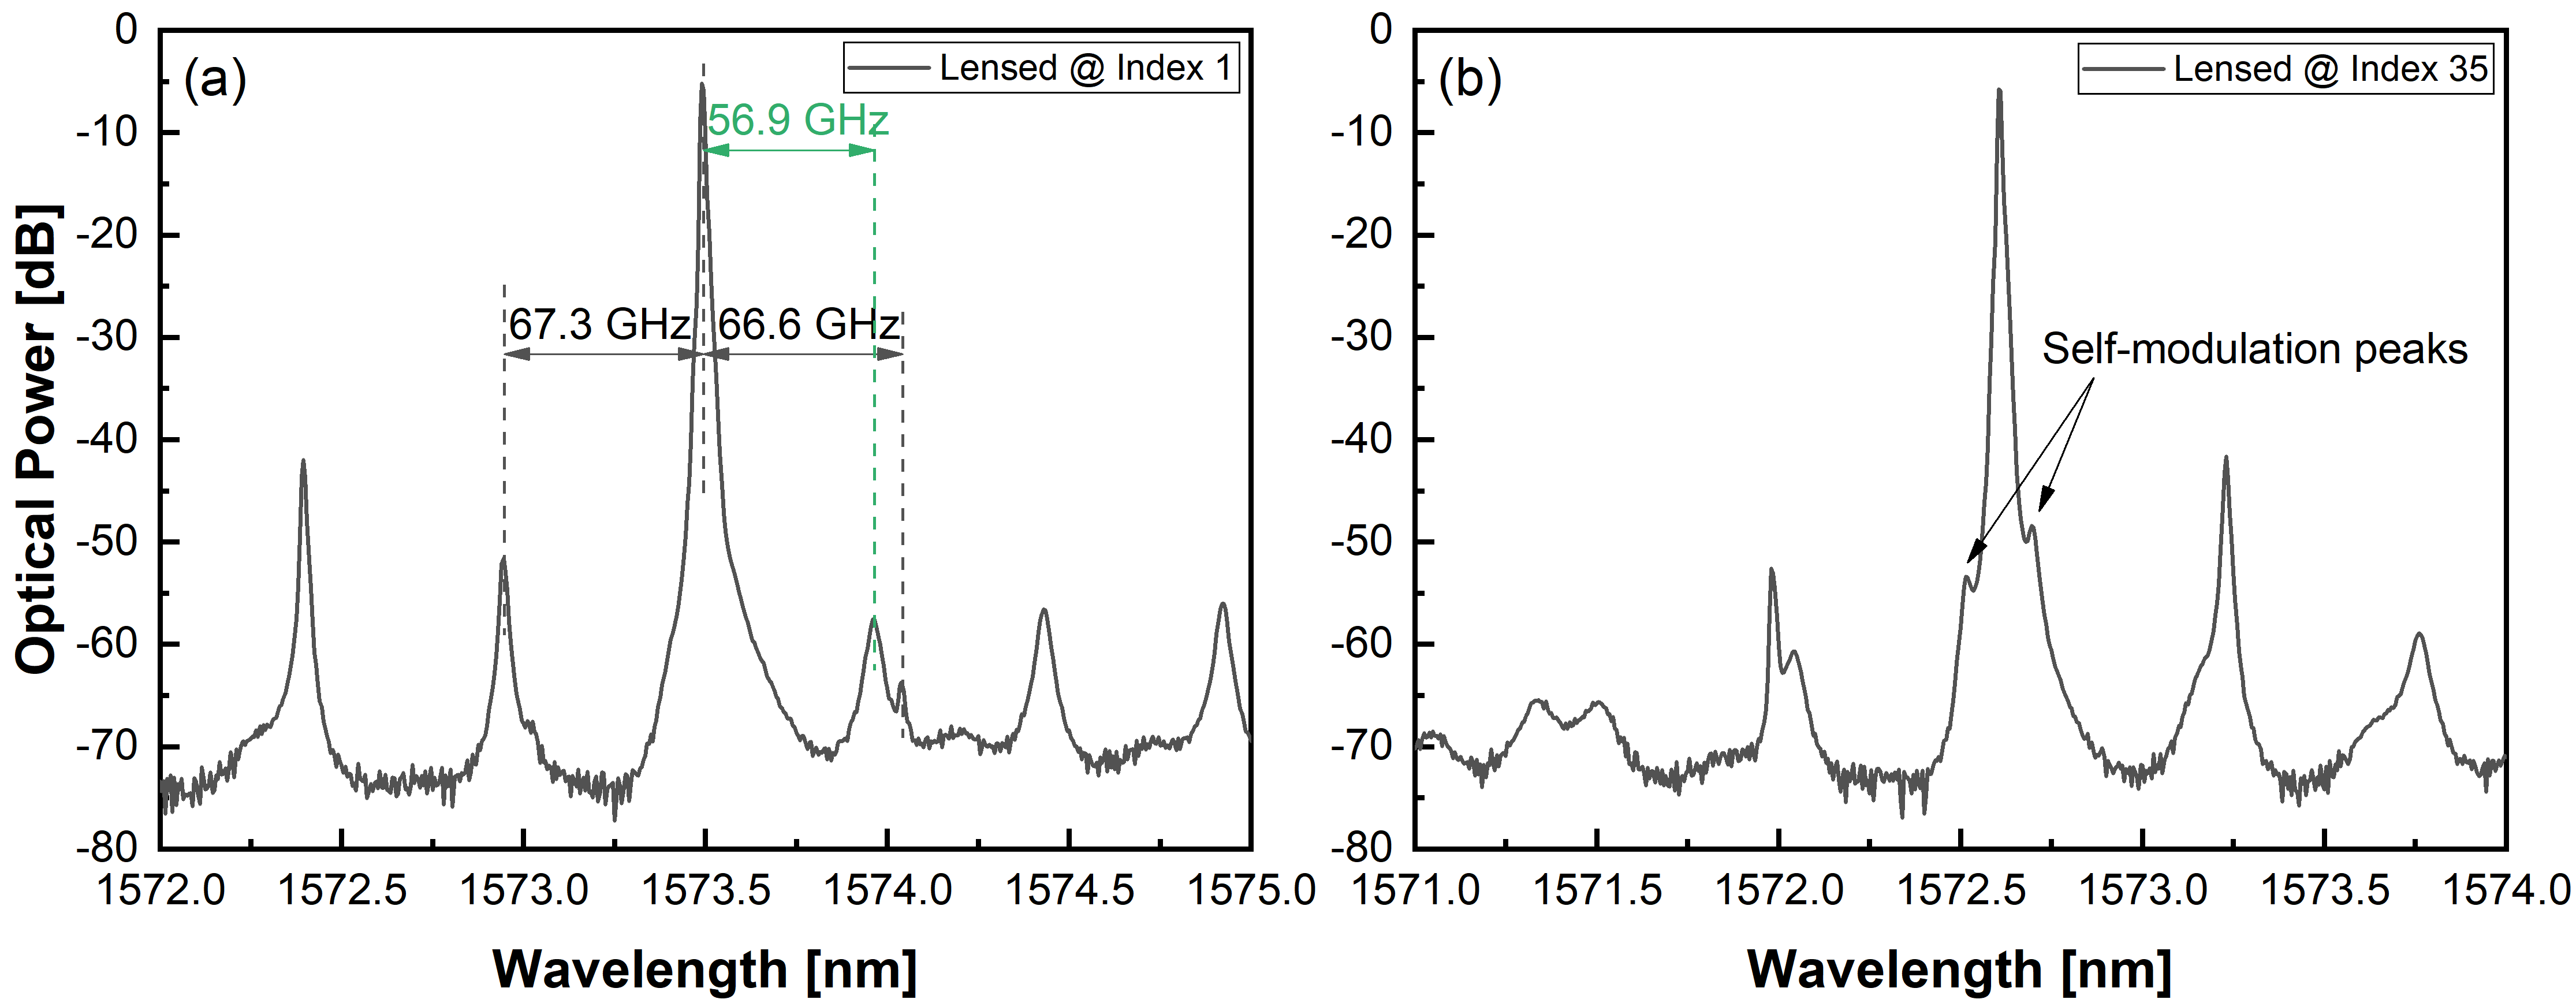
\includegraphics[width=\linewidth]{figures/spectra_lensed_4621.png}
    \caption{Example of observed spectra for different phase current. (a) Green dashed line indicates the mode spacing between the main mode and the first side mode on the right, which corresponds to the laser cavity mode spacing $\Delta\nu_{ext}=56.35 \ GHz$, black dashed line indicates the mode spacing correspoinds to the external feedback section $\Delta\nu_{cavity}=67.04 \ GHz$, (b) occurence of the self-modulation peaks on both sides of the main mode are pointed with black arrows.}
    \label{fig:spectra_lensed_4621}
\end{figure}

Compare to the wavelength shifting behavior for laser without feedback in \autoref{fig:OSA_and_SMSR} (a), additional hopping behavior in \autoref{fig:OSA_and_SMSR} (b) appears due to the feedback effect. Using the parameters in \autoref{tab:F_reduction_factor} along with the external cavity formed between the end of the grating and the output waveguide facet with length of $L_{ext}=1473.36 \ \mu m$, mode spacing for laser cavity and external feedback section were calculated as $\Delta\nu_{cavity}=67.04 \ GHz$ and $\Delta\nu_{ext}=56.35 \ GHz$ respectively. As seen from \autoref{fig:spectra_lensed_4621} (a), the laser initially operates with the side mode spacing corresponds to the external feedback section, it is because with the feedback from the output waveguide facet $R_{ext}=0.035$, the laser operates in the relative strong feedback region with $C=1.69$ calculated by \autoref{eq:C}. While shifting the phase current, small side peaks which relates to the behavior of self-modulation \cite{broom1969self, broom1970microwave} start to appear beside the main mode as shown in and \autoref{fig:spectra_lensed_4621} (b).

Regarding to the cavity mode shifting principle, the occurence of the self modulation peaks can be understood as a self mode locking behavior between the laser cavity mode and the mode in the external feedback section, which is reported in \cite{tager1994high}. In this case, this term is used to name the region where these effects occurs, as shown in \autoref{fig:OSA_and_SMSR} (b), to seperate with the other lasing conditions along the phase shifting current.

Further understanding of the self-modulation peaks introduced by feedback was done by examing the lasing spectrum while tuing the wavelength through the phase current, the result is shown in \autoref{fig:undamped_RO_measurement}.

\begin{figure}[ht]
    \centering
    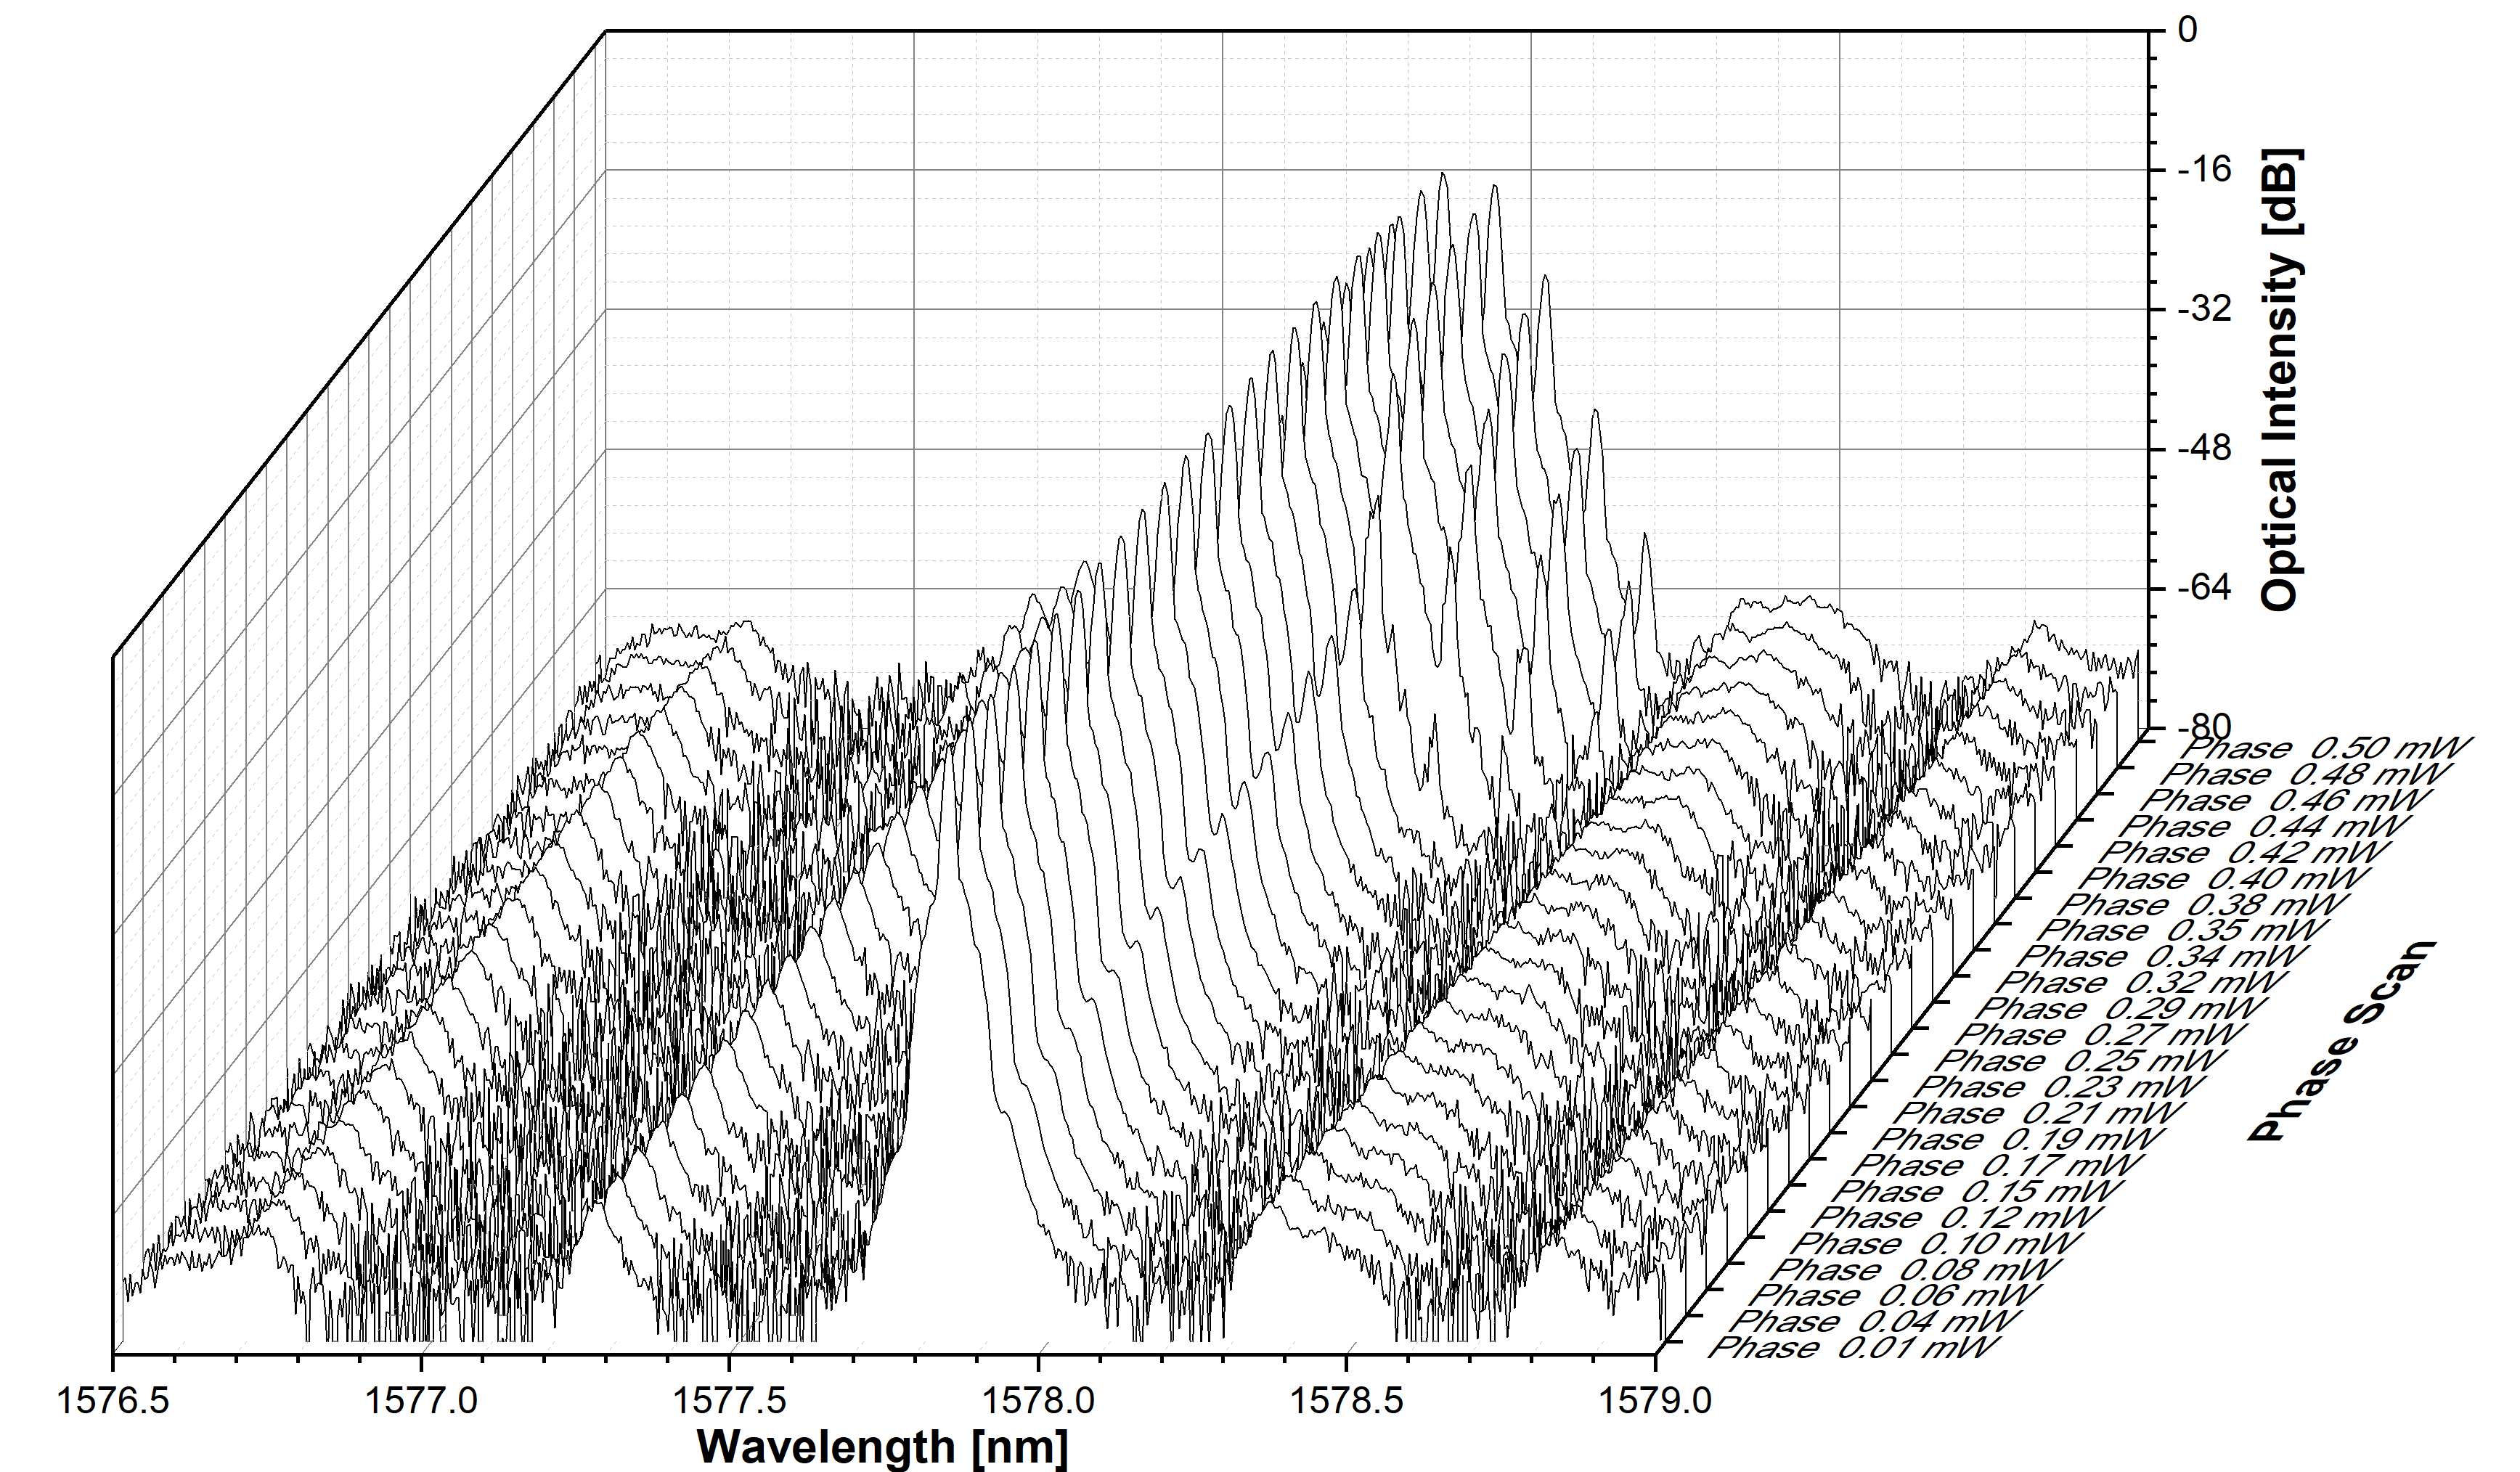
\includegraphics[width=\linewidth]{figures/Undamped_RO_phase_scan_grating_4621.png}
    \caption{Phase scan of the tunable DBR laser spectra with feedback from output waveguide facet. The side peaks of undamped RO start to appear, increase their intensity and shift toward the main peak. While the applied phase current keeps increasing, more peaks develop until the laser shift to another mode and operates as stable single mode lasing again.}
    \label{fig:undamped_RO_phase_scan}
\end{figure}

Small satellite peaks in \autoref{fig:undamped_RO_phase_scan} first show up with low phase current, then slowly increase their intensity and move towards the main peak, followed by more satellite peaks appearing which leads to the undamped relaxation oscillation \cite{lenstra1985coherence, bauer2004nonlinear, soriano2013complex} behavior where the mode spacing between the satellite peaks correspoinds to the relaxation oscillation frequency \cite{petermann2012laser}.

The feedback introduced undamped relaxation oscillation behavior \cite{lenstra1985coherence, bauer2004nonlinear, soriano2013complex} can be understood as the incoming feedback acts like a perturbation for the laser cavity and introduces the amplitude modulation which is named as self-modulation \cite{broom1969self, broom1970microwave} or self-pulsation \cite{petermann2012laser}. It can be explained that the increase of optical power from the feedback yields an increase of optical gain within the laser so that the roud-trip gain reaches over one and optical power exponentialy increases. On the other hand, an increased power yields an increasing consumption of carriers until the carrier density is too low to maintain a unity roud trip gain and therefore the optical power collapses. A recovery time is required in order to increase the carrier density again until the next pulse develops. The repetition frequency for these pulses is of the same order as the relaxation resonance frequency \cite{petermann2012laser}.

% The undamped relaxation oscillation occurs for the appropriate combinations of feedback phase and strength as shown in \autoref{fig:undamped_RO_phase_scan}. 

\section{Measurement of Feedback Effects on Linewidth}\label{sec:linewidth_measurement}
Feedback influenced laser linewidth is measured and compared with the laser linewidth without feedback condition. Self-homodyne method is used and the principle can be described mathematically as a single-delay autocorrelation, which is shown in \autoref{fig:self-homodyne}, the optical spectrum at $f_0$ autocorrelates with the delayed version of itself to produce a time-fluctuating spectrum, whose detected voltage has a power spectrum centered at zero frequency. For the case of a laser with Lorentzian lineshape, the half-width of the detected spectrum is equal to the linewidth of the laser.
\begin{figure}[ht]
    \centering
    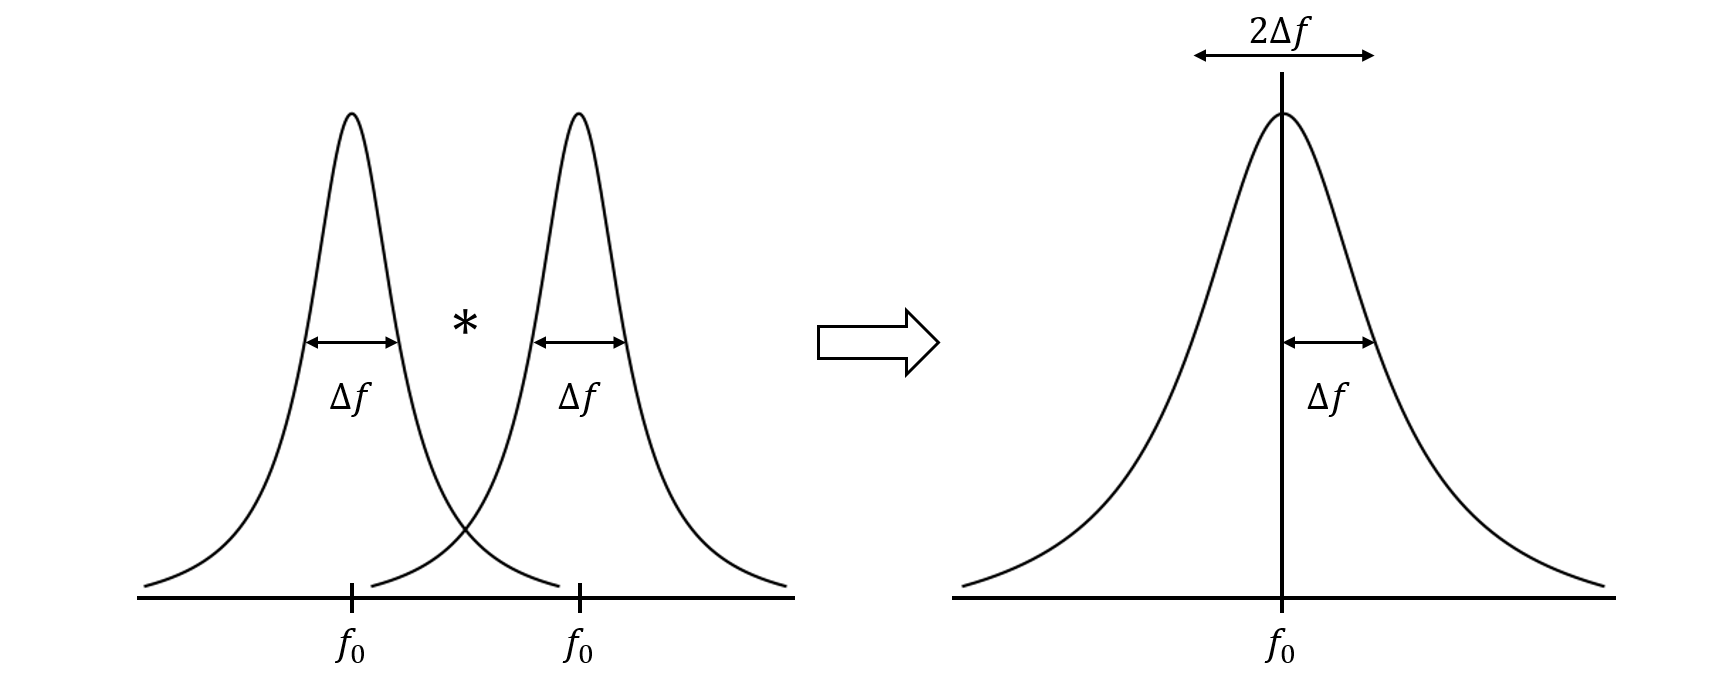
\includegraphics[width=.8\linewidth]{figures/self-homodyne.png}
    \caption{Linewidth of a DBR laser using the self-homodyne technique. The optical spectrum at $f_0$ autocorrelates with the delayed version of itself to produce a time-fluctuating spectrum, whose detected voltage has a power spectrum centered at zero frequency, the half-width of the detected spectrum is equal to the linewidth of the laser.}
    \label{fig:self-homodyne}
\end{figure}

The self-homodyne measurement set-up is shown in \autoref{fig:self-homodyne_setup}. The input directional coupler of the interferometer splits the light from the laser into two paths. One path is delayed in order to decorrelate the combinning signals, $P_1$ and $P_2$. The output coupler combines the two signals, which are then mixed at the photodectector of the lightwave signal analyzer.  The homodyne power spectrum is then observed on the analyzer from which the Lorentzian linewidth is measured by placing a marker at the half power frequency.
\begin{figure}[ht]
    \centering
    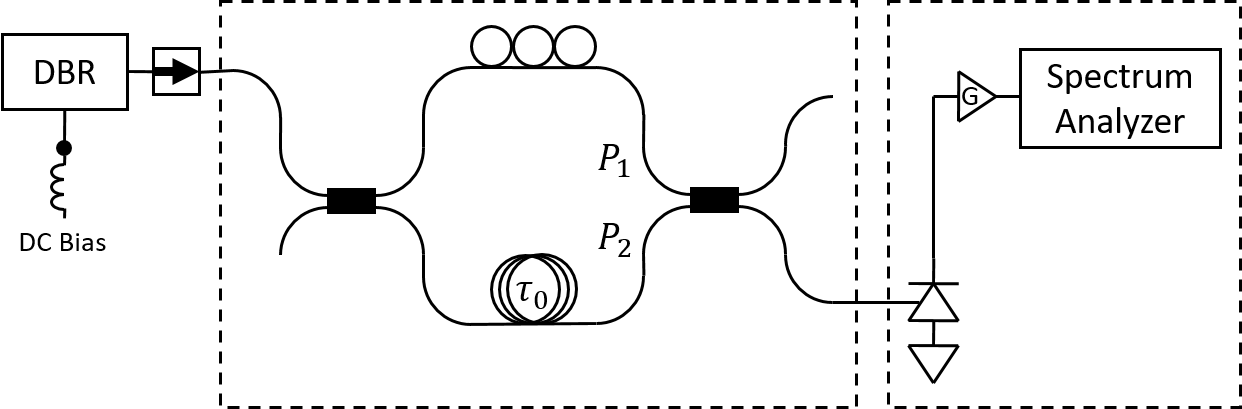
\includegraphics[width=.8\linewidth]{figures/self-homodyne_setup.png}
    \caption{Schematic set-up for self-homodyne linewidth measurement.}
    \label{fig:self-homodyne_setup}
\end{figure}

The results of linewidth measurement are shown in \autoref{fig:LB_Cleaved_and_Lensed}. The laser linwidth under feedback shows a more stable transition and become narrower than the case without feedback. It is due to the reason that the external refelctor formed by the polymer/air interface with $R_{ext}=0.035$ leads to $C=1.69$, it is considered to be in the relative strong feedback region. In such case, the practical formula for linewidth reduction factor $F^2$ \autoref{eq:F_strong_feedback} has to be considered. The comparison for the lowerest linewidth for two configurations, along with the theoretical predcition, is shown in \autoref{tab:linewidth_comparison}.

\begin{figure}[H]
    \centering
    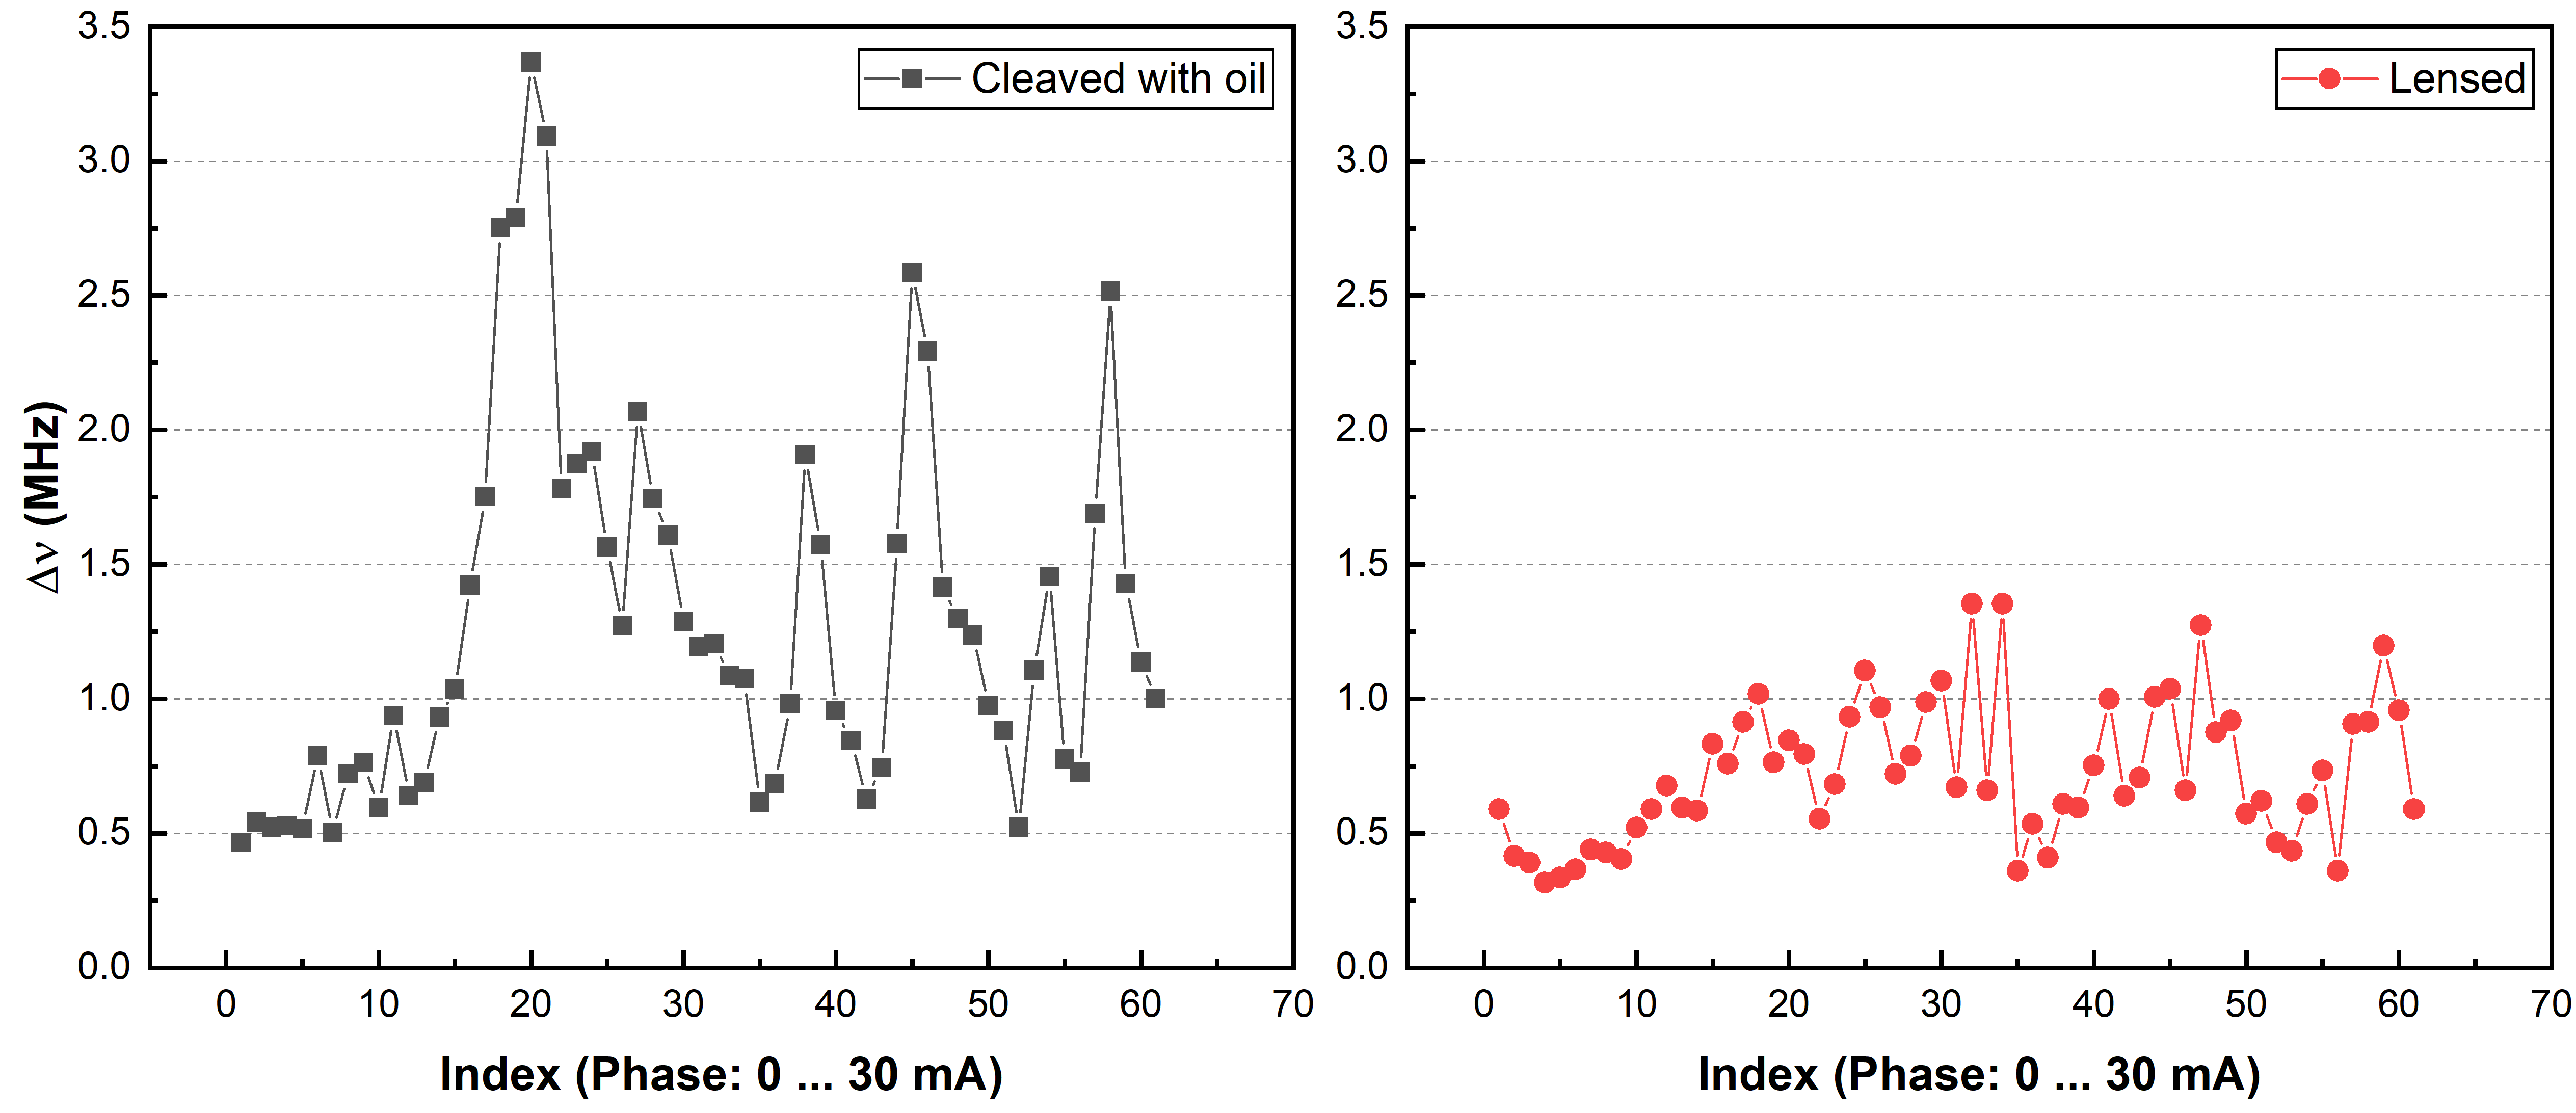
\includegraphics[width=\linewidth]{figures/LB_Cleaved_and_Lensed.png}
    \caption{(a) The laser linewidth without feedback from the output waveguide facet (b) laser linewidth with feedback from the output waveguide facet, it appears to be more stable compare to the laser without feedback. The achieved lowest linewidth point are pointed with black arrow in each case.}
    \label{fig:LB_Cleaved_and_Lensed}
\end{figure}

% \begin{table}[ht]
%     \centering
%     \caption{Comparison between the linewidth reduction value achieved by laser w/ and w/o feedback and the predicated reduction value.}
%     \begin{tabular}{@{}lllll@{}}
%     \toprule
%                                              & Cleaved with oil & Lensed          & Reduction & \multicolumn{1}{c}{\begin{tabular}[c]{@{}c@{}}Reduction\\ (Predicated)\end{tabular}} \\ \midrule
%     \multicolumn{1}{c}{$\Delta \nu \ (MHz)$} & 0.522 @ Index 52 & 0.317 @ Index 4 & 1.647     & 1.11                                                                                 \\ \bottomrule
%     \end{tabular}
%     \label{tab:linewidth_comparison}
% \end{table}

\begin{table}[ht]
    \centering
    \caption{Comparison between the linewidth reduction value achieved by laser w/ and w/o feedback and the predicated reduction value.}
    \label{tab:linewidth_comparison}
    \begin{tabular}{@{}lllll@{}}
    \toprule
    \multirow{2}{*}{} & \multirow{2}{*}{w/o feedback} & \multirow{2}{*}{w/ feedback} & \multicolumn{2}{c}{Linewdith reduction factor $F^2$} \\
                      &                               &                              & Measured               & Predicated               \\ \midrule
    $\Delta\nu \ [MHz]$ & 0.522 @ $20.5 \ mA$              & 0.360 @ $12 \ mA$              & 1.45                     & 1.11                     \\ \bottomrule
    \end{tabular}
\end{table}

The difference between the measured and predicated value may comes from the assumption considered in \autoref{eq:F_strong_feedback}, since it mainly considers the ratio between the length of external feedback section and the laser cavity, which is mainly denoted as $A$ paramter in the defination of $F$ factor in \autoref{eq:F_factor}. The contribution from the frequency dependence of the reflectance parameter $B$ is not included which may further increase the predicated linewidth reduction factor.

% \section{Relative Intensity Noise (RIN) Measurement}\label{sec:RIN_measurement}
% The measurement of relative intensity noise (RIN) describes the laser’s maximum available range for signal modulation and serves as a quality indicator of laser devices. RIN is defined as the ratio of the mean-square optical intensity noise to the square of the average optical power \cite{petermann2012laser}
% \begin{equation}
%     RIN=\frac{\langle \Delta P \rangle ^2}{\langle P \rangle ^2}dB/Hz
% \label{RIN_1}
% \end{equation}
% where $\langle \Delta P \rangle ^2$ is the mean-square optical intensity fluctuations (in a 1-Hz bandwidth) at a specified frequency, and $\langle P \rangle$ is the mean optical power.

% In order to measure the RIN, the optical power is converted to a current after the receiving photodiode and the ratio of optical powers squared is equivalent to the ratio of the detected electrical powers. Thus, $RIN$ can be expressed in terms of detected electrical powers. \autoref{RIN_1} can be rewritten as
% \begin{equation}
%     RIN=\frac{N_{elec}}{P_{avg}(elec)} \ dB/Hz
%     \label{eq:RIN_2}
% \end{equation}
% where $N_{elec}$ is the power-spectral density of the photocurrent at a specified frequency, and $P_{avg}(elec)$ is the average power of the photocurrent.

% The noise at the receiver output results from three fundamental contributions: laser intensity noise primarily due to spontaneous light emissions; thermal noise from the electronics; and photonic shot noise. Since the photonic shot noise and the receiver thermal noise are not included in the definition of $N_{elec}$, they have to be subtracted from the measured $RIN$ results
% \begin{equation}
%     N_{laser}=N_{elec}-N_{shot}-N_{thermal} \ W/Hz
%     \label{eq:RIN_3}
% \end{equation}
% By using \autoref{eq:RIN_2} and \autoref{eq:RIN_3}, the value of $RIN_{laser}$ can be determined
% \begin{equation}
%     RIN_{laser}=RIN(measured)-\frac{2e}{I_{avg}}-\frac{N_{thermal}}{P_{avg}(elec)}
%     \label{eq:RIN_4}
% \end{equation}
% where $e$ is the elementary charge, $I_{avg}$ denotes the detected average photocurrent, $N_{thermal}$ is the measured noise floor of the lightwave signal analyzer in a 1-Hz bandwidth.

% The RIN comparison for the two configurations are shown in \autoref{fig:RIN_cleaved_and_lensed}. The RIN value for laser w/o feedback ranges from $-144.086 \ dB/Hz$ to $-141.507 \ dB/Hz$ while for lase with feedback it has two parts: without the spikes it ranges from $-146.283 \ dB/Hz$ to $-140.216 \ dB/Hz$, which is lower than the case without feedback; the spikes appear in \autoref{fig:RIN_cleaved_and_lensed} (b) are corresponding to the additional mode hopping behavior in \autoref{fig:OSA_and_SMSR} (b), which indicates the appearing of the undamped RO, will increase the RIN value.

% \begin{figure}[ht]
%     \centering
%     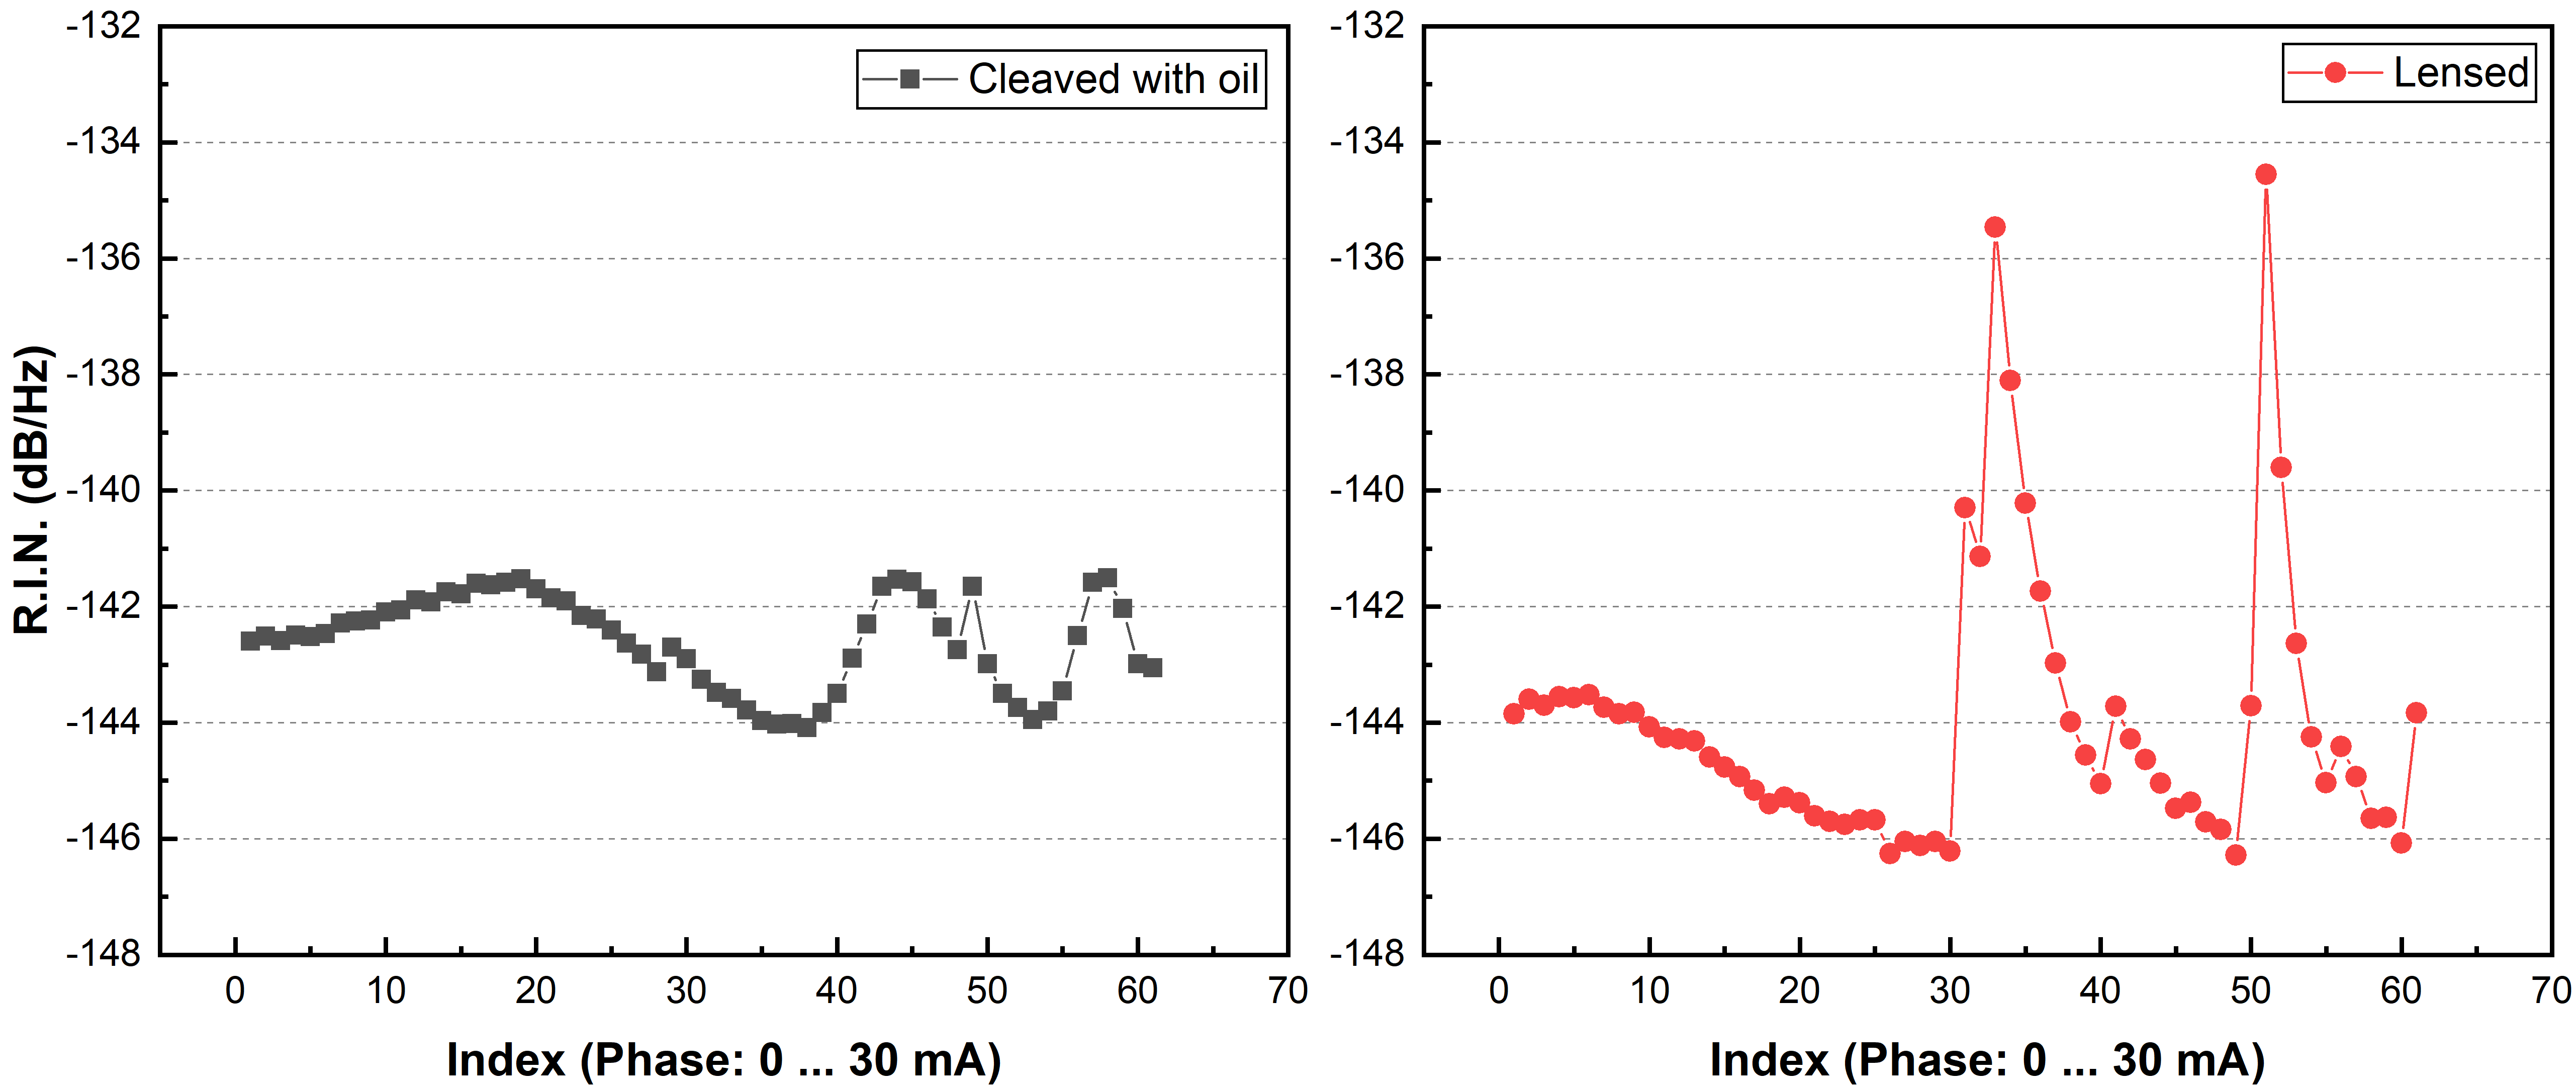
\includegraphics[width=\linewidth]{figures/RIN_cleaved_and_lensed.png}
%     \caption{Comparison of the RIN value for laser w/ and w/o feedback. (a) Laser with feedback, (b) laser without feedback, the spikes indicate the appearing of the undamped RO, which increase the RIN significantly.}
%     \label{fig:RIN_cleaved_and_lensed}
% \end{figure}

\section{Measurement of Feedback Effects on Bandwidth}\label{sec:bandwidth_measurement}
Bandwidth for laser with feedback is compared with the case without feedback by the measurement of small signal modulation. Detuned loading condition achieved in both cases are presented. Photon-photon resonance is not observed because the feedback is not strong enough to form counpound cavity modes.

The frequency response of a laser transmitter under small signal modulation is found by the usual assumption of a harmonic current modulation superimposed on a constant bias above threshold \cite{tucker1985high}. The modulation bandwidth $f_{3dB}$ is a measure of the maximum modulation ability in semiconductor lasers through the injection current. It is usually defined as the frequency at which the modulation response has dropped by $3 \ dB$ relative to its zero freqeuncy value \cite{ohtsubo2012semiconductor, agrawal2013semiconductor}. The characteristics of the small signal modulation in a normal laser are mainly determined by the relaxation oscillation frequency $f_r$, which indicated by the position of the peak in the modulation response. 

The comparison of bandwidth for the polymer-based tunbale laser was characterized at different gain current value. It was done by scanning through the gain current from $40 \ mA$ to $100 \ mA$ with a step of $5 \ mA$ and is presented in \autoref{fig:bandwidth_gain_scan_cleaved_and_lensed}. 

% \begin{figure}[ht]
%     \centering
%     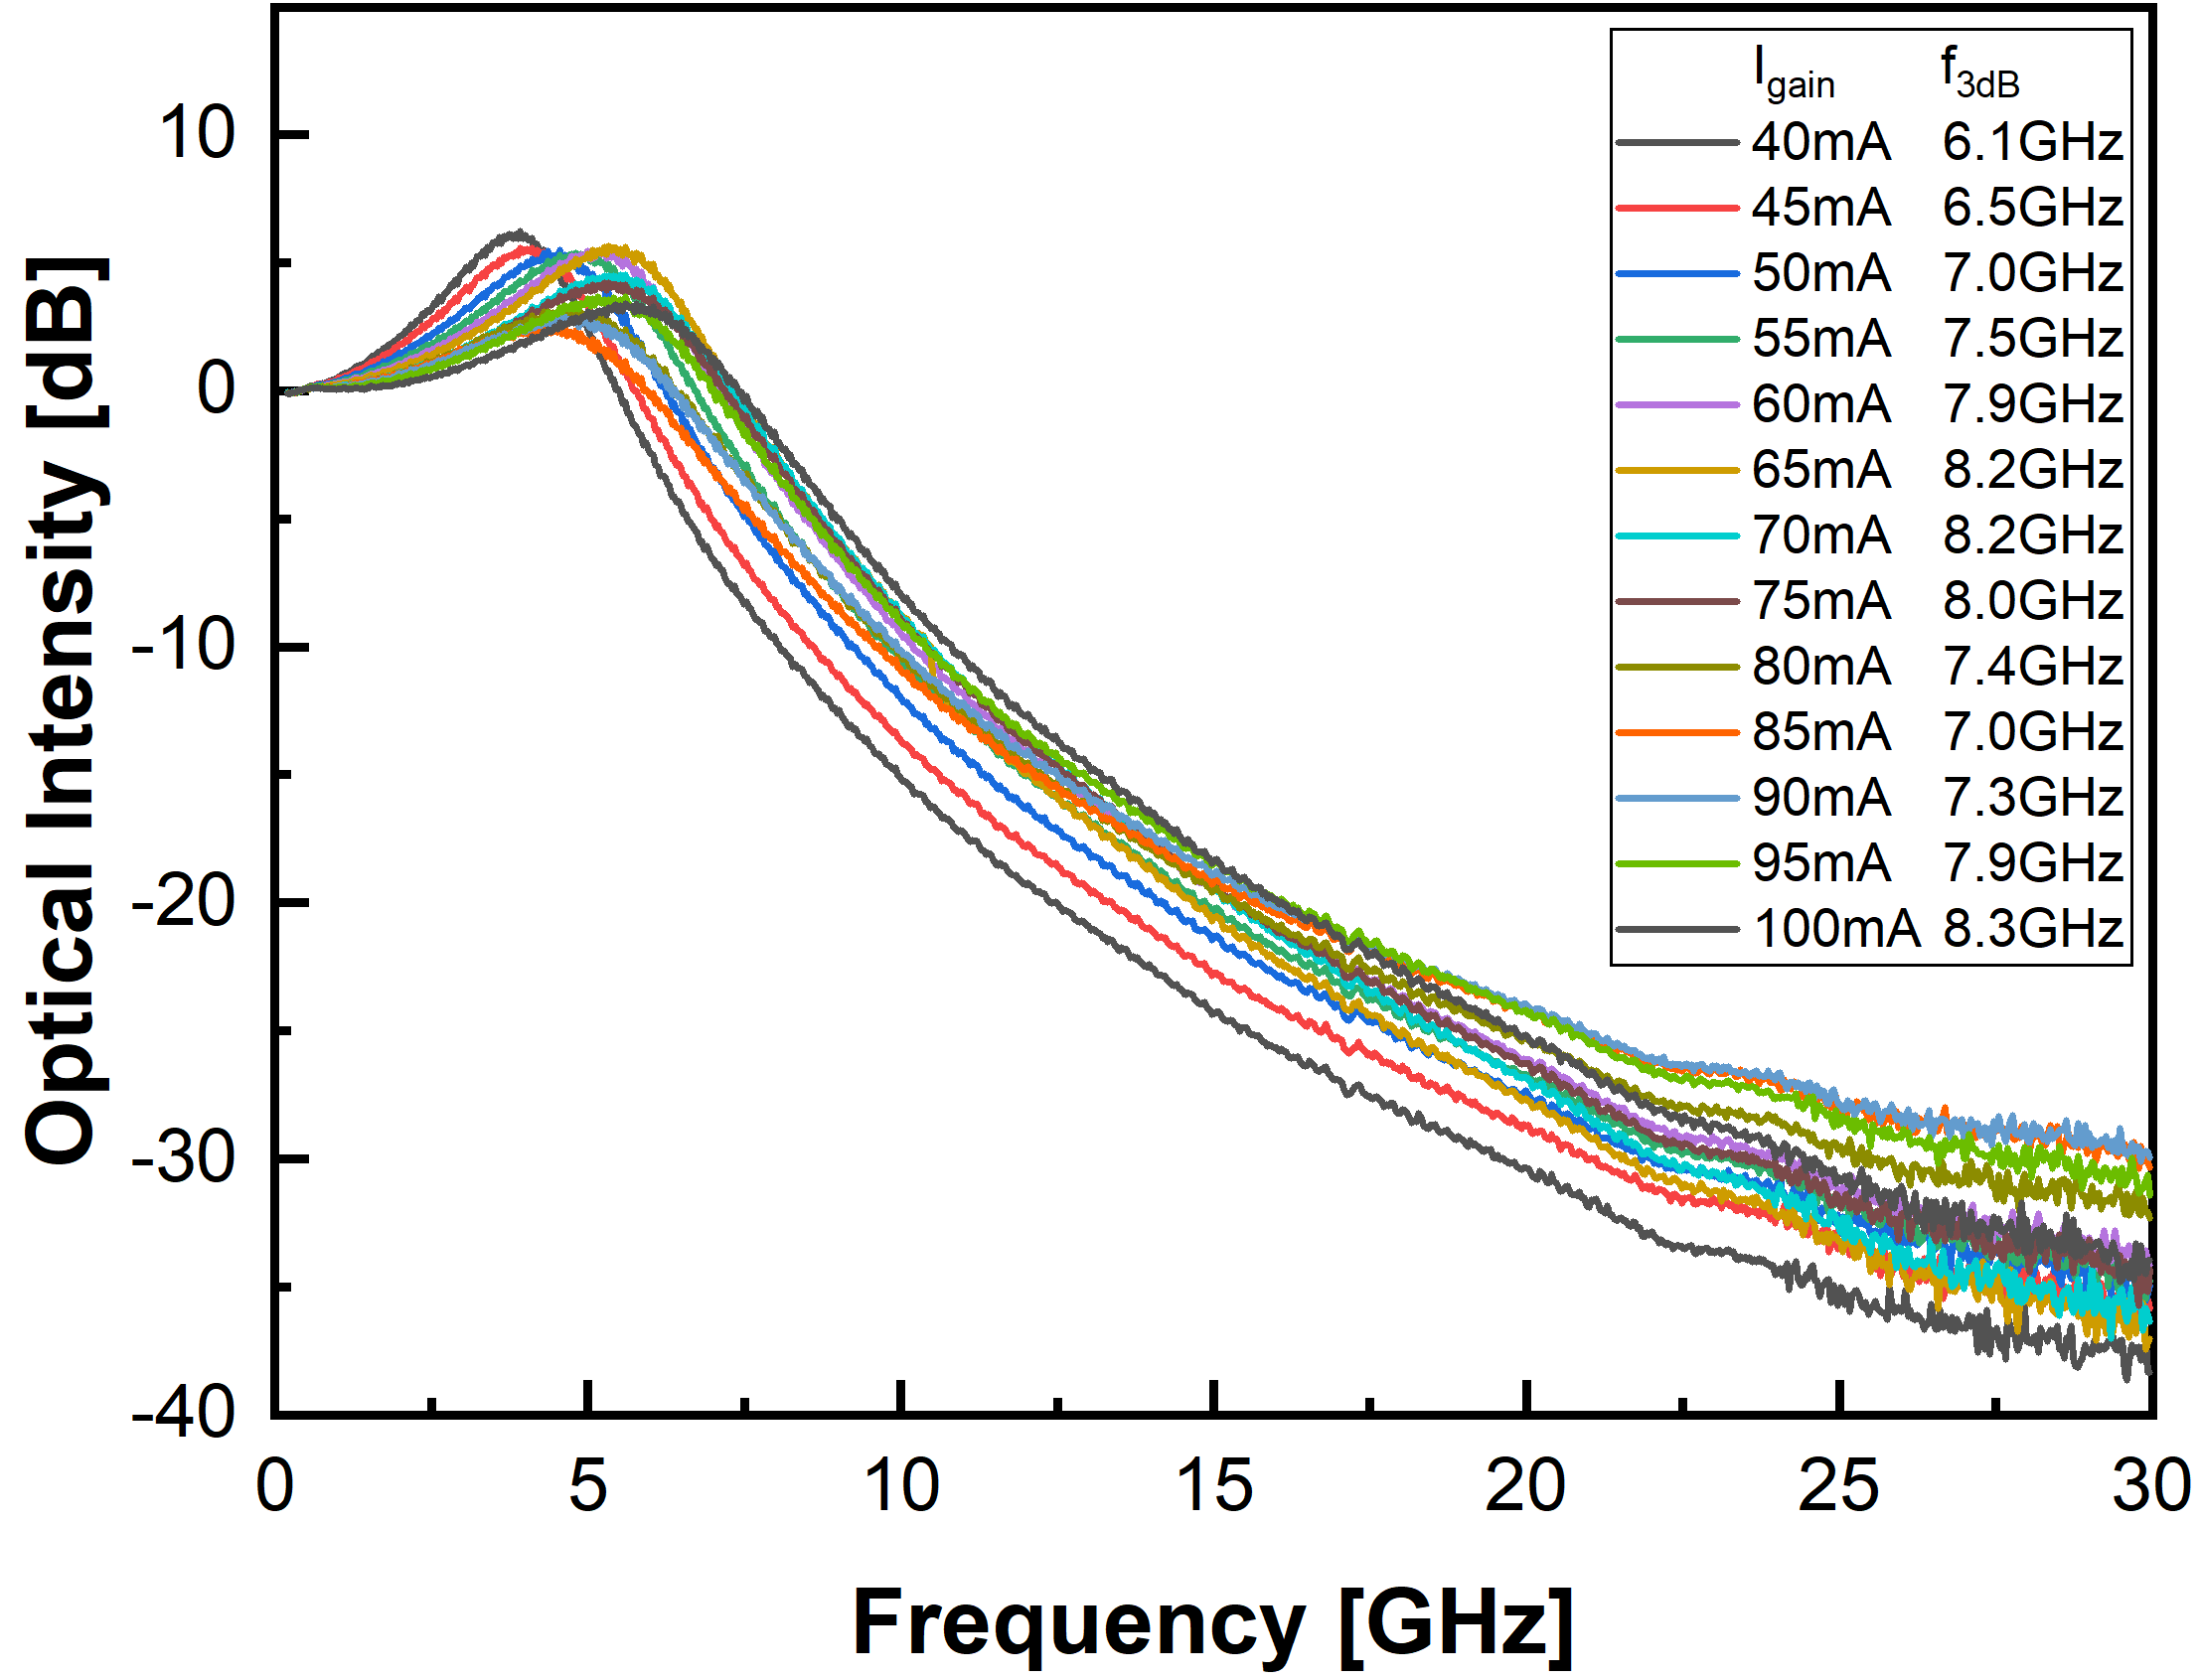
\includegraphics[width=0.7\linewidth]{figures/bandwidth_gain_scan_cleaved_4679.png}
%     \caption{Bandwidth measurements of a normal tunable DBR laser without feedback. The $f_{3dB}$ show a normal behavior that first increase with the applied gain current and then decrease}
%     \label{fig:bandwidth_gain_scan_cleaved_4679}
% \end{figure}

\begin{figure}[H]
    \centering
    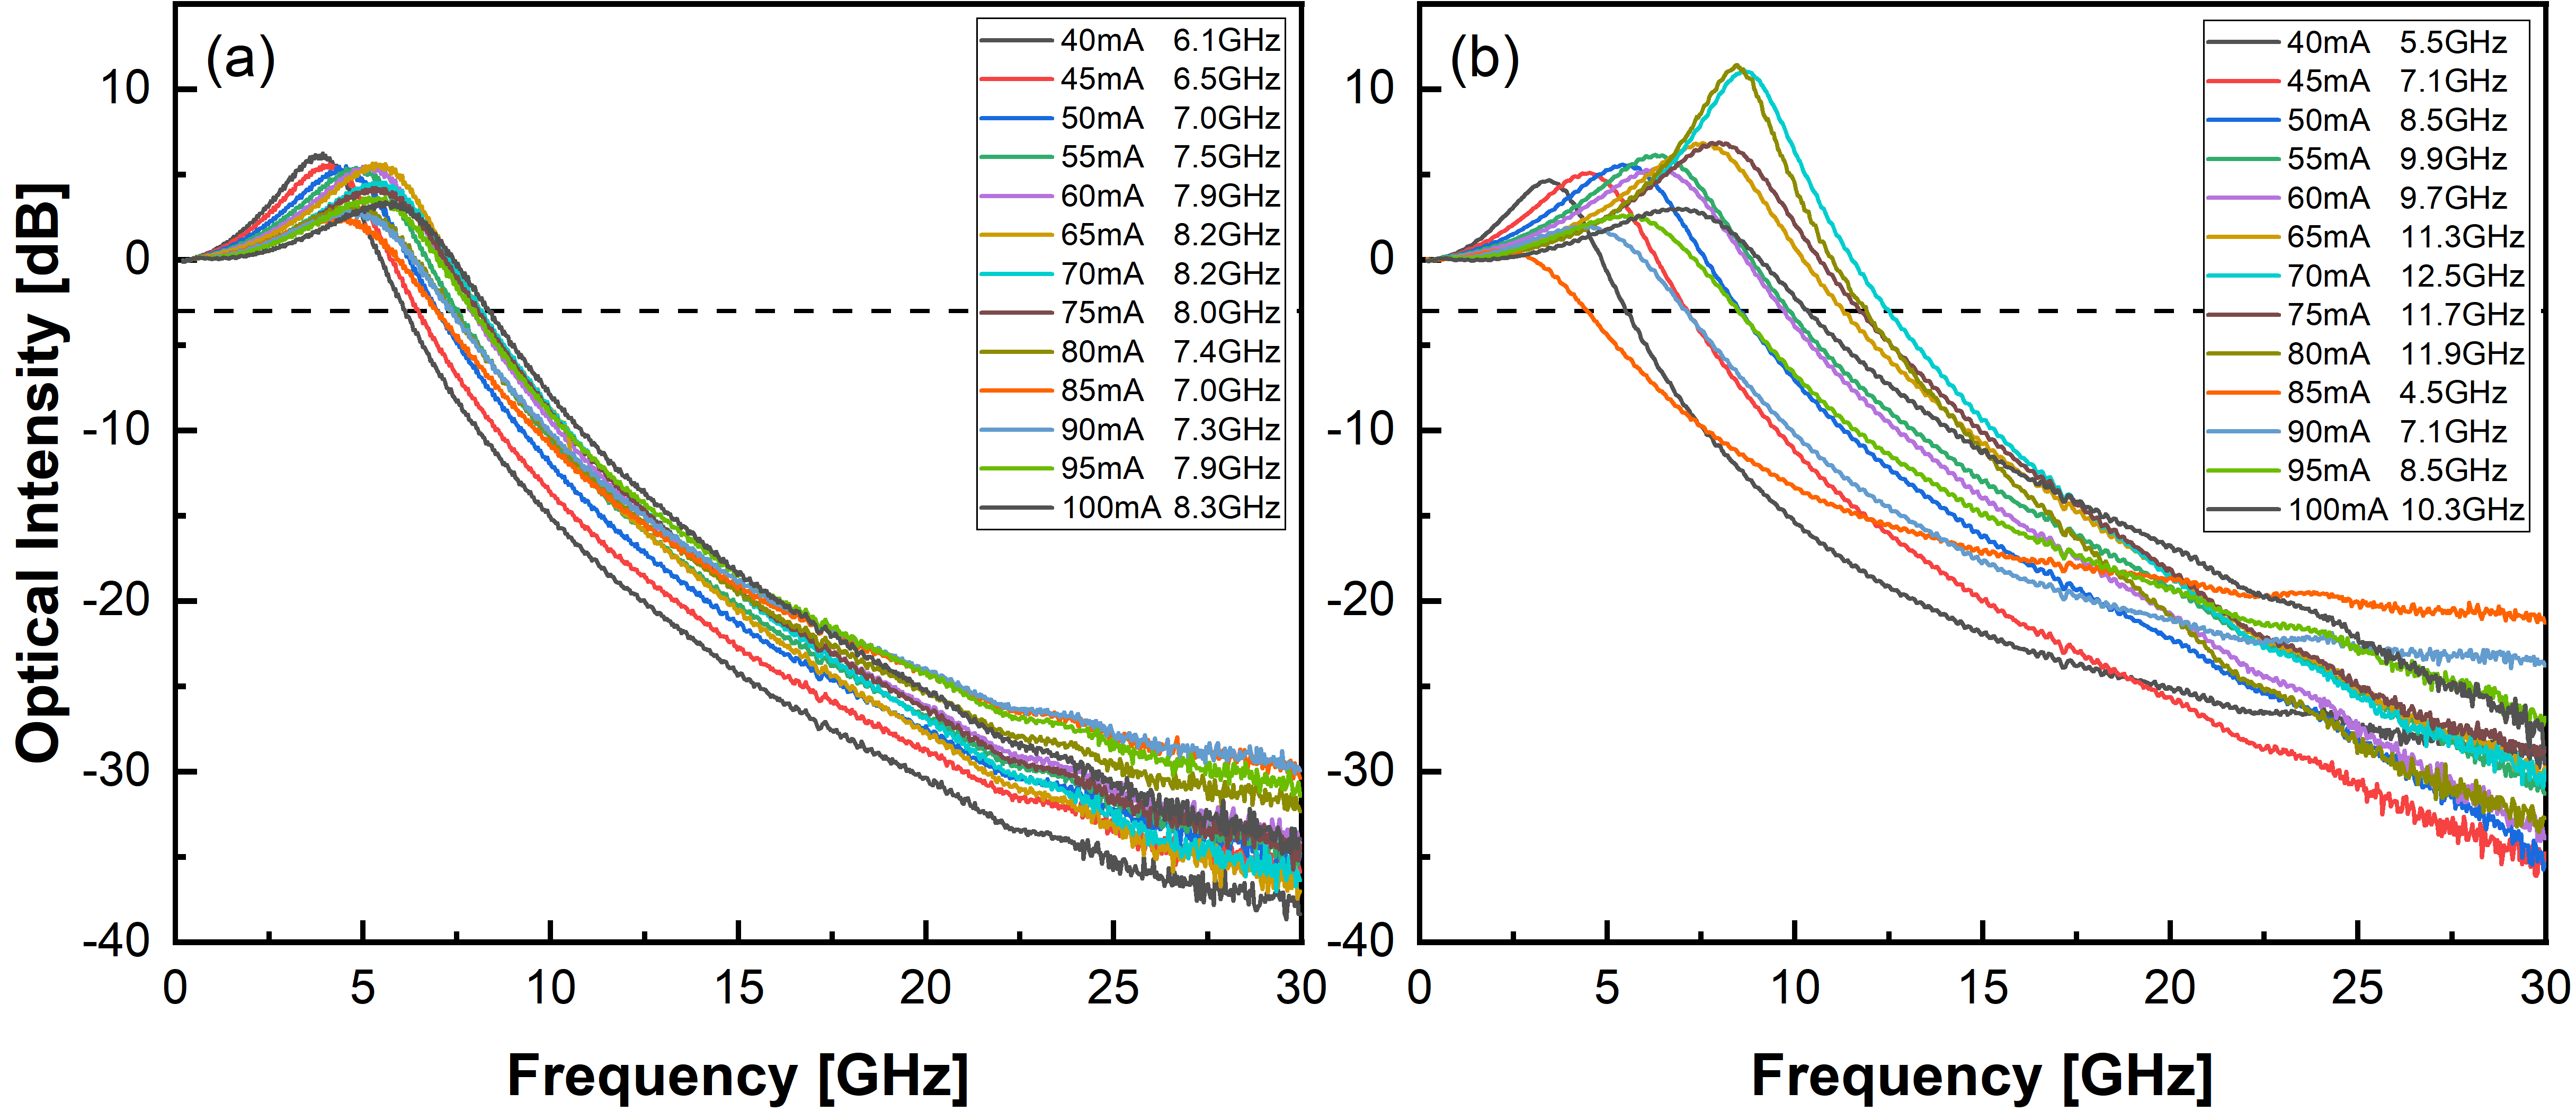
\includegraphics[width=\linewidth]{figures/bandwidth_gain_scan_cleaved_and_lensed_grating_4679.png}
    \caption{Bandwidth measurements of a polymer-based tunable DBR laser. (a) Without feedback, the $f_{3dB}$ shows a normal behavior that first increase with the applied gain current and then decrease, (b) with feedback, the prominant peaks at $65 \ mA$ and $70 \ mA$ permit the increased $f_{3dB}$ value compare with the laser without feedback.}
    \label{fig:bandwidth_gain_scan_cleaved_and_lensed}
\end{figure}

Without feedback, the increase of the relaxation oscillation freqeuncy $f_r$ along with rising of the gain current is observed and the intensity drop is due to the higher damping facor achieved at the higher gain current \cite{petermann2012laser}. The maximum bandwidth achieved is $8.2 \ GHz$ at $65 \ mA$ and $70\ mA$.

Compare to \autoref{fig:bandwidth_gain_scan_cleaved_and_lensed} (a), polymer-based tunable DBR laser operates differently with feedback, the intensity of the relaxation oscillation peak got enhanced especially at gain current $I_{gain}$ between $65 \ mA$ and $80 \ mA$, among these cases the maximum achieved bandwidth is $12.5 \ GHz$ at $70 \ mA$. The reason will be further discussed in \autoref{subsec:feedback_introduced_detuned_loading_measurement}.


% From a practical viewpoint the quantity of interest is the modulation bandwidth $\nu_B$ which indicates the frequency range over which the laser responds to the current modulation. It is usually defined as the frequency at which the modulation response has dropped by 3 dB relative to its low-frequency or DC value \cite{agrawal2013semiconductor}.
% \begin{figure}[ht]
%     \centering
%     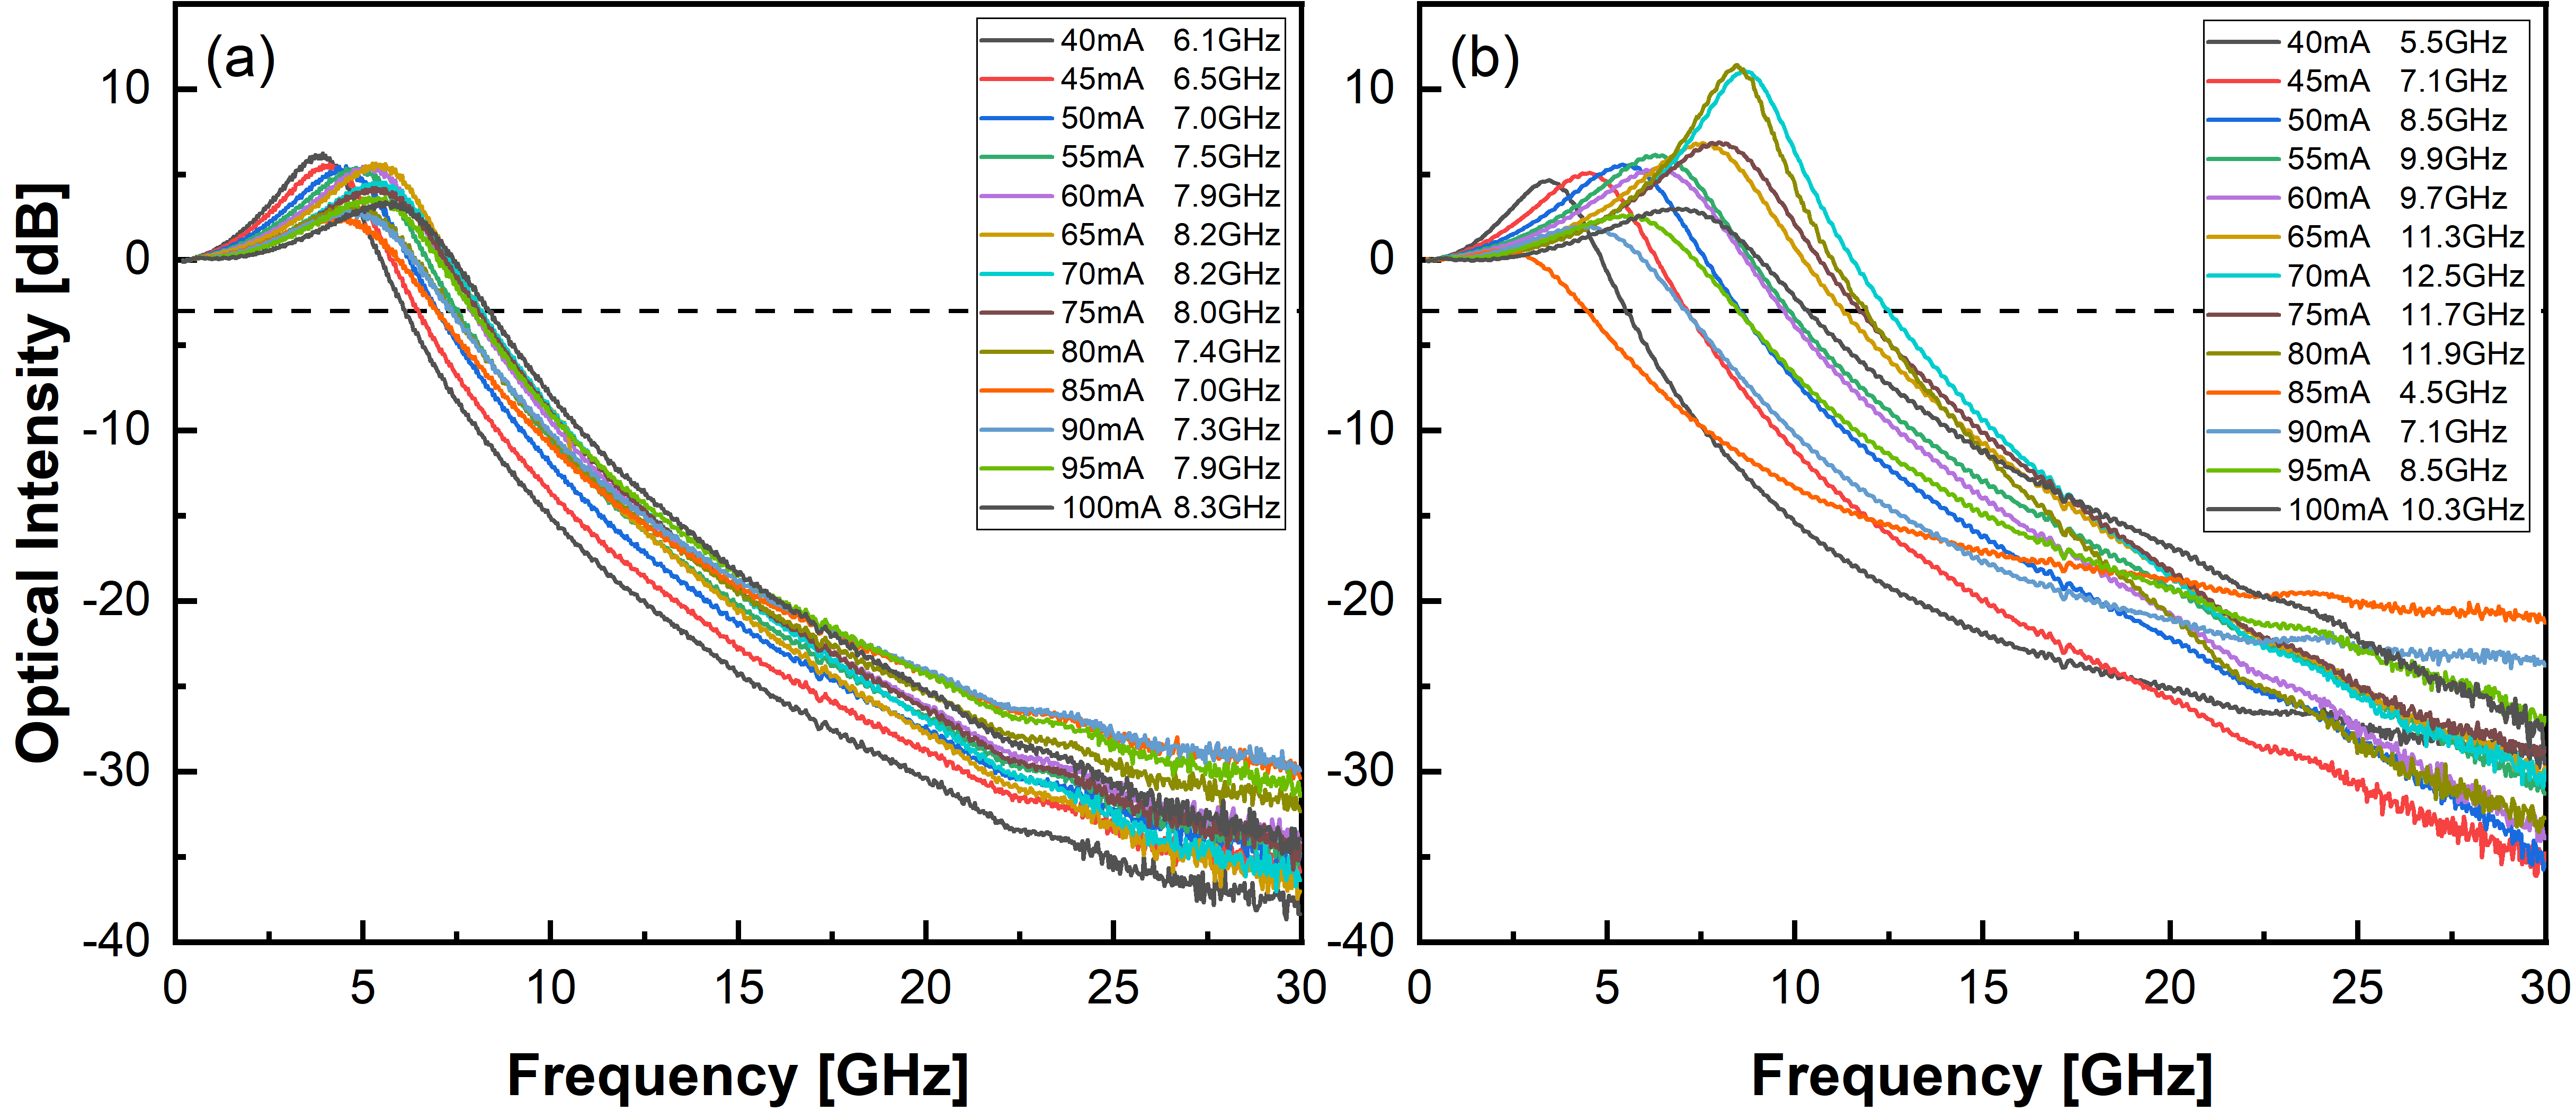
\includegraphics[width=\linewidth]{figures/bandwidth_gain_scan_cleaved_and_lensed_grating_4679.png}
%     \caption{Bandwidth measurements of a normal tunable DBR laser. (a) Without feedback, the $f_{3dB}$ show a normal behavior that first increase with the applied gain current and then decrease, (b) with feedback, the prominant peaks at 70 mA and 75 mA are due to the undamped RO peaks, at this condition, the $f_{3dB}$ got increased compare with the lase without feedback.}
%     \label{fig:bandwidth_gain_scan_cleaved_and_lensed}
% \end{figure}

% \begin{equation}
%     H(\omega)=\frac{\omega_R^2}{\omega_R^2-\omega^2-2j\omega\gamma}
%     \label{modulation_transfer_function}
% \end{equation}
% in \autoref{modulation_transfer_function}, $\omega_R$ is the relaxation resonance frequency and $\gamma$ is the damping factor.

% The relaxation oscillation frequency is a measure of the maximum modulation ability in semiconductor lasers through the injection current. Above the relaxation oscillation, the modulation efficiency is greatly degraded and intensity modulation through the injection current becomes difficult. [Semiconductor Lasers. Stability, Instability and Chaos.pdf]

\subsection{Detuend loading condition}\label{subsec:detuned_laoding_measurement}
In order to find the maximum achievable bandwidth for DBR laser without feedback, operating the tunable DBR laser under the detuned loading condition was measured and the result is shown in \autoref{fig:detuned_loading_measurement}. The measurement was performed by stabilizing the device at \SI{25}{\celsius} and using a gain current $I_{gain}=75 \ mA$. 

% which means the enhancement in \autoref{fig:bandwidth_gain_scan_cleaved_and_lensed} (b) is achieved not purely by detuned loading conditon without feedback effects.

\begin{figure}[ht]
    \centering
    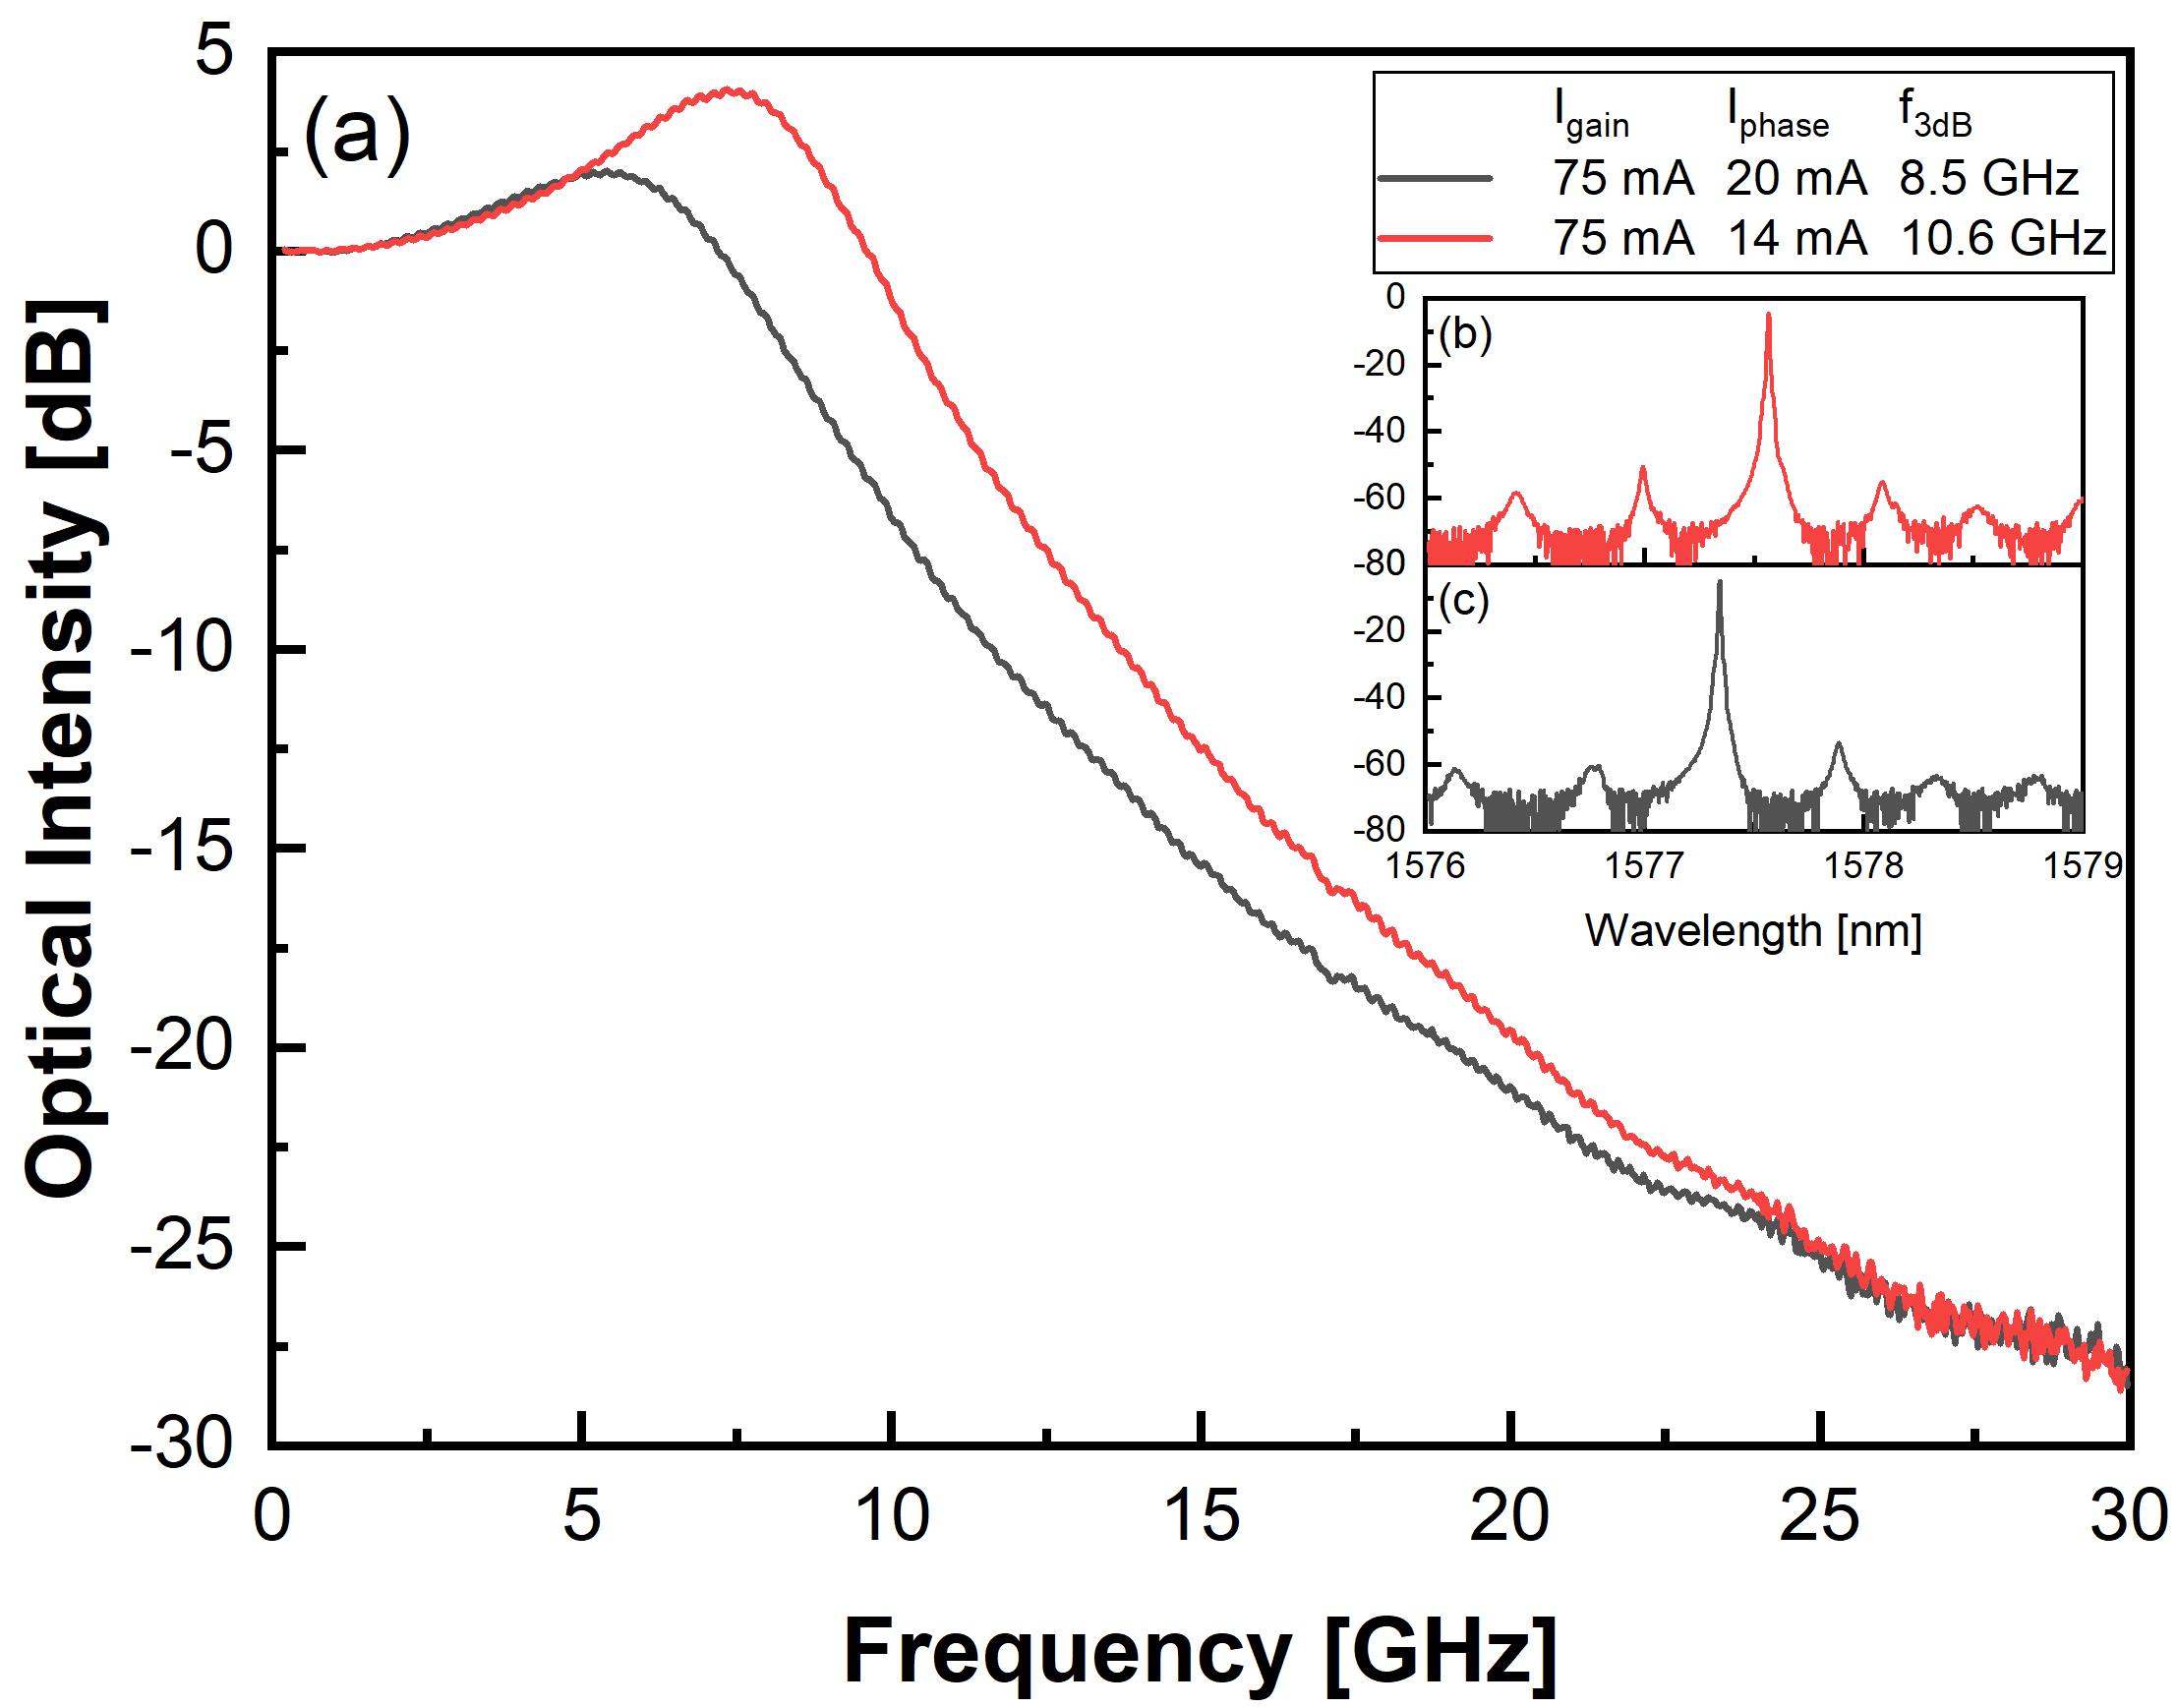
\includegraphics[width=\linewidth]{figures/detuned_loading.png}
    \caption{(a) Bandwidth enhancement with the detuned loading condition on DBR tunable laser. The red curve is detuned to the longer wavelength side of the grating response and it shows an increased bandwidth of 2.1 GHz compared to the grey curve without bandwidth enhancement effect, (b) spectrum when laser operates at longer wavelength side, (c) spectrum when laser operates at lower wavelength side.}
    \label{fig:detuned_loading_measurement}
\end{figure}

When the laser is lasing on the slope of the grating response, the side modes have a different gain spectrum relative to the peak of the grating response, which introduces the asymmetric behavior of the side modes as shown in \autoref{fig:detuned_loading_measurement} (b) and (c). In this case, when the left side mode is higher than the right one, means the lasing mode is operating at the longer wavelength side of the grating response, and vice versa. By increasing the phase current $I_{phase}$ from $14 \ mA$ to $20 \ mA$, the lasing mode is detuned from the longer wavelength side of the grating response to the shorter wavelength side. The maximum $f_{3dB}$ achieved at the longer wavelength side (red curve) is $10.6 \ GHz$ and the minimum (grey curve) is $8.5 \ GHz$. These two operating points also correspoinds to the red and grey points in \autoref{fig:detuned_loading_principle}.

\subsection{Feedback Introduced Detuned Loading}\label{subsec:feedback_introduced_detuned_loading_measurement}
As discussed in \autoref{sec:feedback_influenced_lasing_spectral_behavior}, the feedback from the output waveguide facet acts like a perturbation for the polymer-based tunable DBR laser which leads to self-modulation and undamped RO while shifting the phase. Combining this spectral behavior with the dutuned loading condition under feedback, further investigation was done using the same setting as in \autoref{subsec:detuned_laoding_measurement}, the result is shown in \autoref{fig:undamped_RO_measurement}.

\begin{figure}[ht]
    \centering
    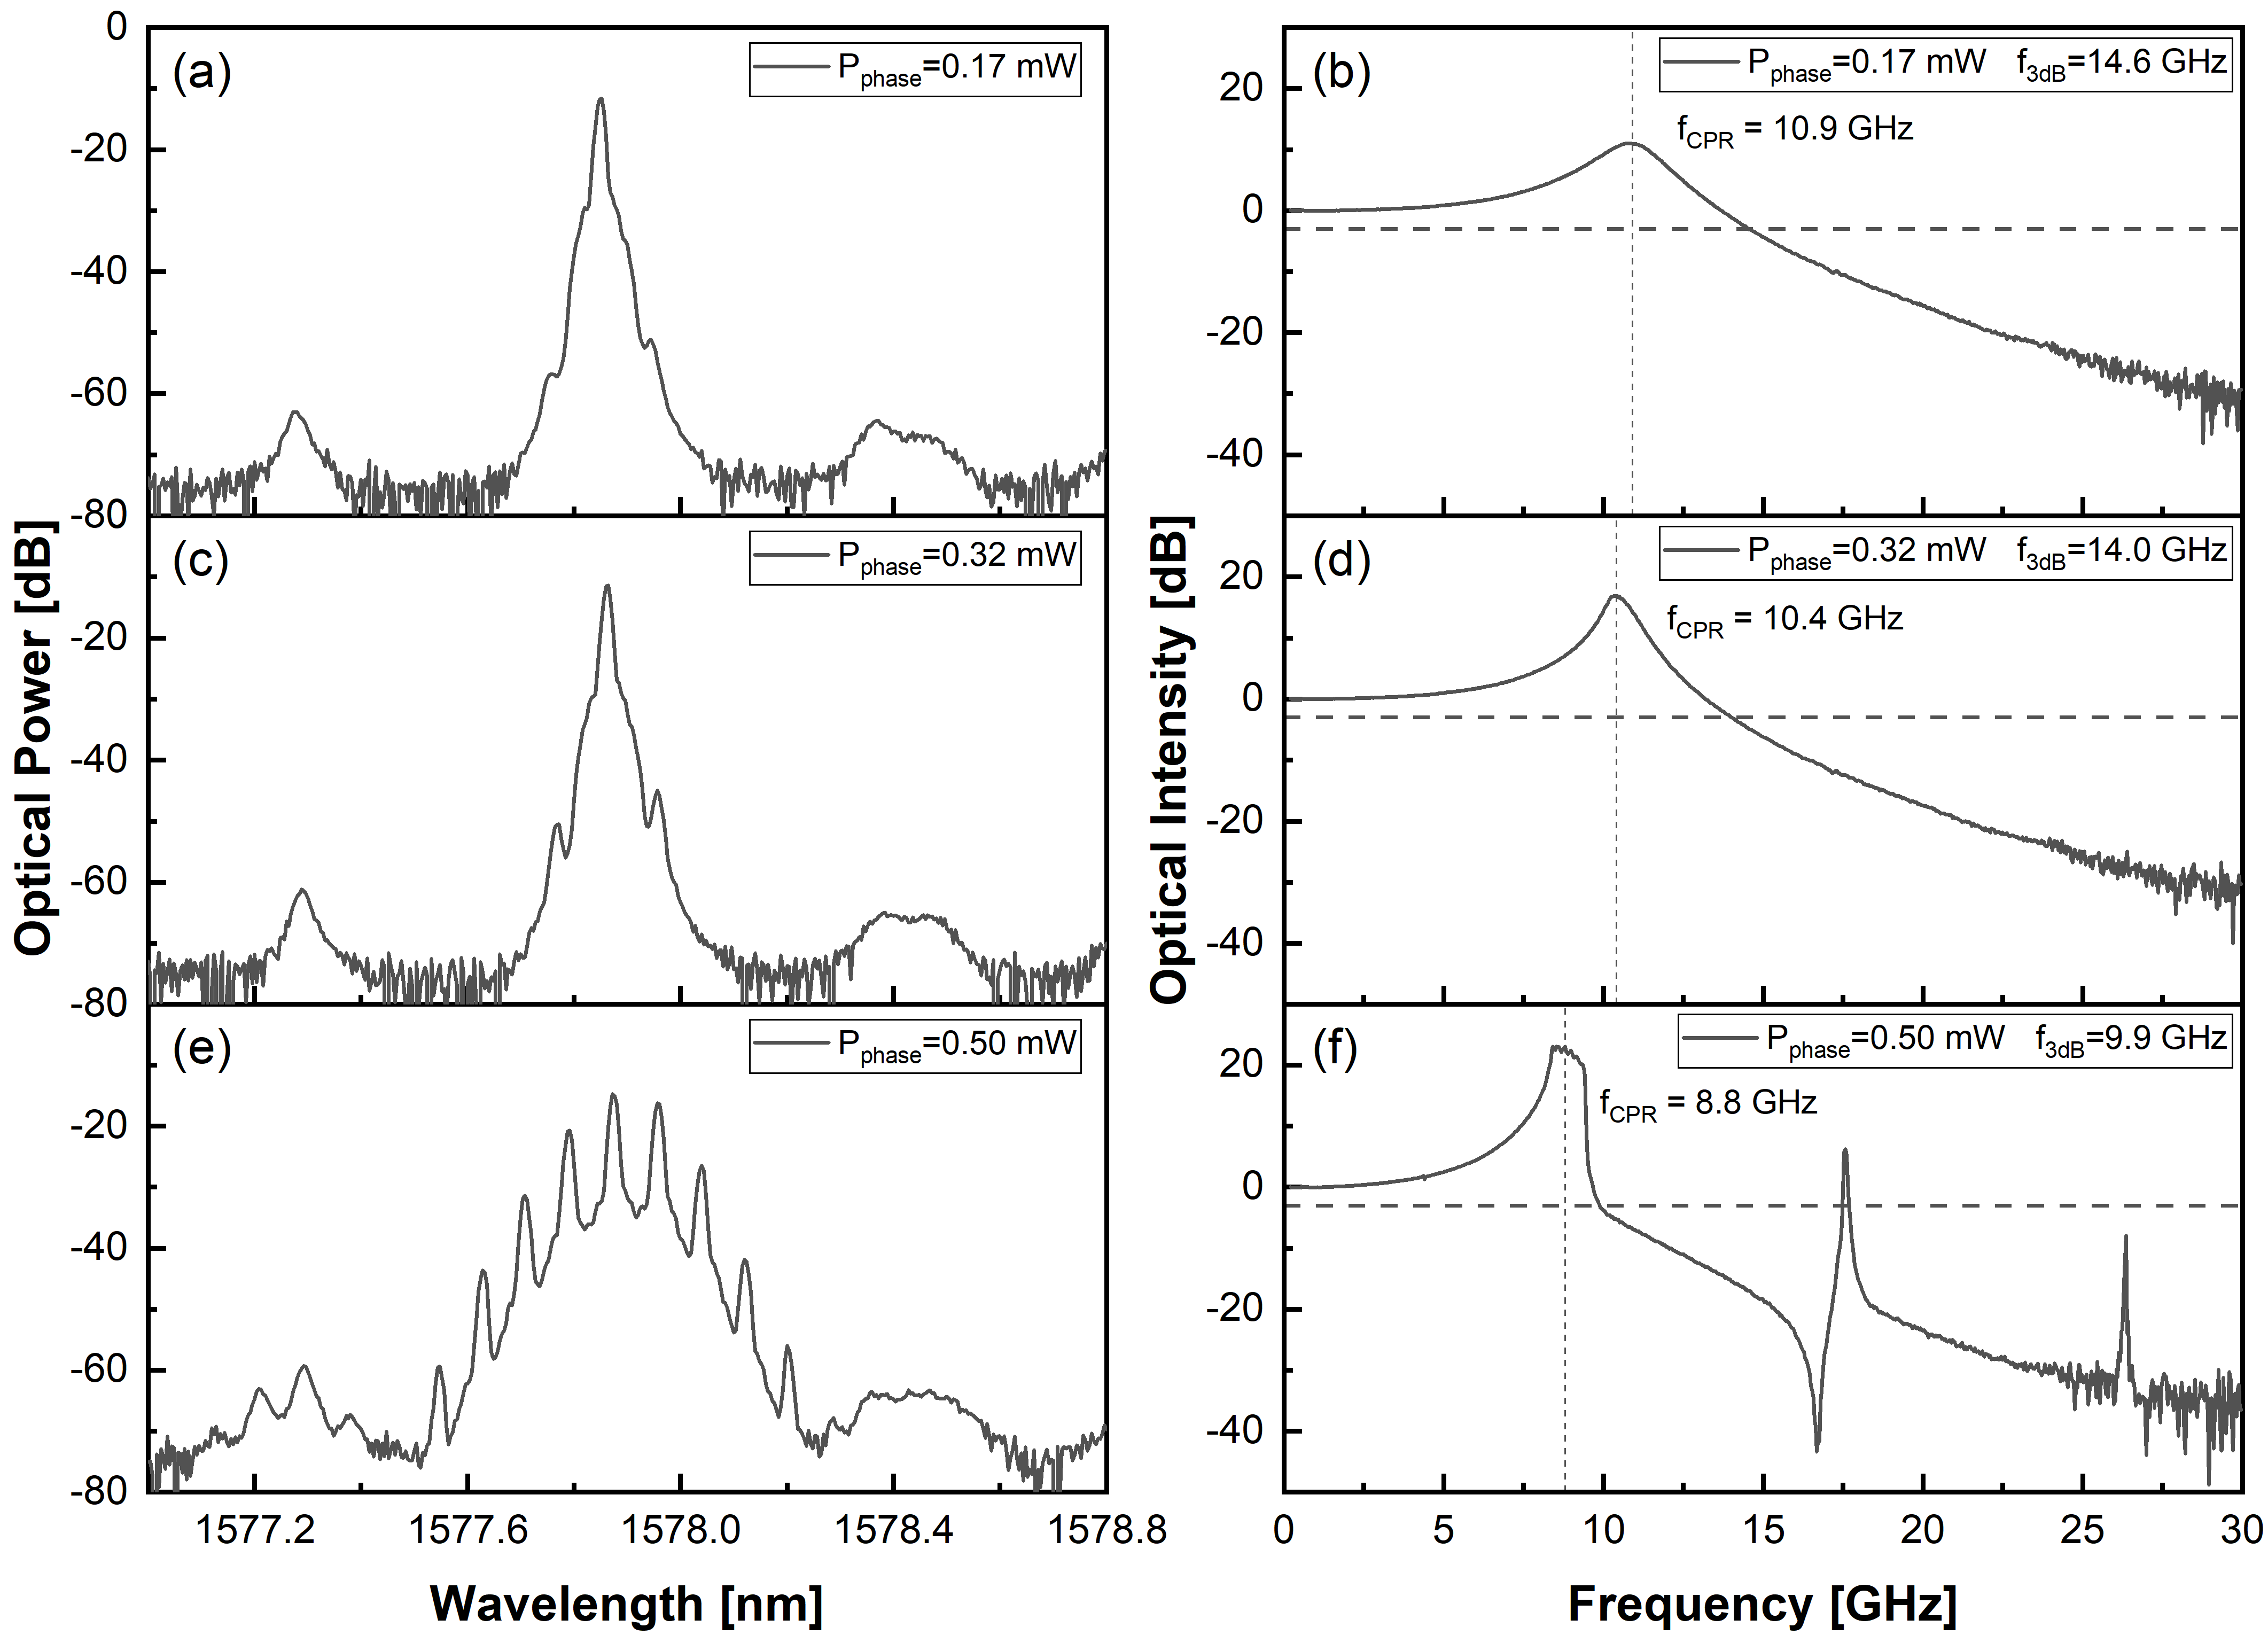
\includegraphics[width=\linewidth]{figures/Undamped_RO_and_bandwidth_grating_4621.png}
    \caption{Laser spectra and their corresponding intensity modulation curve. (a) Appearing of the undamped RO peak leads to a higher carrier-photon resonance in (b). (c) Growing of the side peaks leads to increase of the carrier-photon resonance peak in (d). (e) Drastic undamped RO leads to broadened lineshape and decreased modualiton bandwidth in (f).}
    \label{fig:undamped_RO_measurement}
\end{figure}
% \begin{figure}[ht]
%     \centering
%     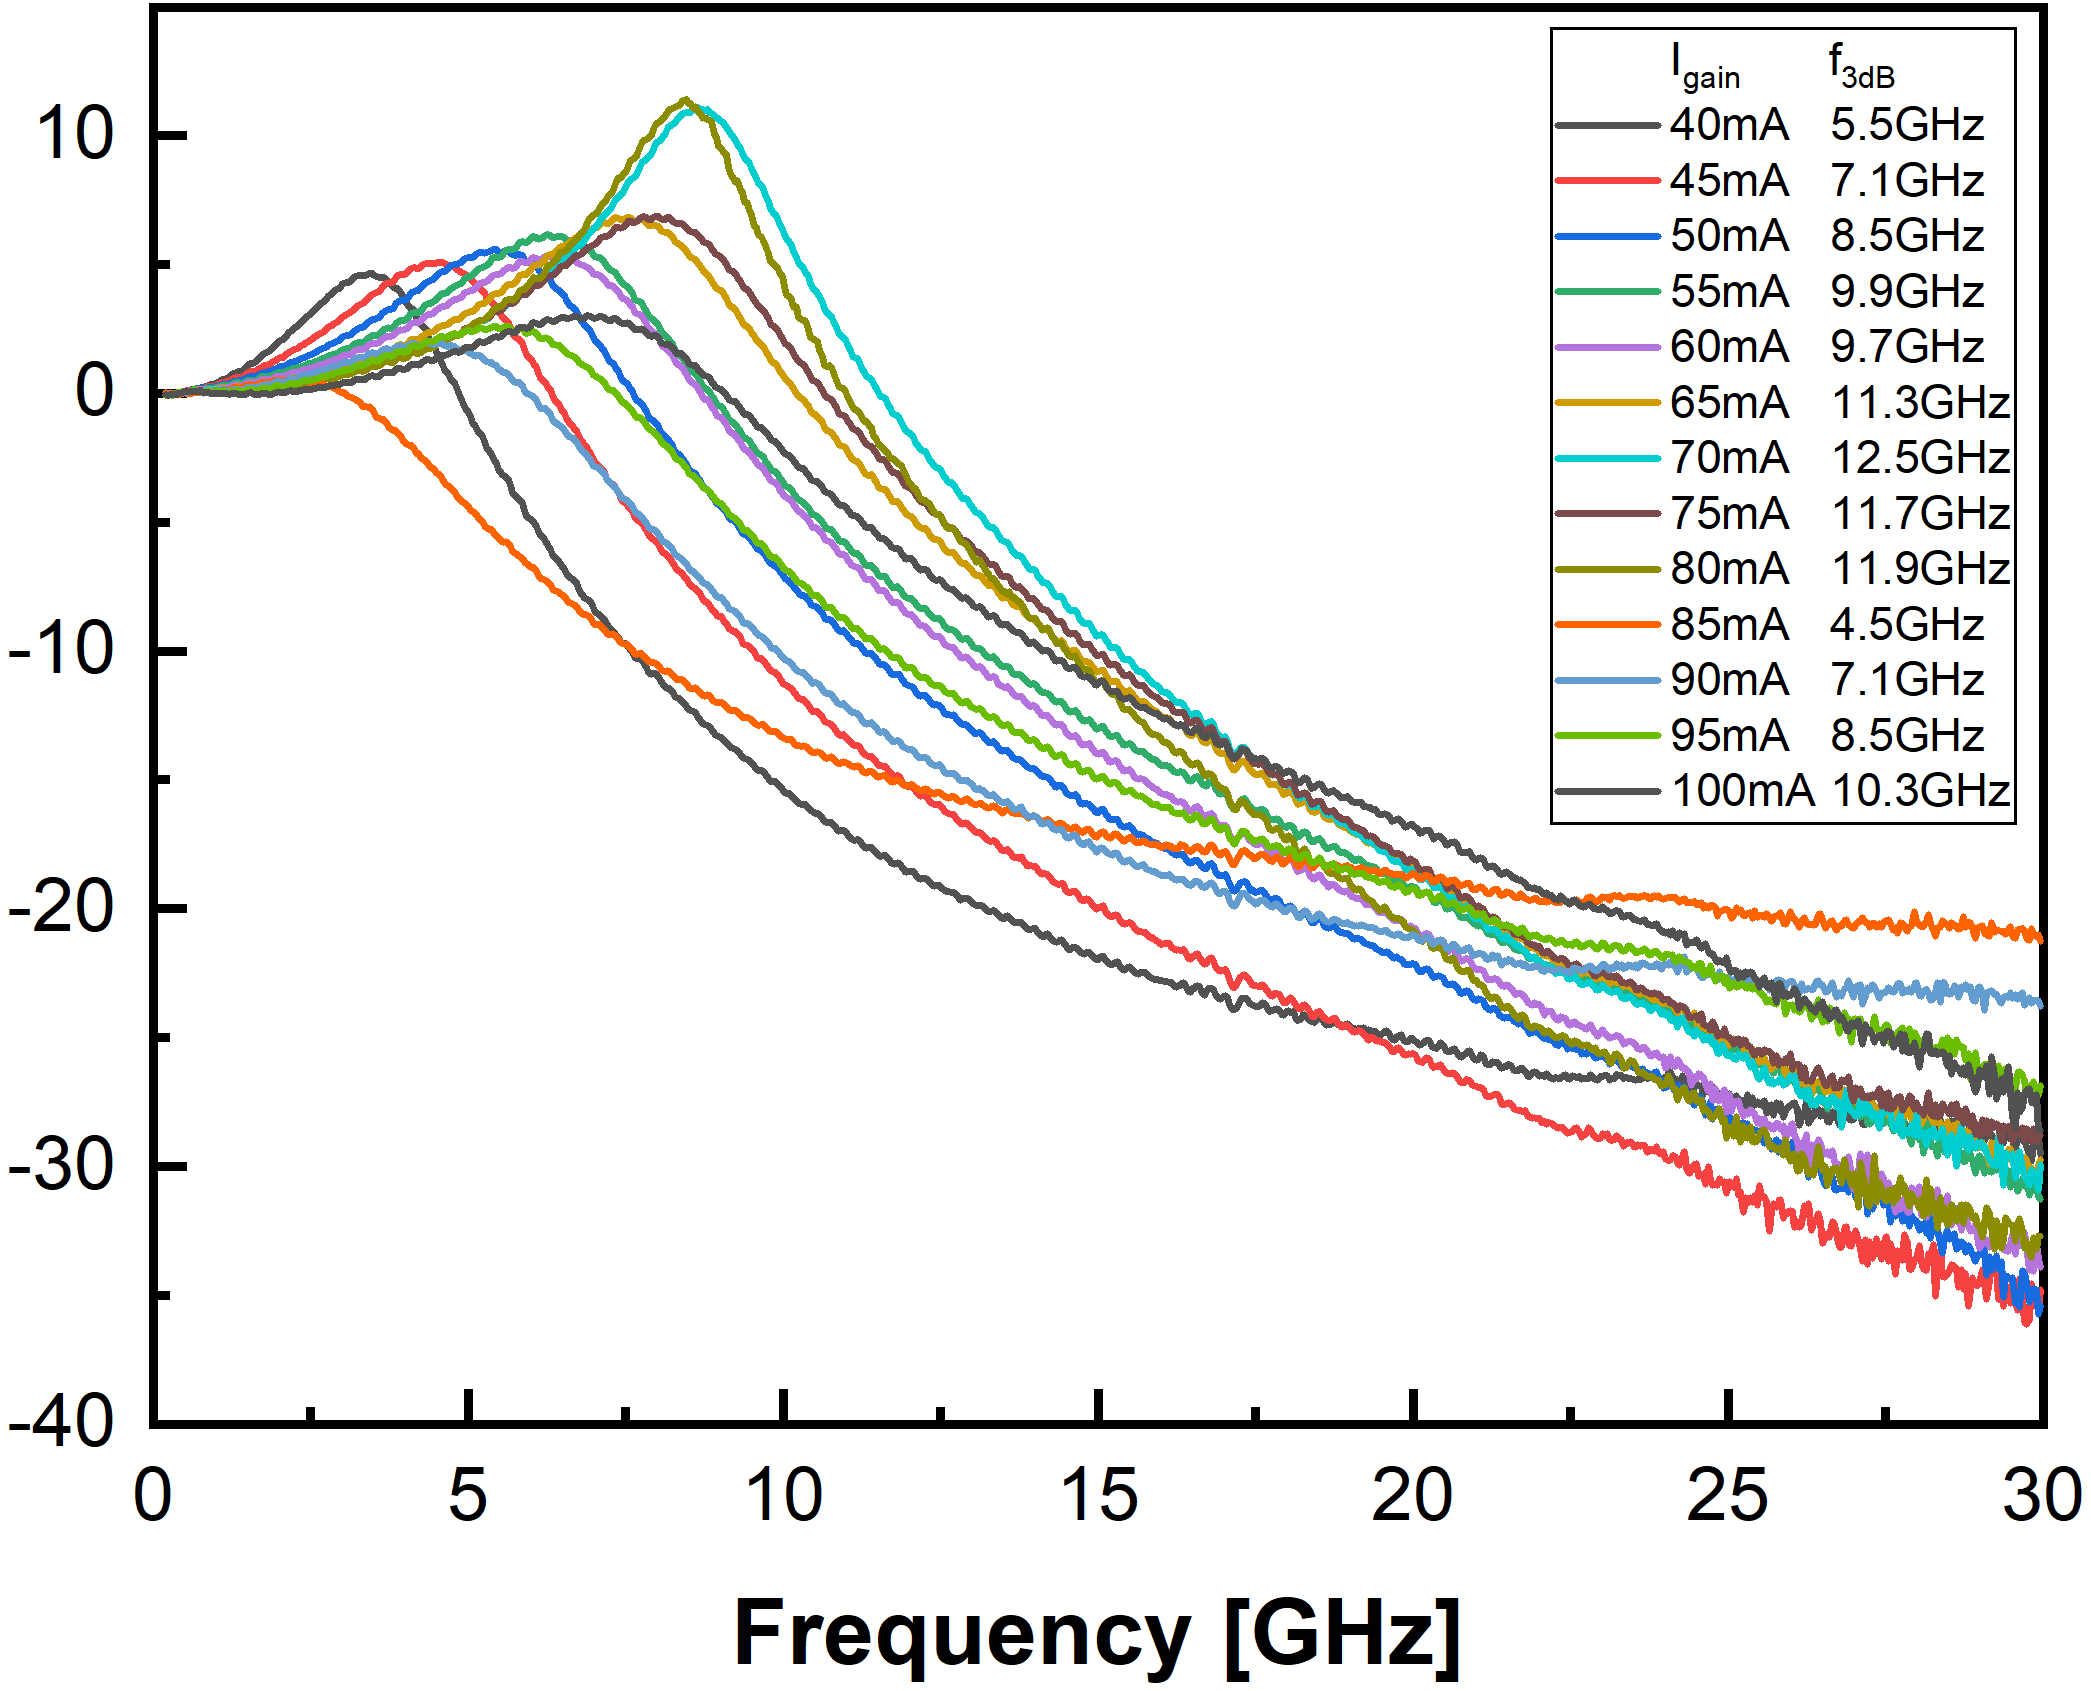
\includegraphics[width=0.7\linewidth]{figures/bandwidth_gain_scan_lensed_4679.png}
%     \caption{Bandwidth measurements of a normal tunable DBR laser with feedback, the prominant peaks at $65 \ mA$ and $70 \ mA$ are due to the self-modulation peaks, with the increased $f_{3dB}$ compare with the laser without feedback.}
%     \label{fig:bandwidth_gain_scan_lensed_4679}
% \end{figure}

The reason for the enhancement of the bandwidth can be seen from \autoref{fig:undamped_RO_measurement}. The appearing of the self-modulation side peaks leads to the carrier-photon resonance appears at a higher relaxation oscillation frequency which permits a higher $f_{3dB}$ value of $14.6 \ GHz$. Because of the phase tuning effect which relates to the dutuned loading condition, the side peaks slowly move towards the main peak with increasing intensity and the carrier-photon resonance become stronger with a slightly decreased relaxation oscillating frequency which leads to a $f_{3dB}$ value of $14.0 \ GHz$. As more side peaks appear in \autoref{fig:undamped_RO_measurement} (e), the strong undamped RO behavior leads to a broader lineshape and the intensity modulation shows prominent peaks with frequency corresponding to the mode spacing of the lasing side peaks. This last behavior in \autoref{fig:undamped_RO_measurement} (e) leads to broadened lineshape and significantly decreases the $f_{3dB}$ compare to the other two cases. The increase of the relaxation oscillation intensity and the enhancement of bandwidth shown in \autoref{fig:bandwidth_gain_scan_cleaved_and_lensed} (b) is certainly related to the occurence of the side peaks as shown in \autoref{fig:undamped_RO_measurement} (a)-(d). The maximum achieved bandwidth $f_{3dB}$ is $14.6 \ GHz$ for polymer-based tunable DBR laser with feedback. Photon-photon resonance was not observed in this case.

% \subsection{}
% \textit{Chirp arises because the frequency of the laser mode depends on the carrier number in the active region. Above threshold, the carrier number changes because of two effects: spectral hole burning prohibits the perfect pinning of the carrier number and permits adiabatic chirp, and during transients, there are relaxation oscillations of carrier number, which cause dynamic chirp. [Kazarinov 1987]}

% \textit{Current modulation of the active region results in a modulation of both the photon density and the carrier density. The modulation of the carrier density modulates the gain; however, it also modulates the index of the active region na . As a result, the optical length of the cavity is modulated by the current, causing the resonant mode to shift back and forth in frequency. [Larry A. Coldren.pdf]}

% If we consider the case discussed earlier where the semiconductor cavity is extended by a passive section of length $L_1$, with a nonreflective transition between the two sections, the reflection at the semiconductor section constant in magnitude, but has a frequency-dependent phase shift with $d\phi_r/d\omega = 2L_1/v_g1$ where $2L/v_g1$ is the roundtrip time in the external cavity. Therefore, in this case $B=0$, the chirp reduction factor is [Kazarinov 1987]



\section{Chirp Parameter ($\alpha$-factor) Measurement}\label{sec:chirp_measurement}
Since the linewidth enhancement factor $\alpha$ is highly dependent on the spectral detuning \cite{soriano2013complex}, two measurement methods are performed to get the right characterization for DBR laser with feedback.

\subsection{Measurement with Lightwave Component Analyzer}\label{subsec:measurement_with_LCA}
First method by using the Lightwave Component Analyzer (LCA) of \autoref{fig:LCA_setup} measures the small signal frequency response of a light emitter, a dispersive medium and a light receiver. The dispersive medium is a standard single mode fiber of $81 \ km$ and an Er-doped fiber amplifier pumped at 1.55 $\mu m$. Resonance frequencies are observed as sharp peaks in the frequency response.
\begin{figure}[ht]
    \centering
    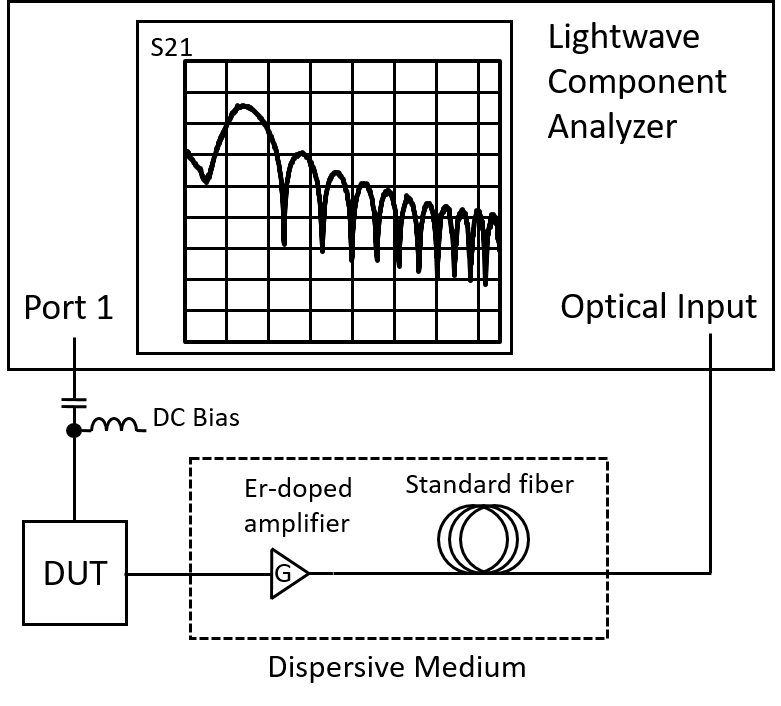
\includegraphics[width=.5\linewidth]{figures/LCA_setup.png}
    \caption{Schematic set-up for chirp parameter measurement using Lightwave Component Analyzer.}
    \label{fig:LCA_setup}
\end{figure}

The measurement principle can be explained as following, the output optical intensity is assumed as \cite{devaux1993simple}
\begin{equation}
    I=I_0(1+mcos(2\pi ft)) \qquad with \ m \ll 1
    \label{eq:chirp_optical_intensity}
\end{equation}
with $m$ being the modulation depth and $f$ the modulation frequency of light intensity. The frequency response which is measured by the set-up described above is then \cite{devaux1993simple}
\begin{equation}
    I_f=I_0m\sqrt{1+\alpha^2}\abs{\cos\qty(\frac{\pi\lambda^2DLf^2}{c}+\arctan(\alpha))}.
    \label{eq:chirp_optical_frequency}
\end{equation}

The resonance frequencies $f_u$ (as shown in \autoref{fig:chirp_cleaved_and_lensed} (a), (c)) correspond to the $u^{th}$-zeros of \autoref{eq:chirp_optical_frequency}. They follow the following equation \cite{devaux1993simple}
\begin{equation}
    f_u^2L=\frac{c}{2D\lambda ^2}\qty(1+2u-\frac{2}{\pi}arctan(\alpha))
    \label{eq:LCA_equation}
\end{equation}
which is the result of two simultaneous interferences between the carrier and the two sidebands. Plotting $f_u^2L$ versus $2u$ gives a straight line whose slope and position yield the dispersion and the chirp parameter by linear regression. The frequency of the first dip is determined primarily by $\alpha$, and to a lesser extent by $D$, whereas the frequency of the second dip is determined primarily by $D$ and to a lesser extent by $\alpha$, $D$ is the fiber dispersion coefficient \cite{srinivasan1995using}.

The frequency response form LCA and fitted linear regression data are shown in \autoref{fig:chirp_cleaved_and_lensed}, the obtained $\alpha$ parameter in two conditions is compared in \autoref{tab:chirp_alpha_comparison}. The deviated $\alpha$ parameter at $80 \ mA$ with a value of 4.13 can be clearly seen from \autoref{fig:chirp_cleaved_and_lensed} (c), whereas the position of the first dip of the purple curve which indicates $80 \ mA$ is devaited from the other current values, it may come from the effect of undmaped RO since in \autoref{fig:bandwidth_gain_scan_cleaved_and_lensed} (b) at $80 \ mA$ the self-modulation introduced increase of relaxation oscillation peak appears. Except for this current value, the achieved $\alpha$ parmaerters with feedback are generally lower than the without feedback case. The different calculated $F$ factor may come from shifting of the phase by increasing the current value.

\begin{figure}[H]
    \centering
    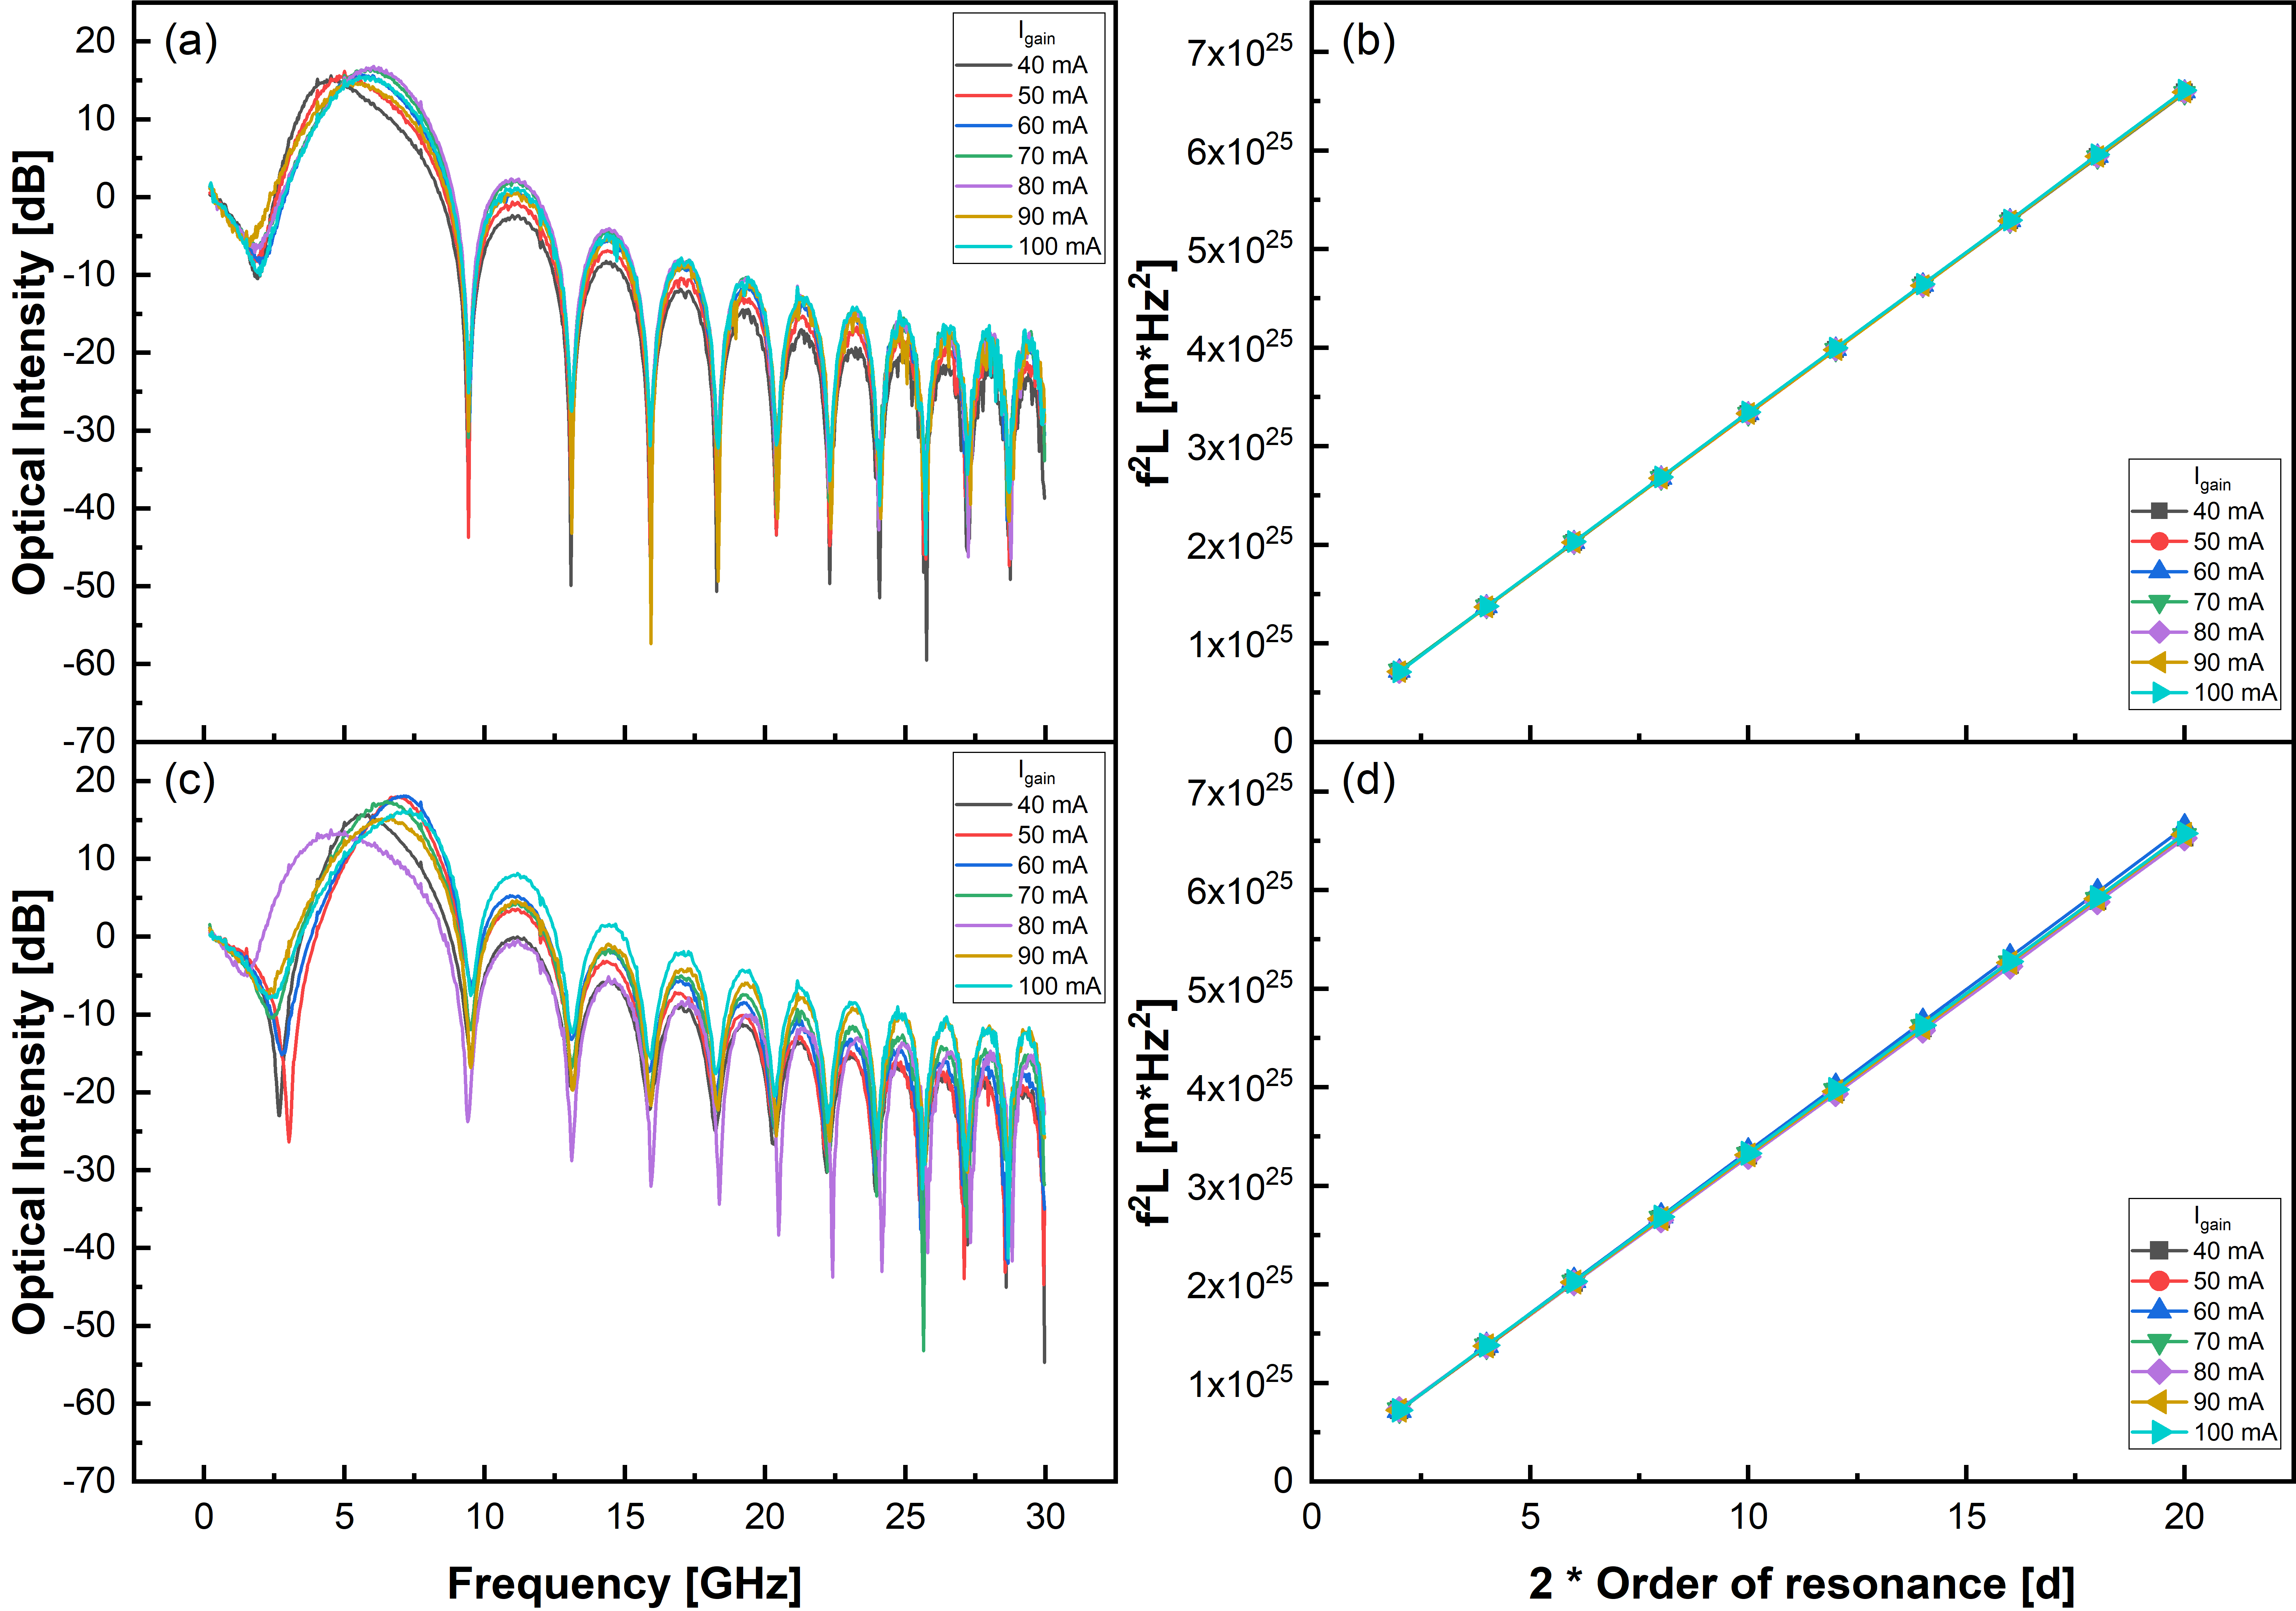
\includegraphics[width=\linewidth]{figures/chirp_cleaved_and_lensed_4679.png}
    \caption{Frequency response from the LCA measurement, (a) without feedback, (c) with feedback. Resonance frequencies squared (x-axis of (a) and (c)) times fiber length ($81 \ km$) versus two times the order of the resonance, (b) without feedback, (d) with feedback. Linear regression allows to find the chirp parameter and the dispersion from \autoref{eq:LCA_equation}.}
    \label{fig:chirp_cleaved_and_lensed}
\end{figure}

\begin{table}[ht]
    \centering
    \caption{Comparison of achieved $\alpha$ parameter value. Laser with feedback in general shows a decreased $\alpha$ value at all current values except for $80 \ mA$. The different calculated $F$ factor may come from shifting of the phase by increasing the current value.}
    \label{tab:chirp_alpha_comparison}
    \begin{tabular}{@{}llll@{}}
    \toprule
    \multirow{2}{*}{Current {[}mA{]}} & \multicolumn{2}{c}{$\alpha$} & \multicolumn{1}{c}{$F$} \\
                                      & w/o feedback   & w/feedback  & Chirp reduction factor  \\ \midrule
    40                                & 3.904          & 2.768       & \multicolumn{1}{c}{1.410}                   \\
    50                                & 3.771          & 2.383       & \multicolumn{1}{c}{1.582}                   \\
    60                                & 3.336          & 2.658       & \multicolumn{1}{c}{1.255}                   \\
    70                                & 3.837          & 2.998       & \multicolumn{1}{c}{1.280}                   \\
    80                                & 3.756          & 4.13        & \multicolumn{1}{c}{0.909}                   \\
    90                                & 3.97           & 2.934       & \multicolumn{1}{c}{1.353}                   \\
    100                               & 3.299          & 2.912       & \multicolumn{1}{c}{1.133}                   \\ \bottomrule
    \end{tabular}
\end{table}

\subsection{AM-FM Index Method}
The $\alpha$ parameter can also be obtained from measurements of the optical intensity spectrum. For this measurement technique, the ratio of residual phase modulation to amplitude modulation is measured from the optical spectrum of the laser when it is modulated with a sinusoidal signal of frequency $f$, the output optical intensity is assumed same as \autoref{eq:chirp_optical_intensity}. The optical intensiy spectrum of this signal is characterized by and optical carrier with power $I_0$, and two first oder sidebans with average power given by \cite{harder1983measurement}
\begin{equation}
    \overline{I_{\pm 1}}=I_0\qty(\frac{m}{4})^2\qty(1+\qty(\frac{2p}{m})^2) \qquad with \ m \ll 1
\end{equation}
where $p$ is the phase modulation index \cite{harder1983measurement}, which is related to the chirp parameter by \cite{bjerkan1996measurement}
\begin{equation}
    \frac{2p}{m}=\alpha\sqrt{1+\qty(\frac{f_c}{f})^2}
    \label{eq:chirp_alpha}
\end{equation}
where $f_c$ is the chirp frequency. For modulation frequencies $f \gg f_c$, \autoref{eq:chirp_alpha} results to \cite{harder1983measurement}
\begin{equation}
    \frac{2p}{m}=\alpha
    \label{eq:chirp_alpha_2}
\end{equation}
By measuring the power in the carrier and the sidebands from the optical spectrum, the paratmeter $p$ can be obtained. The value of $m$ can be obtained from the instanteneous power signal, therefore $\alpha$ parameter is characterized \cite{villafranca2007precise, harder1983measurement}.

The $\alpha$ parameter measurement results are shown in \autoref{fig:Alpha_Cleaved_and_Lensed}. For laser with feedback the $\alpha$ parameter value ranges from $-4.581$ to $-1.208$ where as for laser without feedback it is from $-4.944$ to $-2.36$. Lower $\alpha$ value of $-1.208$ is achieved for laser with feedback. It shows a similar result as the method in \autoref{subsec:measurement_with_LCA} and the $\alpha$ parameter under feedback conditions is decreased can be confirmed.
% The experimental arrangement for measuring the intensity and phase modulation index is shown in Fig. 1. The semiconductor laser is biased above threshold and a small sinusoidally varying current at frequency $\Omega$ is superimposed. The intensity and spectral density of the radiation field are given by [Harder, Vahala et al 1983]
% \begin{equation}
%     Intensity: E_0^2[1+mcos(\Omega t)]
% \end{equation}
% \begin{equation}
%     Spectrum: Center \ line \ at \ \omega_1: E_0^2[J_0^2(\beta)+m^2J_1^2(\beta)]
%     \label{eq:alpha_2}
% \end{equation}
% \begin{equation}
%     First \ sidebands \ at \
%     \ \omega_1 \pm \Omega: E_0^2\big\{J_1^2(\beta)+1[(m/2)(J_2(\beta)-J_0(\beta))]^2\big\}
%     \label{eq:alpha_3}
% \end{equation}
% The phase modulation index $\beta$ can be found by measuring the relative sideband strength and using \autoref{eq:alpha_2} and \autoref{eq:alpha_3}. The factor $\alpha_m$ is then obtained as $\alpha_m = -2(\beta/m)$.
\begin{figure}[ht]
    \centering
    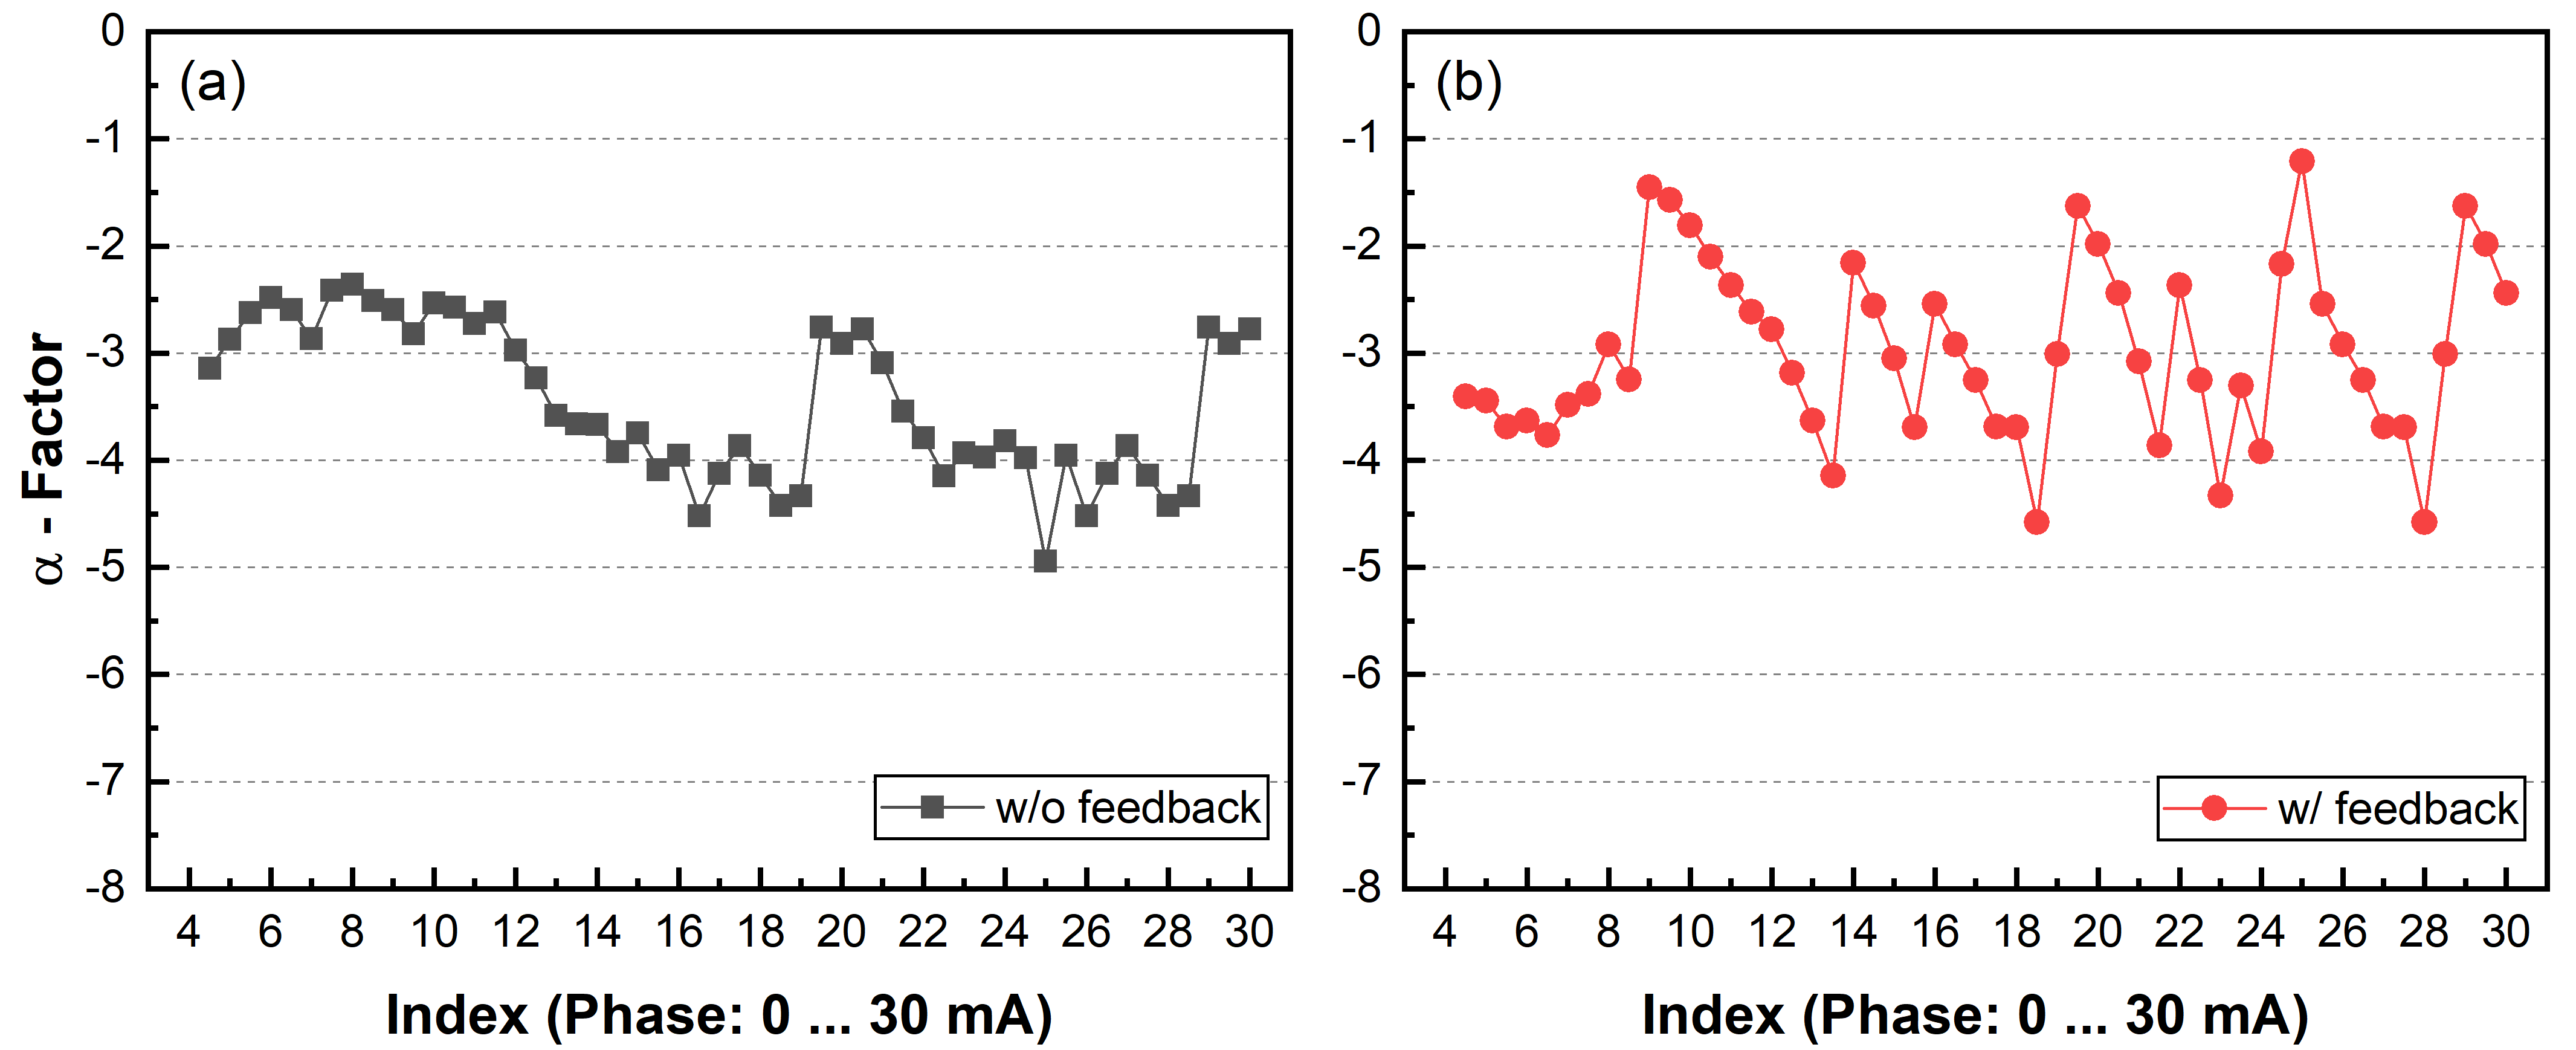
\includegraphics[width=\linewidth]{figures/Alpha_Cleaved_and_Lensed.png}
    \caption{(a) Measurement with cleaved fiber with oil, (b) measurement with lensed fiber, lower $\alpha$ parameter value is achieved.}
    \label{fig:Alpha_Cleaved_and_Lensed}
\end{figure}

% \section{Phase Noise Measurement}

